%==============================================================================
%  EILOR --- PROYECTO TECNOLÓGICO EN SISTEMAS DE INFORMACIÓN Y CIBERSEGURIDAD
%  Documento tipo tesis (integra las 4 entregas de la macro actividad)
%
%  COMPILACIÓN (Overleaf o TeX Live completo):
%     pdflatex main
%     biber   main
%     pdflatex main
%     pdflatex main
%  (En Overleaf: seleccionar compilador pdfLaTeX; el biber corre solo.)
%==============================================================================
\documentclass[12pt,a4paper,oneside]{book}

%--- Idioma y codificación --------------------------------------------------
\usepackage[utf8]{inputenc}
\usepackage[T1]{fontenc}
\usepackage[spanish,es-noshorthands,es-tabla]{babel}
\usepackage{lmodern}
\usepackage{microtype}

%--- Geometría y espaciado --------------------------------------------------
\usepackage{geometry}
\geometry{a4paper,left=3cm,right=2.5cm,top=2.5cm,bottom=2.5cm}
\usepackage{setspace}
\onehalfspacing
\usepackage{parskip}

%--- Gráficos, color, tablas ------------------------------------------------
\usepackage{graphicx}
\usepackage{xcolor}
\usepackage{float}
\usepackage{booktabs}
\usepackage{tabularx}
\usepackage{longtable}
\usepackage{array}
\usepackage{multirow}
\usepackage{ragged2e}
\usepackage{enumitem}
\usepackage{amsmath,amssymb}

%--- Diagramas --------------------------------------------------------------
\usepackage{tikz}
\usetikzlibrary{shapes.geometric,shapes.misc,arrows.meta,positioning,calc,fit,backgrounds,decorations.pathreplacing}
\usepackage{pgfplots}
\pgfplotsset{compat=1.18}

%--- Encabezados y pies -----------------------------------------------------
\usepackage{fancyhdr}
\pagestyle{fancy}
\fancyhf{}
\setlength{\headheight}{15pt}
% Marca de capítulo sin el prefijo "Capítulo N." y sin forzar mayúsculas,
% para que el encabezado no se solape con el nombre del proyecto.
\renewcommand{\chaptermark}[1]{\markboth{#1}{}}
\fancyhead[L]{\small\textsc{Proyecto EILOR}}
\fancyhead[R]{\small\itshape\nouppercase{\leftmark}}
\fancyfoot[C]{\thepage}
\renewcommand{\headrulewidth}{0.4pt}

%--- Colores corporativos del proyecto --------------------------------------
\definecolor{eilorcyan}{RGB}{0,150,180}
\definecolor{eiloremerald}{RGB}{0,160,110}
\definecolor{eilordark}{RGB}{10,20,36}
\definecolor{codebg}{RGB}{248,249,250}
\definecolor{codecomment}{RGB}{106,115,125}
\definecolor{codestring}{RGB}{3,71,120}
\definecolor{codekw}{RGB}{170,13,145}
\definecolor{codendk}{RGB}{20,110,120}
% Paleta institucional de la carátula Faceta (compartida con el manual).
\definecolor{facetred}{HTML}{A4063E}
\definecolor{facetgreen}{HTML}{93C842}
\definecolor{facetnavy}{HTML}{282660}
\definecolor{facetdark}{HTML}{161718}

%--- Listados de código -----------------------------------------------------
\usepackage{listings}
\lstdefinelanguage{JavaScript}{
  keywords={const,let,var,function,return,if,else,for,while,do,new,require,module,exports,async,await,try,catch,finally,typeof,class,this,break,switch,case,default,true,false,null,undefined,in,of,throw,delete},
  keywordstyle=\color{codekw}\bfseries,
  ndkeywords={console,JSON,Date,Math,Array,Map,Set,Object,Promise,express,app,res,req,ws,wss,process,setInterval,setTimeout,localStorage,fetch,document},
  ndkeywordstyle=\color{codendk},
  sensitive=true,
  comment=[l]{//},
  morecomment=[s]{/*}{*/},
  morestring=[b]",
  morestring=[b]',
  morestring=[b]`
}
\lstset{
  backgroundcolor=\color{codebg},
  basicstyle=\ttfamily\footnotesize,
  commentstyle=\color{codecomment}\itshape,
  stringstyle=\color{codestring},
  keywordstyle=\color{codekw}\bfseries,
  numbers=left,numberstyle=\tiny\color{gray},numbersep=8pt,
  breaklines=true,breakatwhitespace=false,
  frame=single,rulecolor=\color{gray!45},
  showstringspaces=false,
  tabsize=2,
  captionpos=b,
  extendedchars=true,
  literate=%
    {á}{{\'a}}1 {é}{{\'e}}1 {í}{{\'i}}1 {ó}{{\'o}}1 {ú}{{\'u}}1
    {Á}{{\'A}}1 {É}{{\'E}}1 {Í}{{\'I}}1 {Ó}{{\'O}}1 {Ú}{{\'U}}1
    {ñ}{{\~n}}1 {Ñ}{{\~N}}1 {ü}{{\"u}}1 {Ü}{{\"U}}1
    {¿}{{?`}}1 {¡}{{!`}}1 {°}{{\textdegree}}1 {º}{{\textordmasculine}}1
}
\lstdefinestyle{js}{language=JavaScript}
\lstdefinestyle{cpp}{language=C++}
\lstdefinestyle{bash}{language=bash,keywordstyle=\color{eiloremerald}\bfseries}
\lstdefinestyle{json}{basicstyle=\ttfamily\footnotesize}

%--- Enlaces (cargar antes de biblatex) -------------------------------------
\usepackage{csquotes}
\usepackage[hidelinks]{hyperref}
\hypersetup{
  colorlinks=true,
  linkcolor=eilordark,
  citecolor=eilorcyan,
  urlcolor=eilorcyan,
  pdftitle={EILOR --- Analizador de Espectro 2.4 GHz y Portal de Registro},
  pdfauthor={Estudiante}
}

%--- Bibliografía APA 7 -----------------------------------------------------
\usepackage[style=apa,backend=biber,sortcites=true]{biblatex}
\addbibresource{refs.bib}

%--- Comandos de ayuda ------------------------------------------------------
% Inserta una captura de pantalla real (archivo en figuras/), con marco fino.
% Uso: \captura[ancho]{ruta-sin-extension}{pie de figura}
\newcommand{\captura}[3][0.85]{%
  \begin{figure}[H]\centering
  \setlength{\fboxsep}{0pt}\setlength{\fboxrule}{0.4pt}%
  \fcolorbox{gray!45}{white}{\includegraphics[width=#1\linewidth]{figuras/#2}}%
  \caption{#3}
  \end{figure}}

% Placeholder para capturas aún no disponibles (fotografías físicas).
\newcommand{\capturapend}[2][0.7]{%
  \begin{figure}[H]\centering
  \fbox{\begin{minipage}[c][3.6cm][c]{#1\linewidth}\centering
  \textcolor{gray}{\ttfamily [ FOTOGRAFÍA PENDIENTE ]}\\[4pt]
  \small\textcolor{gray}{#2}
  \end{minipage}}
  \caption{#2}
  \end{figure}}

\newcommand{\code}[1]{\texttt{\small #1}}

% Datos de despliegue de referencia (editar si cambian)
\newcommand{\plataformaurl}{\url{https://esp.orellanadigitalco.trade/}}
\newcommand{\repourl}{\url{https://github.com/ptandazoz9827/evil-esp32}}

\begin{document}

%============================ PORTADA =======================================
%============================ PORTADA =======================================
% Carátula institucional con el mismo diseño Faceta utilizado en el manual.
\begin{titlepage}
\thispagestyle{empty}
\begin{tikzpicture}[remember picture,overlay]
  \coordinate (NW) at (current page.north west);
  \node[anchor=north west,inner sep=0] at (NW)
    {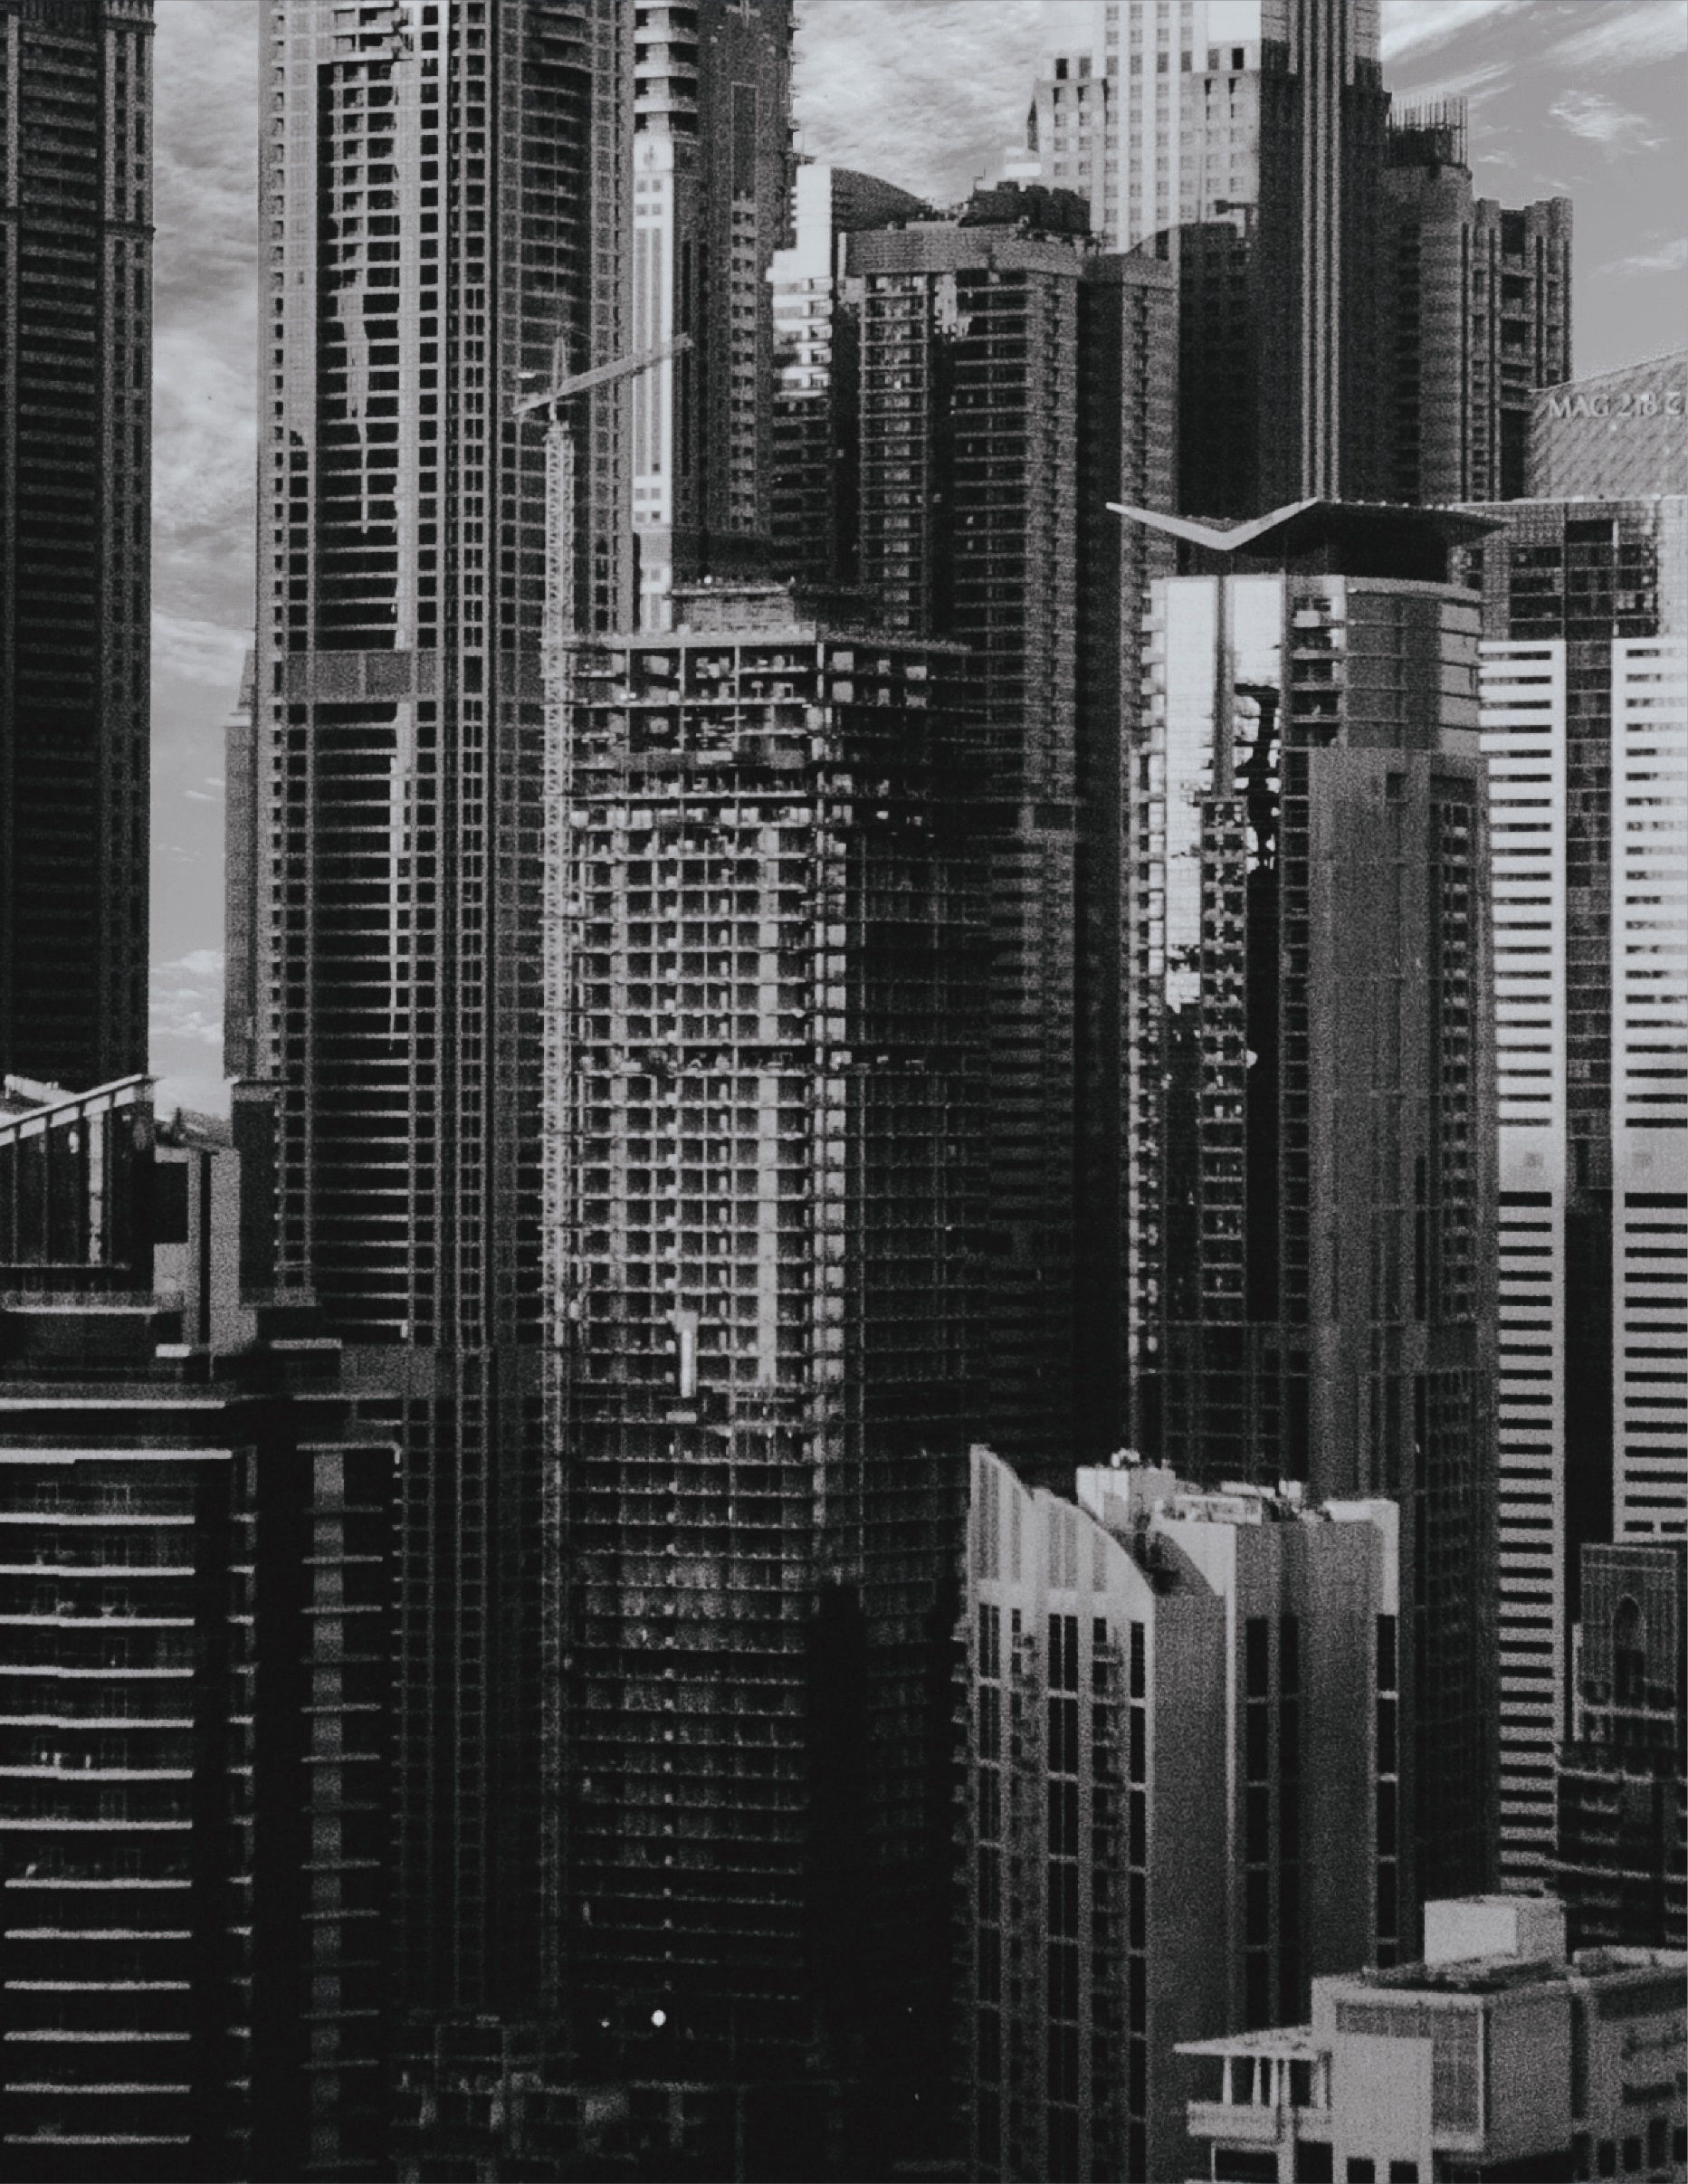
\includegraphics[width=\paperwidth,height=\paperheight]{figuras/portada-ciudad}};
  \fill[facetgreen] ([yshift=-18mm]NW) rectangle ([xshift=9mm,yshift=-95mm]NW);
  \node[anchor=north west,text=white,align=left,font=\sffamily\bfseries\large]
    at ([xshift=16mm,yshift=-24mm]NW) {PROYECTO TECNOLÓGICO};
  \node[anchor=north west,text=white,align=left,font=\sffamily\small]
    at ([xshift=16mm,yshift=-33mm]NW)
    {Desarrollo en Sistemas de Información y Ciberseguridad};
  \fill[facetred,opacity=0.95]
    ([yshift=-142mm]NW) rectangle ([xshift=\paperwidth,yshift=-214mm]NW);
  \node[anchor=west,text=white,align=left,text width=175mm,font=\sffamily]
    at ([xshift=17mm,yshift=-177mm]NW)
    {{\fontsize{15}{17}\selectfont EILOR}\\[4pt]
     {\fontsize{29}{33}\selectfont\bfseries Analizador táctico de espectro}\\[-1pt]
     {\fontsize{29}{33}\selectfont\bfseries 2.4\,GHz, radar BLE y portal de registro}\\[6pt]
     {\fontsize{11}{13}\selectfont\itshape Sistema basado en ESP32, Node.js y WebSocket en tiempo real}};
  \fill[facetnavy] ([yshift=-214mm]NW) rectangle ([xshift=\paperwidth,yshift=-241mm]NW);
  \node[anchor=west,text=white,align=left,text width=175mm,font=\sffamily\bfseries]
    at ([xshift=17mm,yshift=-227.5mm]NW)
    {DESARROLLO DE PROYECTO TECNOLÓGICO EN SISTEMAS DE INFORMACIÓN Y CIBERSEGURIDAD};
  \fill[white,opacity=0.92] ([yshift=-241mm]NW) rectangle ([xshift=\paperwidth,yshift=-297mm]NW);
  \node[anchor=north west,text=facetdark,align=left,font=\sffamily,text width=120mm]
    at ([xshift=17mm,yshift=-247mm]NW)
    {\textbf{\color{facetred}Autor}\\[2pt]
     Pablo Alejandro Tandazo Zarango\\
     \textbf{Tutor / docente}\\[2pt]
     Ing. Marco Silva, Mg};
  \node[anchor=south east,inner sep=0] at ([xshift=\paperwidth-16mm,yshift=-289mm]NW)
    {
\includegraphics[width=52mm]{figuras/logo-sic}};
  \node[anchor=south west,text=facetnavy,font=\sffamily\small\bfseries]
    at ([xshift=17mm,yshift=-286mm]NW) {Ciudad, provincia};
  \node[anchor=south west,text=facetnavy,font=\sffamily\small\bfseries]
    at ([xshift=17mm,yshift=-292mm]NW) {\today};
\end{tikzpicture}
\end{titlepage}


%============================ FRONTAL =======================================
\frontmatter\pagenumbering{roman}\setcounter{page}{2}
%============================ RESUMEN =======================================
\chapter*{Resumen ejecutivo}
\addcontentsline{toc}{chapter}{Resumen ejecutivo}
\markboth{RESUMEN EJECUTIVO}{}

El presente proyecto documenta el diseño, la implementación y la validación de \textbf{EILOR}, un sistema integral de \emph{monitoreo del espectro radioeléctrico de 2.4~GHz} y \emph{gestión de acceso de invitados} orientado a pequeños negocios y a laboratorios de aprendizaje en ciberseguridad. El sistema combina un dispositivo de hardware de bajo costo basado en el microcontrolador \textbf{ESP32}, que integra ambas radios y escanea redes Wi\nobreakdash-Fi (canales 1 al 13) y balizas Bluetooth de Baja Energía (BLE) en modos dedicados conmutables, con un \textbf{servidor de tiempo real} construido sobre Node.js, Express y WebSocket que agrega, analiza, persiste y visualiza los datos capturados en un tablero de mando (\emph{dashboard}) web.

EILOR incorpora cuatro modos operativos ---análisis de espectro Wi\nobreakdash-Fi, radar de proximidad BLE por RSSI, punto de acceso (SoftAP) con \emph{portal cautivo} de registro de invitados y modo de telemetría/reposo--- gobernados de forma remota mediante comandos WebSocket. En la capa de análisis, el servidor calcula un \emph{puntaje de interferencia} por canal que pondera el solapamiento de canales adyacentes y la intensidad de señal, recomienda el canal más limpio del conjunto no solapado 1/6/11 y detecta puntos de acceso sospechosos de tipo \emph{gemelo malicioso} (\emph{evil twin}). Adicionalmente, se implementó una capa de seguridad con autenticación por token de sesión para las acciones de control, un token opcional de dispositivo para restringir la ingesta de datos y un mecanismo de identificación de fabricante mediante prefijos OUI, junto con la detección de direcciones MAC aleatorizadas por privacidad.

La validación funcional confirmó la operación de extremo a extremo del sistema: ingesta de escaneos, análisis de canales, persistencia con recuperación tras reinicio, control de acceso (respuestas 401/200 según credenciales) y registro de invitados desde el portal cautivo con \emph{buffer} de reenvío ante caídas de enlace. El documento presenta, además, el análisis de desempeño, la estimación de costos con curva~S, la evaluación de impacto ambiental, la propuesta de escalabilidad y los manuales de usuario y técnico, cumpliendo la totalidad de los entregables definidos en la macro actividad.

\vspace{0.6cm}
\noindent\textbf{Palabras clave:} espectro 2.4~GHz, ESP32, IEEE 802.11, Bluetooth Low Energy, WebSocket, portal cautivo, ciberseguridad, gemelo malicioso, OUI, tiempo real.

\vspace{0.4cm}
\hrule
\vspace{0.4cm}

\noindent\textbf{\emph{Abstract.}} This project documents the design, implementation and validation of \textbf{EILOR}, an integrated system for \emph{2.4~GHz radio-frequency spectrum monitoring} and \emph{guest-access management} aimed at small businesses and cybersecurity learning labs. It couples a low-cost \textbf{ESP32}-based device ---which integrates both radios and scans Wi-Fi networks (channels 1--13) and Bluetooth Low Energy (BLE) beacons in dedicated switchable modes--- with a \textbf{real-time server} built on Node.js, Express and WebSocket that aggregates, analyses, persists and visualises the captured data on a web dashboard. EILOR provides four operating modes, an adjacency-aware channel-interference score, evil-twin access-point detection, OUI-based vendor identification, randomized-MAC awareness, and a token-based security layer. End-to-end validation confirmed data ingestion, channel analysis, restart-safe persistence, access control and captive-portal guest registration with offline buffering.

\tableofcontents
\listoffigures
\listoftables
\cleardoublepage

%============================ CUERPO ========================================
\mainmatter\pagenumbering{arabic}\setcounter{page}{1}

%============================ INTRODUCCIÓN ==================================
\chapter{Introducción}
\label{cap:introduccion}

La banda de 2.4~GHz constituye hoy uno de los recursos radioeléctricos más congestionados del entorno cotidiano. En ella coexisten redes Wi\nobreakdash-Fi bajo el estándar IEEE~802.11, dispositivos Bluetooth y Bluetooth de Baja Energía (BLE), teléfonos inalámbricos, hornos de microondas y una densidad creciente de dispositivos del Internet de las Cosas (IoT). Esta coexistencia, sumada a que solo tres de los trece canales de 2.4~GHz (1, 6 y 11) no se solapan entre sí, provoca degradaciones de rendimiento difíciles de diagnosticar sin instrumentación especializada \parencite{gast2005,bianchi2000}. Los analizadores de espectro comerciales, si bien precisos, resultan costosos y poco accesibles para pequeños negocios, instituciones educativas y laboratorios de aprendizaje.

Paralelamente, la seguridad de las redes inalámbricas se ha vuelto una preocupación central. Ataques como el punto de acceso \emph{gemelo malicioso} (\emph{evil twin}), en el que un atacante replica el nombre de una red legítima para interceptar tráfico, explotan precisamente la naturaleza abierta del medio y la confianza del usuario \parencite{callegati2009,owasp2021}. Detectar la presencia de estos puntos de acceso y comprender la ocupación del espectro son capacidades formativas esenciales para quien se inicia en la ciberseguridad.

El proyecto \textbf{EILOR} nace en la intersección de ambas necesidades: ofrecer una plataforma \emph{asequible, didáctica y funcional} que permita, por un lado, \emph{visualizar y analizar} el espectro de 2.4~GHz en tiempo real y, por otro, ejercer un \emph{control de acceso} responsable mediante un punto de acceso propio con portal cautivo de registro de invitados ---al estilo del Wi\nobreakdash-Fi de una cafetería---. Todo ello se construye sobre hardware de bajo costo (ESP32) y una pila de software abierta (Node.js, Express, WebSocket).

\section{Justificación}
La elección del microcontrolador ESP32 responde a que integra, en un mismo encapsulado y por un costo reducido, radios Wi\nobreakdash-Fi y Bluetooth/BLE, capacidad de procesamiento suficiente para escaneo activo y una pila TCP/IP completa \parencite{espressif2023}. Frente a soluciones cerradas, EILOR privilegia la \emph{transparencia} (código propio y modular), la \emph{reproducibilidad} (persistencia en archivos JSON sin dependencias nativas) y el \emph{valor pedagógico}: cada componente ---desde el cálculo de interferencia por canal hasta la autenticación por token--- es observable y auditable.

\section{Alcance y delimitación}
El sistema se circunscribe a la banda de 2.4~GHz y a los canales de \emph{advertising} de BLE (37, 38 y 39). No abarca la banda de 5~GHz ni la decodificación de tramas de datos de terceros; el escaneo Wi\nobreakdash-Fi se limita a la información de baliza (SSID, BSSID, canal, RSSI y tipo de cifrado) que la propia API del ESP32 expone. La funcionalidad de punto de acceso y portal cautivo está concebida para operar sobre una \emph{red propia}, con un nombre de red identificable y un aviso explícito de registro, en cumplimiento de principios éticos y de protección de datos; su uso para suplantar redes ajenas queda expresamente fuera del alcance autorizado del proyecto.

\section{Estructura del documento}
El documento integra los cuatro entregables de la macro actividad. El Capítulo~\ref{cap:problema} delimita el problema en sus niveles macro, meso y micro; el Capítulo~\ref{cap:marco} desarrolla el marco teórico; el Capítulo~\ref{cap:objetivos} formula los objetivos bajo criterios SMART; y el Capítulo~\ref{cap:arquitectura} presenta la arquitectura y las tecnologías (Entrega~1). El Capítulo~\ref{cap:diseno} detalla el diseño; el Capítulo~\ref{cap:implementacion} documenta la implementación con el código real del sistema; y el Capítulo~\ref{cap:pruebas} expone el plan y los resultados de pruebas de seguridad (Entrega~2). Los Capítulos~\ref{cap:desempeno} a \ref{cap:manuales} abordan el desempeño, el análisis económico\nobreakdash-ambiental con curva~S, la escalabilidad y los manuales (Entrega~3). Finalmente, el Capítulo~\ref{cap:conclusiones} presenta las conclusiones y la sustentación (Entrega~4), seguido de las referencias y los anexos.


% ---- ENTREGA 1: FUNDAMENTACIÓN Y PLANIFICACIÓN ----
%============================ PROBLEMA (ENTREGA 1) ==========================
\chapter{Planteamiento y delimitación del problema}
\label{cap:problema}

\section{Descripción del problema}
La saturación de la banda no licenciada de 2.4~GHz produce, en entornos reales, síntomas recurrentes: caídas de rendimiento, latencias variables, desconexiones intermitentes y una experiencia de usuario deficiente. La causa suele ser invisible para el usuario final ---interferencia co\nobreakdash-canal y de canal adyacente, exceso de puntos de acceso compitiendo por el mismo canal, o dispositivos BLE saturando las frecuencias de \emph{advertising}--- y su diagnóstico exige instrumentación que la mayoría de pequeños negocios no posee. A esta problemática técnica se suma una dimensión de seguridad: la facilidad con que puede desplegarse un punto de acceso que imite a una red legítima hace que los usuarios sean vulnerables a la captura de información si no existen mecanismos de concientización y control \parencite{owasp2021,callegati2009}.

El problema que aborda EILOR se formula así: \emph{no existe, para el pequeño negocio o el laboratorio educativo, una herramienta asequible que permita simultáneamente (i)~diagnosticar la ocupación e interferencia del espectro de 2.4~GHz en tiempo real, (ii)~identificar dispositivos y posibles amenazas inalámbricas, y (iii)~gestionar de forma responsable el acceso de invitados a una red propia}.

\section{Contextualización}

\subsection{Nivel macro}
A escala global, la proliferación de dispositivos IoT ---proyectada en decenas de miles de millones de unidades--- presiona de manera sostenida las bandas no licenciadas \parencite{akyildiz2006}. La gestión eficiente del espectro se ha convertido en una línea de investigación consolidada, desde la radio cognitiva hasta las técnicas de \emph{spectrum sensing} \parencite{yucek2009}. En este contexto macro, disponer de instrumentos de medición democratizados es un facilitador tanto del rendimiento de las redes como de la formación de profesionales.

\subsection{Nivel meso}
En el ámbito de las pequeñas y medianas organizaciones (cafeterías, comercios, oficinas, instituciones educativas), la conectividad Wi\nobreakdash-Fi es un servicio esperado, pero rara vez se administra con criterio técnico. La selección del canal se deja habitualmente al valor por defecto del router, y la red de invitados ---cuando existe--- no distingue entre usuarios ni recopila información de contacto útil para el negocio. La ausencia de visibilidad sobre el espectro y sobre los dispositivos presentes limita tanto la optimización del servicio como la respuesta ante incidentes.

\subsection{Nivel micro}
En el nivel micro ---el de un local concreto o un laboratorio de aula--- el problema se materializa en decisiones cotidianas: ¿en qué canal debería operar el punto de acceso para minimizar interferencia?, ¿cuántos y qué tipo de dispositivos hay alrededor?, ¿existe algún punto de acceso que suplante el nombre de la red del negocio?, ¿cómo registrar de forma sencilla a los invitados que se conectan? EILOR responde a estas preguntas concretas con una interfaz única y datos en vivo.

\section{Formulación del problema}
\textbf{Pregunta general:} ¿Cómo diseñar e implementar un sistema de bajo costo que permita el monitoreo en tiempo real del espectro de 2.4~GHz, la identificación de dispositivos y amenazas inalámbricas, y la gestión responsable del acceso de invitados mediante un portal cautivo?

\noindent\textbf{Preguntas específicas:}
\begin{itemize}[leftmargin=1.4em]
  \item ¿Qué arquitectura de hardware y software satisface el escaneo de Wi\nobreakdash-Fi y BLE (en modos dedicados conmutables) con visualización en tiempo real?
  \item ¿Qué algoritmo de análisis permite estimar la interferencia por canal y recomendar el canal óptimo?
  \item ¿Cómo detectar puntos de acceso de tipo gemelo malicioso e identificar el fabricante de un dispositivo a partir de su dirección MAC?
  \item ¿Qué mecanismos de seguridad y de protección de datos deben incorporarse para un portal de registro de invitados?
\end{itemize}

\section{Objetivos preliminares y viabilidad}
El problema es abordable con recursos accesibles: un ESP32 (costo aproximado inferior a USD~10), una pantalla OLED, un pulsador y un servidor Node.js ejecutable en cualquier equipo o en la nube. La viabilidad técnica se sustenta en la capacidad dual\nobreakdash-radio del ESP32 \parencite{espressif2023} y en la madurez de las tecnologías web de tiempo real \parencite{rfc6455}. Los objetivos formales se detallan en el Capítulo~\ref{cap:objetivos}.

%============================ MARCO TEÓRICO (ENTREGA 1) =====================
\chapter{Marco teórico y antecedentes}
\label{cap:marco}

Este capítulo sintetiza los fundamentos conceptuales y los antecedentes que sustentan el proyecto, organizados en cinco ejes: el medio radioeléctrico de 2.4~GHz, las tecnologías Wi\nobreakdash-Fi y BLE, los modelos de análisis de espectro y de localización por RSSI, la seguridad inalámbrica y las tecnologías de software de tiempo real.

\section{El espectro de 2.4 GHz y la interferencia de canal}
La banda ISM de 2.4~GHz se divide, en la mayoría de las regiones, en trece canales Wi\nobreakdash-Fi separados 5~MHz entre sí. Dado que cada canal ocupa aproximadamente 20--22~MHz, canales contiguos se solapan y solo el conjunto \{1, 6, 11\} resulta mutuamente no solapado \parencite{gast2005}. La interferencia se clasifica en \emph{co\nobreakdash-canal} (dos emisores en el mismo canal, que comparten el medio mediante CSMA/CA) y de \emph{canal adyacente} (emisores en canales cercanos cuyo espectro se traslapa, degradando la relación señal\nobreakdash-ruido). El modelo analítico de Bianchi \parencite{bianchi2000} sobre la función de coordinación distribuida (DCF) de IEEE~802.11 explica por qué el rendimiento agregado decae al aumentar el número de estaciones que contienden por un canal, justificando la importancia de seleccionar canales poco congestionados.

\section{Wi-Fi (IEEE 802.11) y escaneo pasivo/activo}
El estándar IEEE~802.11 \parencite{ieee80211} define los mecanismos de descubrimiento de redes: en el escaneo \emph{pasivo}, la estación escucha las tramas \emph{beacon} que los puntos de acceso emiten periódicamente; en el \emph{activo}, envía \emph{probe requests} y espera \emph{probe responses}. De estas tramas se extraen el identificador de red (SSID), la dirección física del punto de acceso (BSSID), el canal, la intensidad de señal recibida (RSSI) y el tipo de cifrado. EILOR utiliza el escaneo que ofrece la API del ESP32 para obtener estos campos sin decodificar tráfico de datos de terceros, respetando así la delimitación ética del proyecto.

\section{Bluetooth Low Energy (BLE)}
BLE, definido a partir de la especificación Bluetooth Core \parencite{bluetooth54} y descrito en profundidad por Heydon \parencite{heydon2013}, emplea 40 canales de 2~MHz, de los cuales tres ---los canales 37, 38 y 39, ubicados en 2402, 2426 y 2480~MHz--- se reservan para \emph{advertising} (anuncio de presencia). Un dispositivo BLE emite paquetes de \emph{advertising} que otros pueden detectar sin establecer conexión, exponiendo un nombre, una dirección y una potencia de señal. EILOR aprovecha estos paquetes para su "radar de proximidad", estimando la cercanía relativa de las balizas a partir del RSSI.

\section{Estimación de distancia por RSSI}
La conversión de RSSI a distancia se apoya en el modelo de pérdida de trayectoria logarítmica \parencite{rappaport2002}, según el cual la potencia recibida decae proporcionalmente al logaritmo de la distancia:
\begin{equation}
RSSI(d) = RSSI(d_0) - 10\,n \log_{10}\!\left(\frac{d}{d_0}\right),
\label{eq:pathloss}
\end{equation}
donde $n$ es el exponente de pérdida de trayectoria (típicamente entre 2 en espacio libre y 4 en interiores con obstáculos) y $d_0$ una distancia de referencia. Despejando $d$ se obtiene una estimación de distancia que, aunque sensible al entorno, resulta suficiente para un posicionamiento radial cualitativo, tal como demostró el sistema RADAR de Bahl y Padmanabhan \parencite{bahl2000}, pionero en la localización en interiores basada en RSSI.

\section{Identificación de fabricante por OUI y MAC aleatorizadas}
Los primeros tres octetos de una dirección MAC constituyen el \emph{Organizationally Unique Identifier} (OUI), asignado por la IEEE a cada fabricante \parencite{ieeeoui}. Consultando el OUI puede inferirse el fabricante de un dispositivo. No obstante, desde hace varios años los sistemas operativos móviles emplean \emph{aleatorización de MAC} para preservar la privacidad, generando direcciones localmente administradas ---identificables porque el segundo bit menos significativo del primer octeto está a 1--- que impiden el rastreo persistente \parencite{martin2017}. EILOR implementa tanto la búsqueda de fabricante por OUI como la detección de direcciones aleatorizadas, informando al analista cuándo un dispositivo oculta su identidad real.

\section{Seguridad inalámbrica: gemelo malicioso y buenas prácticas}
El ataque de \emph{gemelo malicioso} consiste en desplegar un punto de acceso que anuncia el mismo SSID que una red legítima para inducir a las víctimas a conectarse a él, habilitando ataques de intermediario (\emph{man\nobreakdash-in\nobreakdash-the\nobreakdash-middle}) \parencite{callegati2009}. Una heurística de detección consiste en identificar un mismo SSID anunciado por múltiples BSSID distintos, señal de posible suplantación. Los controles recomendados por marcos como OWASP \parencite{owasp2021} ---autenticación robusta, minimización de datos y transparencia hacia el usuario--- guían el diseño de la capa de seguridad y del portal de registro de EILOR.

\section{Tecnologías de software de tiempo real}
La comunicación bidireccional de baja latencia entre el hardware, el servidor y los clientes web se sustenta en el protocolo WebSocket \parencite{rfc6455}, que mantiene una conexión persistente sobre TCP evitando el costo de las peticiones HTTP repetidas. El servidor se organiza siguiendo el estilo arquitectónico REST \parencite{fielding2002} para sus endpoints de consulta y control, y se ejecuta sobre Node.js \parencite{nodejs2024}, cuyo modelo de E/S no bloqueante resulta idóneo para manejar numerosas conexiones concurrentes. El portal cautivo, por su parte, se apoya en la manipulación de las consultas DNS \parencite{rfc1035} para redirigir a los clientes a la página de registro. Los fundamentos generales de redes que enmarcan estas tecnologías se encuentran en obras de referencia como las de Tanenbaum y Wetherall \parencite{tanenbaum2011} y Kurose y Ross \parencite{kurose2017}.

\section{Síntesis de antecedentes}
La Tabla~\ref{tab:antecedentes} resume cómo los antecedentes revisados aportan a cada componente de EILOR.

\begin{table}[H]
\centering
\caption{Aporte de los antecedentes a los componentes de EILOR}
\label{tab:antecedentes}
\footnotesize
\begin{tabularx}{\linewidth}{@{}>{\raggedright\arraybackslash}p{3.1cm} >{\raggedright\arraybackslash}X >{\raggedright\arraybackslash}p{4.0cm}@{}}
\toprule
\textbf{Componente} & \textbf{Fundamento / antecedente} & \textbf{Referencia} \\
\midrule
Análisis de canal & Interferencia y DCF en 802.11 & \textcite{gast2005}; \textcite{bianchi2000} \\
Escaneo Wi-Fi & Tramas \emph{beacon}/\emph{probe} & \textcite{ieee80211} \\
Radar BLE & Canales de \emph{advertising} & \textcite{bluetooth54}; \textcite{heydon2013} \\
Distancia por RSSI & Modelo de pérdida de trayectoria & \textcite{rappaport2002}; \textcite{bahl2000} \\
Fabricante / MAC & OUI y aleatorización & \textcite{ieeeoui}; \textcite{martin2017} \\
Detección \emph{evil twin} & MITM y buenas prácticas & \textcite{callegati2009}; \textcite{owasp2021} \\
Comunicación en vivo & WebSocket y REST & \textcite{rfc6455}; \textcite{fielding2002} \\
Portal cautivo & Redirección DNS & \textcite{rfc1035} \\
Plataforma de servidor & Node.js, E/S no bloqueante & \textcite{nodejs2024} \\
\bottomrule
\end{tabularx}
\end{table}

%============================ OBJETIVOS (ENTREGA 1) =========================
\chapter{Objetivos}
\label{cap:objetivos}

\section{Objetivo general}
Diseñar, implementar y validar un sistema de bajo costo, denominado EILOR, para el monitoreo en tiempo real del espectro de 2.4~GHz, la identificación de dispositivos y amenazas inalámbricas, y la gestión responsable del acceso de invitados mediante un punto de acceso con portal cautivo de registro, integrando hardware ESP32 y un servidor web de tiempo real.

\section{Objetivos específicos}
\begin{enumerate}[label=\textbf{OE\arabic*.},leftmargin=2.4em]
  \item Desarrollar un firmware para ESP32 que escanee redes Wi\nobreakdash-Fi (canales 1--13) y balizas BLE (canales 37--39) en modos dedicados conmutables y transmita los resultados en tiempo real mediante WebSocket.
  \item Construir un servidor modular en Node.js que agregue los datos, calcule un puntaje de interferencia por canal, recomiende el canal óptimo y detecte puntos de acceso de tipo gemelo malicioso.
  \item Implementar la identificación de fabricante por OUI y la detección de direcciones MAC aleatorizadas para enriquecer el inventario de dispositivos.
  \item Incorporar una capa de seguridad con autenticación por token de sesión para el control y un token opcional de dispositivo para la ingesta de datos.
  \item Desarrollar un punto de acceso (SoftAP) con portal cautivo que registre invitados (nombre, apellido y teléfono) y persista la información en el servidor, con reenvío ante caídas de enlace.
  \item Validar funcionalmente el sistema completo mediante pruebas de ingesta, análisis, persistencia, control de acceso y registro de invitados.
\end{enumerate}

\section{Matriz de objetivos bajo criterios SMART}
Cada objetivo específico se formuló siguiendo los criterios SMART (específico, medible, alcanzable, relevante y temporal). La Tabla~\ref{tab:smart} presenta la matriz de verificación.

\begin{table}[H]
\centering
\caption{Matriz SMART de los objetivos específicos}
\label{tab:smart}
\footnotesize
\begin{tabularx}{\linewidth}{@{}c X X l@{}}
\toprule
\textbf{OE} & \textbf{Indicador medible} & \textbf{Criterio de logro (alcanzable/relevante)} & \textbf{Plazo} \\
\midrule
OE1 & N.º de canales escaneados y latencia de ciclo & 13 canales Wi-Fi + 3 BLE; ciclo $\le$ 3~s & Sem. 6 \\
OE2 & Puntaje por canal y canal recomendado & Cálculo para 13 canales y salida 1/6/11 & Sem. 7 \\
OE3 & Cobertura del catálogo OUI & $\ge$ 120 prefijos; detección de MAC aleatoria & Sem. 7 \\
OE4 & Respuestas de control autenticado & 401 sin token / 200 con token & Sem. 7 \\
OE5 & Registros entregados por el portal & 100\,\% de envíos con enlace; \emph{buffer} sin enlace & Sem. 7 \\
OE6 & Casos de prueba superados & $\ge$ 90\,\% de casos funcionales OK & Sem. 8 \\
\bottomrule
\end{tabularx}
\end{table}

\noindent La justificación de cada objetivo se articula con las preguntas específicas del Capítulo~\ref{cap:problema}: OE1 y OE2 responden a la necesidad de diagnóstico del espectro; OE3 y OE6 a la identificación de dispositivos y su validación; OE4 y OE5 a la gestión responsable y segura del acceso de invitados.

%============================ ARQUITECTURA (ENTREGA 1) ======================
\chapter{Propuesta técnica y arquitectura}
\label{cap:arquitectura}

\section{Visión general de la arquitectura}
EILOR adopta una arquitectura de tres capas físicas ---\emph{dispositivo}, \emph{servidor} y \emph{clientes}--- comunicadas mediante WebSocket sobre TLS (WSS) a través de un túnel público, y complementadas por una API REST para consultas y control. La Figura~\ref{fig:arquitectura} sintetiza el flujo.

\begin{figure}[H]
\centering
\setlength{\fboxsep}{0pt}\setlength{\fboxrule}{0.4pt}%
\fcolorbox{gray!45}{white}{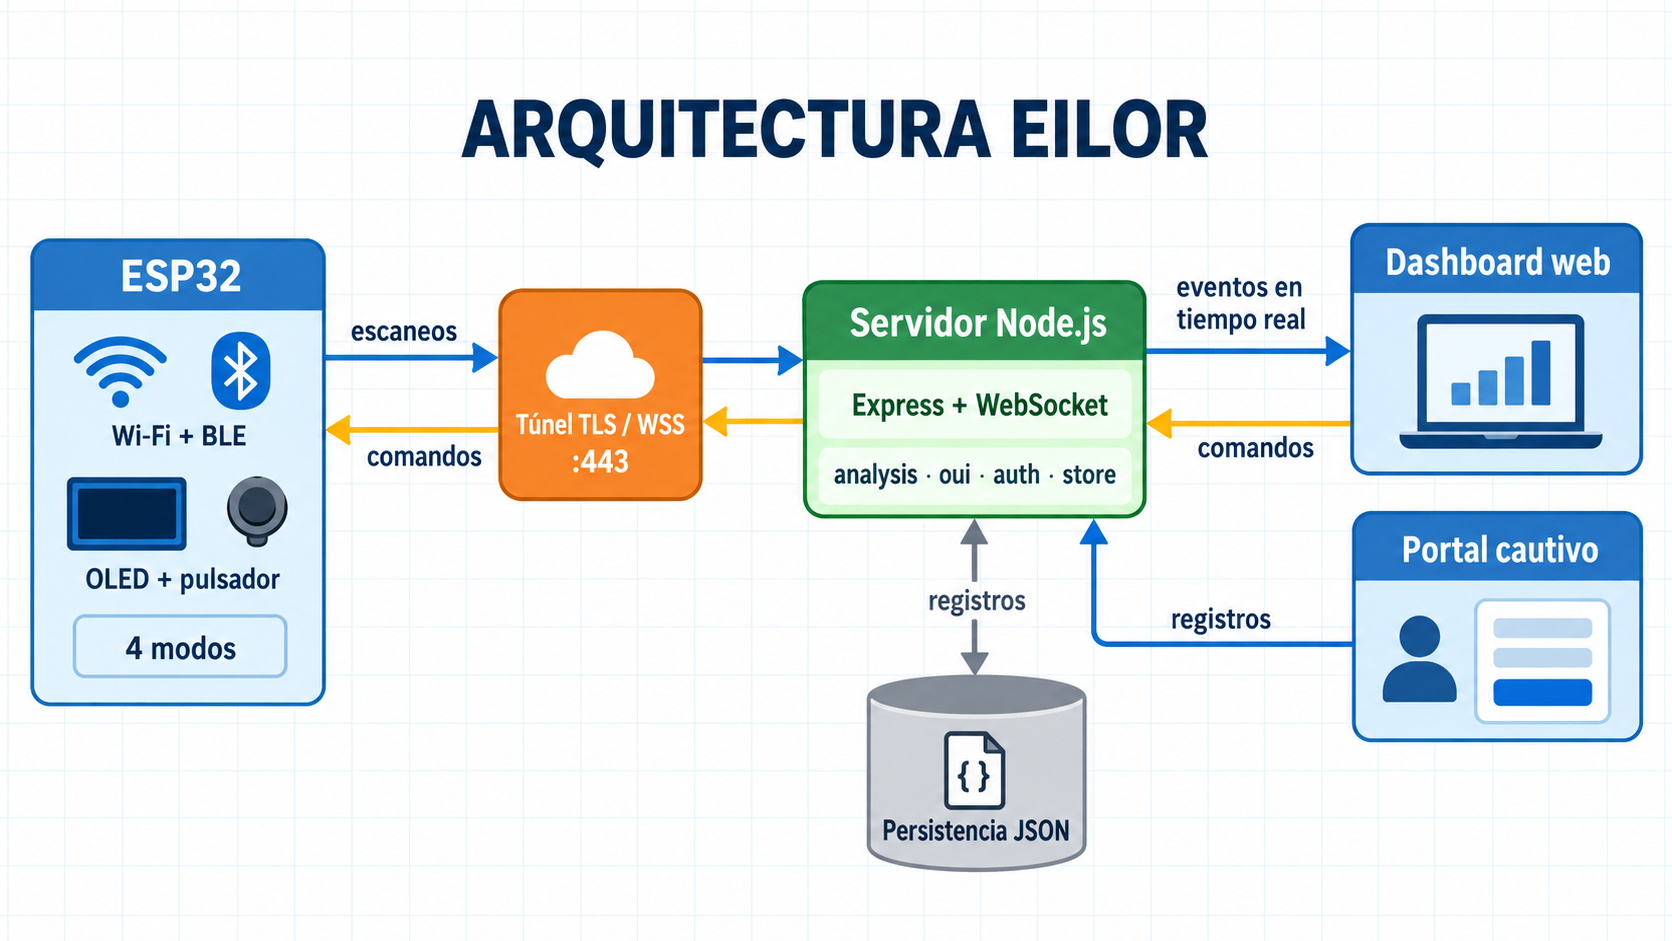
\includegraphics[width=0.98\linewidth]{figuras/arquitectura-eilor}}
\caption{Arquitectura general de EILOR: dispositivo, túnel, servidor modular, persistencia y clientes. La imagen resume el flujo; los contratos de mensajes se especifican en las tablas y diagramas de secuencia del capítulo.}
\label{fig:arquitectura}
\end{figure}

\section{Descripción de las capas}
\subsection{Capa de dispositivo (ESP32)}
El firmware implementa cuatro modos operativos conmutables por un pulsador físico o por comando remoto: (0)~análisis de espectro Wi\nobreakdash-Fi, (1)~radar de proximidad BLE, (2)~punto de acceso SoftAP con portal cautivo y (3)~telemetría/reposo. Una pantalla OLED SSD1306 muestra el estado local, y el dispositivo mantiene una conexión WebSocket persistente con el servidor para transmitir escaneos y recibir comandos.

\subsection{Capa de servidor (Node.js)}
El servidor centraliza la lógica de negocio en cuatro módulos desacoplados dentro de \code{lib/}: \code{analysis} (puntaje de interferencia y detección de gemelos maliciosos), \code{oui} (identificación de fabricante y MAC aleatorizadas), \code{store} (persistencia y series temporales) y \code{auth} (autenticación por token). Sobre ellos, \code{server.js} expone un servidor WebSocket y una API REST de catorce \emph{endpoints}.

\subsection{Capa de clientes}
Dos tipos de clientes consumen el sistema: el \emph{dashboard} web, que recibe actualizaciones en vivo por WebSocket y visualiza el espectro, el radar, la tabla de dispositivos y los registros; y los \emph{invitados}, que al conectarse al SoftAP son redirigidos por el portal cautivo a un formulario de registro.

\section{Selección de tecnologías}
La Tabla~\ref{tab:stack} justifica la pila tecnológica seleccionada.

\begin{table}[H]
\centering
\caption{Pila tecnológica y justificación}
\label{tab:stack}
\footnotesize
\begin{tabularx}{\linewidth}{@{}l l X@{}}
\toprule
\textbf{Capa} & \textbf{Tecnología} & \textbf{Justificación} \\
\midrule
Hardware & ESP32 & Radios Wi-Fi + BLE integradas, bajo costo, pila TCP/IP \parencite{espressif2023} \\
Pantalla & OLED SSD1306 & Bajo consumo, I\textsuperscript{2}C, suficiente para telemetría local \\
Firmware & C++ / Arduino & Ecosistema maduro de librerías (WebSockets, BLE, DNSServer) \\
Servidor & Node.js + Express & E/S no bloqueante idónea para tiempo real \parencite{nodejs2024} \\
Tiempo real & WebSocket (\code{ws}) & Canal bidireccional persistente de baja latencia \parencite{rfc6455} \\
Persistencia & Archivos JSON & Sin dependencias nativas; portable y auditable \\
Portal cautivo & DNSServer + WebServer & Redirección DNS y formulario embebido \parencite{rfc1035} \\
Frontend & HTML/CSS/JS & Sin framework; ligero y transparente \\
Despliegue & PM2 & Gestión de procesos, reinicio y persistencia de arranque \\
\bottomrule
\end{tabularx}
\end{table}

\section{Especificaciones técnicas iniciales}
\begin{itemize}[leftmargin=1.4em]
  \item \textbf{Banda:} 2.4~GHz; canales Wi-Fi 1--13; canales BLE de advertising 37, 38 y 39.
  \item \textbf{Frecuencia de escaneo:} ciclo de $\sim$3~s por modo activo.
  \item \textbf{Telemetría:} \emph{heartbeat} cada 3~s; \emph{watchdog} de desconexión a los 15~s.
  \item \textbf{Series temporales:} una muestra por minuto, retención de 720 muestras ($\sim$12~h).
  \item \textbf{Persistencia:} \emph{snapshot} de dispositivos cada 30~s y volcado en apagado ordenado.
  \item \textbf{Seguridad:} token de sesión (TTL 24~h) para control; token de dispositivo opcional para ingesta.
\end{itemize}


% ---- ENTREGA 2: DESARROLLO TÉCNICO ----
%============================ DISEÑO (ENTREGA 2) ============================
\chapter{Diseño detallado}
\label{cap:diseno}

\section{Diagrama de componentes}
La Figura~\ref{fig:componentes} descompone el sistema en sus componentes de software y sus dependencias. En el servidor, \code{server.js} orquesta cuatro módulos especializados; en el firmware, el bucle principal coordina el escaneo, el portal cautivo y el enlace WebSocket.

\begin{figure}[H]
\centering
\begin{tikzpicture}[
  comp/.style={rectangle,draw,thick,rounded corners=2pt,align=center,font=\small,
               minimum width=2.7cm,minimum height=0.9cm},
  grp/.style={rectangle,draw,dashed,rounded corners=4pt,inner sep=8pt},
  arr/.style={-{Latex[length=2mm]},thick},
  lbl/.style={font=\scriptsize\itshape}
]
% Servidor
\node[comp,fill=eiloremerald!12] (srv) {server.js};
\node[comp,fill=eiloremerald!6,below left=1.0cm and 0.1cm of srv] (an) {lib/analysis};
\node[comp,fill=eiloremerald!6,below=1.0cm of srv] (ou) {lib/oui};
\node[comp,fill=eiloremerald!6,below right=1.0cm and 0.1cm of srv] (au) {lib/auth};
\node[comp,fill=eiloremerald!6,below=2.4cm of srv] (st) {lib/store};
\node[comp,fill=blue!7,below=0.7cm of st] (data) {data/*.json};

\draw[arr] (srv) -- (an); \draw[arr] (srv) -- (ou);
\draw[arr] (srv) -- (au); \draw[arr] (srv) -- (st);
\draw[arr] (st) -- (data);

% Firmware
\node[comp,fill=eilorcyan!12,right=4.2cm of srv] (loop) {loop()\\firmware};
\node[comp,fill=eilorcyan!6,above right=0.8cm and 0.2cm of loop] (scan) {Escaneo\\Wi-Fi/BLE};
\node[comp,fill=eilorcyan!6,right=1.0cm of loop] (portal) {Portal cautivo\\DNS+HTTP};
\node[comp,fill=eilorcyan!6,below right=0.8cm and 0.2cm of loop] (wsc) {Cliente\\WebSocket};
\draw[arr] (loop) -- (scan); \draw[arr] (loop) -- (portal); \draw[arr] (loop) -- (wsc);

% Enlace servidor-firmware
\draw[{Latex[length=2mm]}-{Latex[length=2mm]},thick,dashed] (srv) -- node[lbl,above]{WSS} (loop);
\end{tikzpicture}
\caption{Diagrama de componentes de software (servidor y firmware).}
\label{fig:componentes}
\end{figure}

\section{Flujo de datos: ciclo de escaneo}
La Figura~\ref{fig:seq-scan} muestra la secuencia de un ciclo de escaneo Wi\nobreakdash-Fi, desde la captura en el ESP32 hasta la actualización del dashboard.

\begin{figure}[H]
\centering
\begin{tikzpicture}[font=\small,
  msg/.style={-{Latex[length=2mm]},thick},
  self/.style={-{Latex[length=1.6mm]},thick},
  ml/.style={font=\scriptsize,fill=white,inner sep=1.5pt},
  act/.style={font=\scriptsize,align=center,fill=eiloremerald!8,draw=eiloremerald!40,rounded corners=2pt,inner sep=3pt}]
% Lifelines
\def\lx{0} \def\lserv{5.4} \def\ldash{10.8}
\node[font=\bfseries] (e) at (\lx,0) {ESP32};
\node[font=\bfseries] (s) at (\lserv,0) {Servidor};
\node[font=\bfseries] (d) at (\ldash,0) {Dashboard};
\foreach \x in {\lx,\lserv,\ldash} \draw[dashed,gray] (\x,-0.4) -- (\x,-7.0);
% 1. Escaneo local en el ESP32 (auto-mensaje)
\draw[self] (\lx,-0.9) -- ++(0.9,0) -- ++(0,-0.5) -- node[ml,right=2pt]{scanNetworks() · 13 canales} ++(-0.9,0);
% 2. ESP32 -> Servidor
\draw[msg] (\lx,-2.0) -- node[ml,above]{\{type:spectrum\_wifi, devices, channels\}} (\lserv,-2.0);
% 3. Procesamiento en el servidor
\node[act] at (\lserv,-2.8) {processIncomingScan()\\annotate · recalculateHeatmap\\analyzeChannels · detectEvilTwins};
% 4. Servidor -> Dashboard
\draw[msg] (\lserv,-3.9) -- node[ml,above]{event: scan\_update (heatmap, batch)} (\ldash,-3.9);
% 5. Render en el cliente
\node[act] at (\ldash,-4.7) {renderHeatmap()\\renderDevicesTable()};
% 6. Comando de control Dashboard -> Servidor -> ESP32
\draw[msg,eiloremerald!70!black] (\ldash,-5.7) -- node[ml,above]{set\_mode / create\_ap (+ token)} (\lserv,-5.7);
\draw[msg,eiloremerald!70!black] (\lserv,-6.4) -- node[ml,above]{comando reenviado por WSS} (\lx,-6.4);
\end{tikzpicture}
\caption{Diagrama de secuencia del ciclo de escaneo y control.}
\label{fig:seq-scan}
\end{figure}

\section{Flujo del portal cautivo con \emph{buffer} offline}
El registro de invitados sigue el flujo de la Figura~\ref{fig:seq-portal}. Si en el momento del envío no hay enlace con el servidor, el registro se almacena en una cola local y se reenvía automáticamente al reconectar, garantizando que no se pierdan altas.

\begin{figure}[H]
\centering
\begin{tikzpicture}[node distance=0.7cm,font=\small,
  st/.style={rectangle,rounded corners=2pt,draw,thick,align=center,minimum width=3.2cm,minimum height=0.8cm},
  dec/.style={diamond,aspect=2,draw,thick,align=center,font=\scriptsize,inner sep=1pt},
  arr/.style={-{Latex[length=2mm]},thick}]
\node[st,fill=eilorcyan!8] (a) {Cliente completa formulario};
\node[st,fill=eilorcyan!8,below=of a] (b) {ESP32 recibe POST /register};
\node[dec,below=of b,fill=yellow!12] (c) {¿Enlace WS?};
\node[st,fill=eiloremerald!10,below left=0.9cm and -0.6cm of c] (d) {Envía \{type:registration\}};
\node[st,fill=orange!12,below right=0.9cm and -0.6cm of c] (e) {Encola (máx. 20)};
\node[st,fill=eiloremerald!10,below=2.4cm of c] (f) {Servidor persiste y difunde};
\node[st,fill=orange!12,right=1.6cm of e] (g) {Reconexión $\Rightarrow$ flush};
\draw[arr] (a)--(b); \draw[arr] (b)--(c);
\draw[arr] (c) -| node[near start,above,font=\scriptsize]{sí} (d);
\draw[arr] (c) -| node[near start,above,font=\scriptsize]{no} (e);
\draw[arr] (d) |- (f);
\draw[arr] (e) -- (g); \draw[arr] (g) |- (f);
\end{tikzpicture}
\caption{Flujo de registro del portal cautivo con reenvío ante caída de enlace.}
\label{fig:seq-portal}
\end{figure}

\section{Modelo de datos}
El sistema maneja cuatro entidades principales, resumidas en la Tabla~\ref{tab:modelo}.

\begin{table}[H]
\centering
\caption{Entidades y atributos del modelo de datos}
\label{tab:modelo}
\footnotesize
\begin{tabularx}{\linewidth}{@{}l X@{}}
\toprule
\textbf{Entidad} & \textbf{Atributos principales} \\
\midrule
Dispositivo & \code{mac}, \code{type} (wifi/ble), \code{ssid}, \code{rssi}, \code{channel}, \code{encryption}, \code{distanceEst}, \code{vendor}, \code{randomMac}, \code{evilTwin}, \code{lastSeen} \\
Mapa de calor & \code{wifi[1..13]}: \{\code{freq}, \code{count}, \code{maxRssi}, \code{avgRssi}, \code{ssids}\}; \code{ble[37..39]}: \{\code{freq}, \code{count}, \code{maxRssi}\} \\
Muestra temporal & \code{t}, \code{wifi}, \code{ble}, \code{active}, \code{packets}, \code{rate} \\
Registro de invitado & \code{id}, \code{nombre}, \code{apellido}, \code{telefono}, \code{apSsid}, \code{source}, \code{ts} \\
\bottomrule
\end{tabularx}
\end{table}

\section{Especificación de interfaces}
\subsection{API REST}
La Tabla~\ref{tab:rest} documenta los catorce \emph{endpoints}, indicando el control de acceso aplicado (sesión de usuario, token de dispositivo o público).

\begin{table}[H]
\centering
\caption{Endpoints de la API REST}
\label{tab:rest}
\footnotesize
\begin{tabularx}{\linewidth}{@{}l l X l@{}}
\toprule
\textbf{Método} & \textbf{Ruta} & \textbf{Función} & \textbf{Acceso} \\
\midrule
POST & /api/login & Iniciar sesión, emite token & Público \\
POST & /api/logout & Cerrar sesión & Sesión \\
GET  & /api/session & Validar token & Público \\
POST & /api/scan & Ingesta de escaneos & Dispositivo \\
GET  & /api/scan & Estado y dispositivos & Público \\
POST & /api/mode & Cambiar modo del ESP32 & Sesión \\
POST & /api/ap & Desplegar SoftAP & Sesión \\
GET  & /api/heatmap & Mapa de calor de canales & Público \\
GET  & /api/timeseries & Serie temporal & Público \\
POST & /api/registration & Alta de invitado & Dispositivo \\
GET  & /api/registrations & Listar registros & Sesión \\
GET  & /api/registrations.csv & Exportar CSV & Sesión \\
POST & /api/registrations/clear & Borrar registros & Sesión \\
POST & /api/clear & Reiniciar datos & Sesión \\
\bottomrule
\end{tabularx}
\end{table}

\subsection{Mensajería WebSocket}
El canal WebSocket transporta mensajes de cliente a servidor ---\code{get\_state}, \code{register}/\code{heartbeat}, escaneos (\code{type} wifi/ble), \code{set\_mode}/\code{toggle\_mode}, \code{create\_ap}, \code{registration} y \code{ping}--- y eventos de servidor a cliente ---\code{initial\_state}, \code{scan\_update}, \code{esp32\_status\_change}, \code{telemetry\_log}, \code{timeseries\_sample}, \code{registration}, \code{registrations\_cleared}, \code{clear}, \code{auth\_error} y \code{pong}---. Las acciones de control validan el token de sesión y la ingesta valida el token de dispositivo antes de ejecutarse.

%============================ DISEÑO ELECTRÓNICO (ENTREGA 2) =================
\chapter{Diseño electrónico y hardware}
\label{cap:electronica}

\section{Arquitectura de hardware}
El hardware de EILOR se compone de tres elementos activos ---la placa ESP32, una pantalla OLED y un pulsador--- más la alimentación. El ESP32 actúa como unidad central: integra las radios de 2.4~GHz, gobierna la pantalla por el bus I\textsuperscript{2}C y lee el pulsador por una entrada digital con resistencia \emph{pull\nobreakdash-up} interna. La Figura~\ref{fig:esquematico} presenta el diagrama de conexiones.

\begin{figure}[H]
\centering
\setlength{\fboxsep}{0pt}\setlength{\fboxrule}{0.4pt}%
\fcolorbox{gray!45}{white}{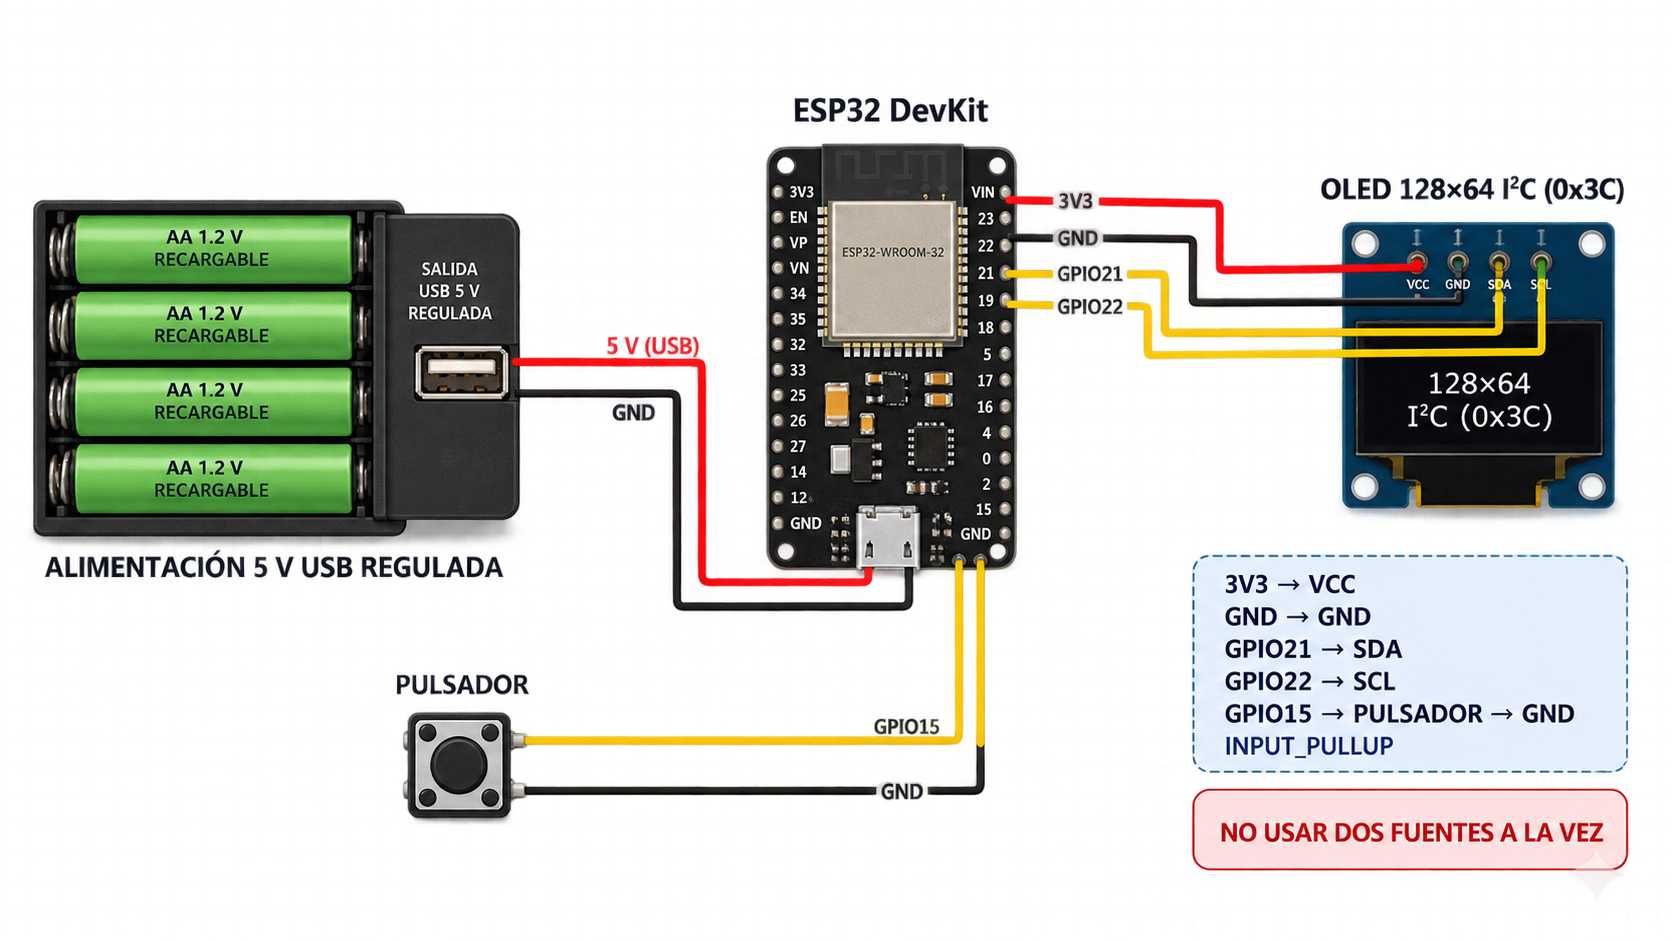
\includegraphics[width=0.98\linewidth]{figuras/diagrama-electronico-eilor}}
\caption{Diagrama funcional de conexiones y alimentación autónoma de EILOR. Los colores identifican alimentación positiva (rojo), tierra (negro) y señales (amarillo); la posición gráfica de los terminales no sustituye el pinout de la Tabla~\ref{tab:pinout}.}
\label{fig:esquematico}
\end{figure}

La figura fue generada con asistencia de inteligencia artificial y posteriormente
contrastada con el firmware del proyecto y la documentación del fabricante. La
verificación confirmó GPIO21 para SDA, GPIO22 para SCL y GPIO15 para el pulsador;
asimismo, la guía de la placa establece que USB, 5V/GND y 3V3/GND son alternativas
de alimentación mutuamente excluyentes \parencite{espressifdevkit2026}. Por ello,
debe utilizarse una sola fuente: en operación autónoma, un portapilas con salida
USB regulada a 5~V; durante programación, el USB del computador, desconectando
previamente el portapilas.

\section{Asignación de pines (pinout)}
La Tabla~\ref{tab:pinout} detalla las conexiones. El pulsador se conecta entre GPIO15 y GND; al configurarse la entrada como \code{INPUT\_PULLUP}, el pin se lee en alto en reposo y en bajo al pulsar, eliminando la necesidad de una resistencia externa.

\begin{table}[H]
\centering
\caption{Asignación de pines del ESP32}
\label{tab:pinout}
\footnotesize
\begin{tabularx}{\linewidth}{@{}l l l X@{}}
\toprule
\textbf{Pin ESP32} & \textbf{Señal} & \textbf{Componente} & \textbf{Notas} \\
\midrule
3V3 & Alimentación & OLED VCC & Lógica y alimentación a 3.3~V \\
GND & Común & OLED / Pulsador & Referencia de tierra compartida \\
GPIO21 & SDA (I\textsuperscript{2}C) & OLED & Datos del bus I\textsuperscript{2}C \\
GPIO22 & SCL (I\textsuperscript{2}C) & OLED & Reloj del bus I\textsuperscript{2}C \\
GPIO15 & Entrada digital & Pulsador & \code{INPUT\_PULLUP}; activo en bajo \\
\bottomrule
\end{tabularx}
\end{table}

\section{Lista de materiales (BOM)}
La Tabla~\ref{tab:bom} presenta la lista de materiales con un costo estimado referencial.

\begin{table}[H]
\centering
\caption{Lista de materiales y costo estimado}
\label{tab:bom}
\footnotesize
\begin{tabularx}{\linewidth}{@{}X c c c@{}}
\toprule
\textbf{Componente} & \textbf{Cant.} & \textbf{Costo unit. (USD)} & \textbf{Subtotal (USD)} \\
\midrule
Placa ESP32 DevKit (WROOM-32) & 1 & 6.50 & 6.50 \\
Pantalla OLED SSD1306 0.96" I\textsuperscript{2}C & 1 & 3.00 & 3.00 \\
Pulsador momentáneo & 1 & 0.20 & 0.20 \\
Protoboard y cables Dupont & 1 & 3.00 & 3.00 \\
Cable USB de alimentación & 1 & 1.50 & 1.50 \\
Portapilas 4\(\times\)AA con salida USB regulada a 5~V y pilas NiMH & 1 & 10.00 & 10.00 \\
\midrule
\multicolumn{3}{r}{\textbf{Total estimado}} & \textbf{24.20} \\
\bottomrule
\end{tabularx}
\end{table}

\section{Diseño conceptual de la carcasa}

La Figura~\ref{fig:carcasa-eilor} propone una carcasa de dos piezas imprimible en
3D. El diseño separa el portapilas de la electrónica, mantiene accesibles la
pantalla, el pulsador y el puerto USB, incorpora ventilación y reserva una zona
sin metal frente a la antena impresa del ESP32. Los postes de montaje y canales
internos inmovilizan las placas y reducen esfuerzos sobre los conductores.

\begin{figure}[H]
\centering
\setlength{\fboxsep}{0pt}\setlength{\fboxrule}{0.4pt}%
\fcolorbox{gray!45}{white}{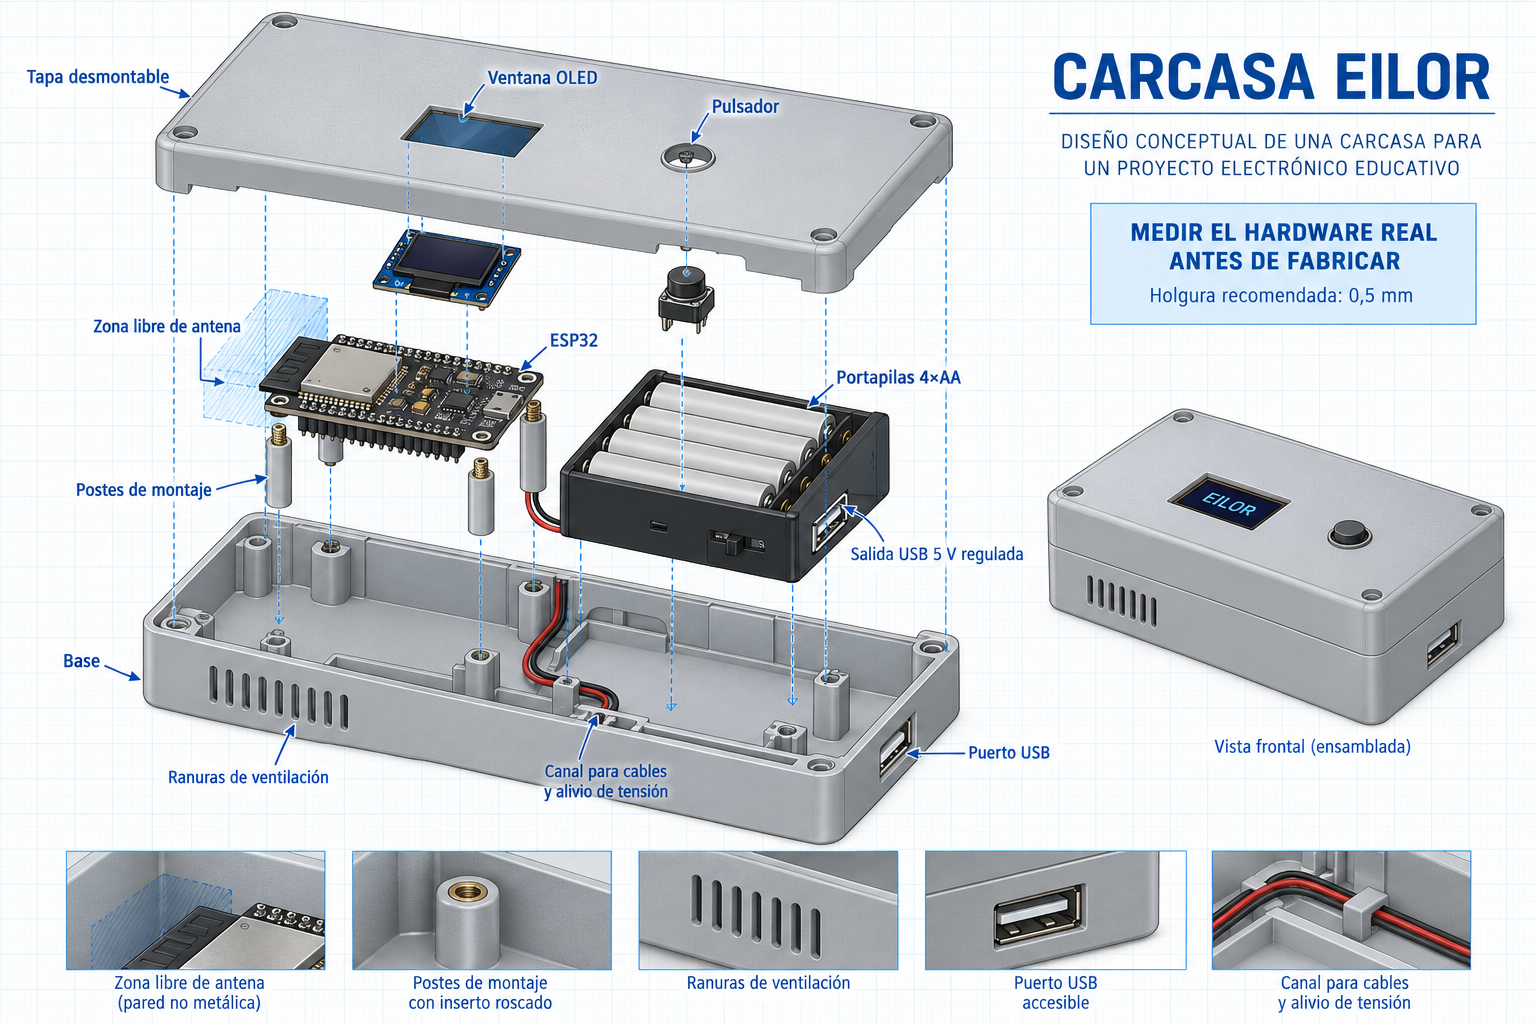
\includegraphics[width=0.98\linewidth]{figuras/carcasa-eilor-conceptual}}
\caption{Propuesta conceptual de carcasa para EILOR con compartimento de pilas, acceso a USB y zona libre frente a la antena.}
\label{fig:carcasa-eilor}
\end{figure}

La imagen de carcasa es una referencia de distribución, no un plano listo para
fabricación. Antes de modelar el archivo STL deben medirse con calibrador la placa,
la OLED, el pulsador, el portapilas y la posición exacta de conectores y orificios.
Se recomienda una holgura inicial de 0.5~mm por lado, prototipar primero la base y
confirmar que ningún poste, tornillo o cable invada la zona de la antena.

\section{Consideraciones de alimentación y coexistencia RF}
El consumo del ESP32 durante el escaneo activo con ambas radios puede presentar picos de corriente; por ello se recomienda alimentación regulada de 5~V por USB capaz de entregar al menos 500~mA. Las pilas AA no se conectan directamente a 3V3 ni a 5V: el portapilas debe integrar una salida USB regulada. En el firmware se habilita \code{WiFi.setSleep(true)} para favorecer la \emph{coexistencia} temporal entre Wi\nobreakdash-Fi y BLE, que comparten la misma radio de 2.4~GHz, evitando la inanición de una tecnología por la otra. La captura fotográfica del montaje físico se incorpora en el Anexo correspondiente.

\captura[0.85]{foto-montaje-monitor-serie}{Montaje físico del prototipo (ESP32 + OLED sobre \emph{protoboard}) y monitor serie durante la puesta en marcha.}

%============================ BASE DE DATOS (ENTREGA 2) =====================
\chapter{Diseño de la base de datos}
\label{cap:basedatos}

\section{Estrategia de persistencia}
Por decisión de diseño ---priorizando la portabilidad, la ausencia de dependencias nativas y la facilidad de despliegue en cualquier entorno, incluida la nube--- EILOR implementa su capa de datos mediante \emph{persistencia en archivos JSON} gestionada por el módulo \code{lib/store}. Esta aproximación, adecuada para el volumen y la naturaleza del prototipo, se comporta como una base de datos documental ligera: cada colección se materializa en un archivo, con escritura atómica mediante archivo temporal y renombrado. La Sección~\ref{sec:migracion} describe la ruta de migración a un motor relacional para escenarios de mayor escala.

\section{Modelo entidad-relación}
La Figura~\ref{fig:er} presenta el modelo conceptual. Las entidades \textbf{Dispositivo}, \textbf{MuestraTemporal} y \textbf{Registro} son independientes en el modelo documental actual, pero se relacionan lógicamente con la entidad \textbf{PuntoAcceso} (el SoftAP activo) y con la sesión de captura.

\begin{figure}[H]
\centering
\begin{tikzpicture}[
  ent/.style={rectangle,draw,very thick,rounded corners=2pt,align=center,
              minimum width=3.0cm,minimum height=1.0cm,fill=eilorcyan!8,font=\small},
  rel/.style={diamond,aspect=1.6,draw,thick,align=center,font=\scriptsize,fill=eiloremerald!10,inner sep=1pt},
  arr/.style={-{Latex[length=2mm]},thick},
  attr/.style={font=\scriptsize\itshape,align=center}
]
\node[ent] (dev) {Dispositivo};
\node[ent,right=3.2cm of dev] (ap) {PuntoAcceso (SoftAP)};
\node[ent,below=2.0cm of dev] (ts) {MuestraTemporal};
\node[ent,below=2.0cm of ap] (reg) {Registro (invitado)};

\node[rel] (r1) at ($(dev)!0.5!(ap)$) {detecta};
\node[rel] (r2) at ($(ap)!0.5!(reg)$) {genera};

\draw[arr] (dev) -- (r1); \draw[arr] (r1) -- (ap);
\draw[arr] (ap) -- (r2); \draw[arr] (r2) -- (reg);
\draw[arr,dashed] (dev) -- node[attr,left]{agrega} (ts);

\node[attr,above=0.1cm of dev] {mac (PK), rssi, channel, vendor, evilTwin};
\node[attr,above=0.1cm of ap] {apSsid, apChannel, apActive};
\node[attr,below=0.1cm of ts] {t (PK), wifi, ble, active, rate};
\node[attr,below=0.1cm of reg] {id (PK), nombre, apellido, telefono, ts};
\end{tikzpicture}
\caption{Modelo entidad-relación conceptual de EILOR.}
\label{fig:er}
\end{figure}

\section{Esquema físico (archivos JSON)}
El módulo \code{lib/store} define tres archivos bajo el directorio \code{data/}, descritos en la Tabla~\ref{tab:archivos}.

\begin{table}[H]
\centering
\caption{Archivos de persistencia}
\label{tab:archivos}
\footnotesize
\begin{tabularx}{\linewidth}{@{}l l X@{}}
\toprule
\textbf{Archivo} & \textbf{Estructura} & \textbf{Contenido / política} \\
\midrule
\code{state.json} & Objeto & Instantánea de dispositivos y total de paquetes; \emph{snapshot} cada 30~s \\
\code{timeseries.json} & Arreglo & Muestras por minuto; retención máx. 720 (\code{MAX\_TIMESERIES}) \\
\code{registrations.json} & Arreglo & Altas de invitados; retención máx. 5000 (\code{MAX\_REGISTRATIONS}) \\
\bottomrule
\end{tabularx}
\end{table}

El Listado~\ref{lst:store} muestra la escritura atómica y el modelo de retención de la serie temporal.

\begin{lstlisting}[style=js,caption={Escritura atómica y retención (lib/store.js)},label={lst:store}]
function saveJSON(file, data) {
  try {
    ensureDir();
    const tmp = file + '.tmp';                 // escritura atomica:
    fs.writeFileSync(tmp, JSON.stringify(data)); // 1) escribe temporal
    fs.renameSync(tmp, file);                   // 2) renombra (atomico)
    return true;
  } catch (e) { return false; }
}

function saveTimeseries(series) {
  return saveJSON(HISTORY_FILE, series.slice(-MAX_TIMESERIES)); // retencion
}
\end{lstlisting}

\subsection{Ejemplo de documento (registro de invitado)}
\begin{lstlisting}[style=json,caption={Documento de la colección registrations.json}]
{
  "id": "mudcvuhsnl34",
  "nombre": "Maria",
  "apellido": "Perez",
  "telefono": "099 123 4567",
  "apSsid": "Cafe-EILOR",
  "source": "esp32",
  "ts": 1790121584629
}
\end{lstlisting}

\section{Ruta de migración a base de datos relacional}
\label{sec:migracion}
Para escenarios multi\nobreakdash-dispositivo o de retención prolongada se propone migrar a un motor relacional (SQLite en despliegues embebidos o PostgreSQL en la nube). El Listado~\ref{lst:sql} presenta el esquema relacional equivalente, que preserva las entidades del modelo ER y agrega integridad referencial e índices para consultas eficientes.

\begin{lstlisting}[language=SQL,caption={Esquema relacional propuesto},label={lst:sql},basicstyle=\ttfamily\footnotesize,keywordstyle=\color{codekw}\bfseries]
CREATE TABLE dispositivo (
  mac         VARCHAR(32) PRIMARY KEY,
  tipo        VARCHAR(8)  NOT NULL,   -- 'wifi' | 'ble'
  ssid        VARCHAR(64),
  rssi        INTEGER,
  channel     INTEGER,
  vendor      VARCHAR(64),
  random_mac  BOOLEAN DEFAULT FALSE,
  evil_twin   BOOLEAN DEFAULT FALSE,
  last_seen   BIGINT
);

CREATE TABLE registro (
  id        VARCHAR(24) PRIMARY KEY,
  nombre    VARCHAR(60) NOT NULL,
  apellido  VARCHAR(60),
  telefono  VARCHAR(30),
  ap_ssid   VARCHAR(40),
  fuente    VARCHAR(16),
  ts        BIGINT NOT NULL
);
CREATE INDEX idx_registro_ts ON registro (ts);

CREATE TABLE muestra_temporal (
  t        BIGINT PRIMARY KEY,
  wifi     INTEGER, ble INTEGER,
  activos  INTEGER, paquetes BIGINT, tasa INTEGER
);
\end{lstlisting}

Esta migración es transparente para el resto del sistema gracias al desacoplamiento que ofrece \code{lib/store}: bastaría reimplementar sus funciones (\code{loadDevices}, \code{saveDevices}, \code{loadTimeseries}, \code{saveTimeseries}, \code{loadRegistrations}, \code{saveRegistrations}) sobre el nuevo motor, sin alterar \code{server.js}.

%============================ IMPLEMENTACIÓN (ENTREGA 2) ====================
\chapter{Implementación del prototipo}
\label{cap:implementacion}

Este capítulo documenta la implementación real del sistema. El proyecto suma más de 3\,900 líneas de código distribuidas entre el firmware del ESP32 (777 líneas), el servidor Node.js (665 líneas más 274 en los módulos \code{lib/}) y el frontend (913 líneas de lógica, 419 de estructura y 1\,272 de estilos). Se presentan los fragmentos más representativos; los archivos completos se referencian en los anexos y se acompañan de capturas donde procede.

\section{Programación del firmware (Arduino / ESP32)}
El firmware se desarrolló en C++ sobre el \emph{core} de Arduino para ESP32, empleando las librerías \code{WiFi}, \code{WebServer}, \code{DNSServer}, \code{WebSocketsClient} (Markus Sattler), la pila BLE nativa y \code{Adafruit\_SSD1306} para la pantalla. El bucle principal coordina el escaneo, el \emph{heartbeat}, la lectura del pulsador y, en modo SoftAP, la atención del portal cautivo.

\subsection{Estructura de modos y bucle principal}
El Listado~\ref{lst:loop} muestra el despacho por modo dentro de \code{loop()}.

\begin{lstlisting}[style=cpp,caption={Bucle principal y despacho por modo (firmware)},label={lst:loop}]
void loop() {
  webSocket.loop();
  button.loop();

  // Heartbeat cada 3 s hacia el servidor
  if (isWsConnected && (millis() - lastHeartbeatTime > 3000)) {
    webSocket.sendTXT("{\"action\":\"heartbeat\"" + tokenField() + ...);
    lastHeartbeatTime = millis();
  }
  if (button.isPressed()) applyMode((current_mode + 1) % 4); // pulsador D15

  switch (current_mode) {
    case 0: if (millis() - lastScanTime > 3000) { scanAndAnalyzeSpectrum(); lastScanTime = millis(); } break;
    case 1: if (millis() - lastScanTime > 3000) { scanAndStreamBLE();      lastScanTime = millis(); } break;
    case 2: if (captiveRunning) { dnsServer.processNextRequest(); captiveServer.handleClient(); } break;
    case 3: break; // standby
  }
}
\end{lstlisting}

El cambio de modo se realiza físicamente con el pulsador (GPIO15); en cada
pulsación el firmware avanza al siguiente modo y refresca la pantalla OLED con la
información propia de ese estado. Las Figuras siguientes muestran el dispositivo
físico operando en los modos de escaneo Wi\nobreakdash-Fi y BLE.

\captura[0.7]{foto-oled-wifi}{Pantalla OLED en modo escaneo Wi\nobreakdash-Fi (modo 0): total de redes, canal más saturado y canal recomendado.}

\captura[0.7]{foto-oled-ble}{Pantalla OLED en modo escaneo BLE (modo 1): dispositivos detectados y RSSI del más cercano.}

\subsection{Escaneo de espectro Wi-Fi}
En el modo 0, el firmware realiza un escaneo asíncrono, cuenta los puntos de acceso por canal y construye una trama JSON con los dispositivos y el histograma de canales, que envía por WebSocket (Listado~\ref{lst:scan}).

\begin{lstlisting}[style=cpp,caption={Escaneo y serialización del espectro Wi-Fi},label={lst:scan}]
String json = "{\"type\":\"spectrum_wifi\"" + tokenField() +
              ",\"deviceId\":\"ESP32-EILOR\",\"devices\":[";
for (int i = 0; i < n; ++i) {
  int ch = WiFi.channel(i);
  if (ch >= 1 && ch <= 13) channelCounts[ch]++;
  if (i > 0) json += ",";
  json += "{\"ssid\":\""   + WiFi.SSID(i)     + "\","
          "\"bssid\":\""   + WiFi.BSSIDstr(i) + "\","
          "\"rssi\":"      + String(WiFi.RSSI(i))    + ","
          "\"channel\":"   + String(ch)              + "}";
}
json += "],\"channels\":{ ... }}";
if (isWsConnected) webSocket.sendTXT(json);
\end{lstlisting}

\subsection{Portal cautivo y \emph{buffer} offline}
Al entrar en modo SoftAP, \code{startCaptivePortal()} inicia un servidor DNS que redirige todas las consultas a la IP del ESP32 y un servidor HTTP que sirve el formulario. El manejador del formulario delega en \code{queueOrSendReg()}, que envía el registro o lo encola si no hay enlace (Listado~\ref{lst:buffer}).

\begin{lstlisting}[style=cpp,caption={Envío con buffer offline (firmware)},label={lst:buffer}]
void queueOrSendReg(const String& nombre, const String& apellido,
                    const String& telefono, const String& apSsid) {
  if (isWsConnected) {
    String j = buildRegJson(nombre, apellido, telefono, apSsid); // local (sendTXT pide String&)
    webSocket.sendTXT(j);
  } else if (pendingCount < MAX_PENDING) {          // sin enlace: encolar
    pendingRegs[pendingCount++] = { nombre, apellido, telefono, apSsid };
  }
}
void flushPendingRegs() {                            // al reconectar: reenviar
  if (!isWsConnected || pendingCount == 0) return;
  for (int i = 0; i < pendingCount; i++) {
    String j = buildRegJson(pendingRegs[i].nombre, pendingRegs[i].apellido,
                            pendingRegs[i].telefono, pendingRegs[i].apSsid);
    webSocket.sendTXT(j); delay(30);
  }
  pendingCount = 0;
}
\end{lstlisting}

\captura[0.7]{foto-oled-softap}{Pantalla OLED en modo SoftAP: SSID emitido, canal, IP del portal (192.168.4.1) y contadores de clientes y registros.}

\section{Implementación del servidor (Node.js)}
\subsection{Módulo de análisis de canales}
El corazón analítico es \code{analyzeChannels()}, que calcula un puntaje de interferencia por canal ponderando el solapamiento de canales adyacentes (hasta 4 canales de distancia) y la intensidad de señal, y recomienda el canal más limpio del conjunto no solapado (Listado~\ref{lst:analysis}).

\begin{lstlisting}[style=js,caption={Puntaje de interferencia por canal (lib/analysis.js)},label={lst:analysis}]
function analyzeChannels(wifiHeatmap) {
  const scores = {};
  for (let ch = 1; ch <= 13; ch++) {
    let score = 0;
    for (let other = 1; other <= 13; other++) {
      const data = wifiHeatmap[other];
      if (!data || !data.count) continue;
      const dist = Math.abs(ch - other);
      if (dist > 4) continue;                        // sin solapamiento significativo
      const overlapWeight = 1 - dist / 5;            // decae con la distancia
      const rssiWeight = Math.max(0.2, Math.min(1, (data.maxRssi + 95) / 55));
      score += data.count * overlapWeight * rssiWeight;
    }
    scores[ch] = Math.round(score * 10) / 10;
  }
  // ... determina bestChannel, worstChannel y recommendedChannel (1/6/11)
  return { scores, bestChannel, worstChannel, recommendedChannel };
}
\end{lstlisting}

\subsection{Detección de gemelo malicioso}
La heurística agrupa por SSID y marca como sospechosos los que aparecen bajo más de un BSSID (Listado~\ref{lst:evil}).

\begin{lstlisting}[style=js,caption={Detección de evil twin (lib/analysis.js)},label={lst:evil}]
function detectEvilTwins(devices) {
  const bySsid = new Map();
  devices.forEach(d => {
    if (d.type !== 'wifi') return;
    const ssid = (d.ssid || '').trim();
    if (!ssid || ssid === 'Oculto') return;
    if (!bySsid.has(ssid)) bySsid.set(ssid, new Set());
    bySsid.get(ssid).add((d.mac || '').toLowerCase());
  });
  const flagged = new Set();
  bySsid.forEach(macs => { if (macs.size > 1) macs.forEach(m => flagged.add(m)); });
  return flagged;                                    // BSSIDs bajo el mismo SSID
}
\end{lstlisting}

\subsection{Identificación de fabricante (OUI)}
El módulo \code{lib/oui} mantiene un catálogo de 123 prefijos y detecta MAC aleatorizadas por el segundo \emph{nibble} del primer octeto (Listado~\ref{lst:oui}).

\begin{lstlisting}[style=js,caption={Búsqueda de fabricante y MAC aleatoria (lib/oui.js)},label={lst:oui}]
function lookupVendor(mac) {
  const clean = normalizeMac(mac);
  const prefix = clean.slice(0, 6);
  if (OUI_MAP[prefix]) return OUI_MAP[prefix];
  const secondNibble = clean[1];                     // MAC localmente administrada
  if (['2','6','A','E'].includes(secondNibble)) return 'MAC Aleatoria (privacidad)';
  return 'Desconocido';
}
\end{lstlisting}

\subsection{Autenticación por token}
El módulo \code{lib/auth} implementa sesiones por token con expiración y un \emph{middleware} \code{requireAuth} para proteger las rutas de control, además de \code{deviceAuthorized} para la ingesta (Listado~\ref{lst:auth}).

\begin{lstlisting}[style=js,caption={Sesiones y middleware de autorización (lib/auth.js)},label={lst:auth}]
function login(password) {
  if (password !== PASSWORD) return null;
  const token = crypto.randomBytes(24).toString('hex');
  tokens.set(token, Date.now() + TTL_MS);            // TTL 24 h
  return token;
}
function requireAuth(req, res, next) {
  const token = req.headers['x-eilor-token'] || req.query.token || (req.body && req.body.token);
  if (isValidToken(token)) return next();
  return res.status(401).json({ error: 'No autorizado. Inicia sesion.' });
}
function deviceAuthorized(t) { return !DEVICE_TOKEN || t === DEVICE_TOKEN; }
\end{lstlisting}

\subsection{Ingesta y difusión en tiempo real}
Al recibir un escaneo, \code{server.js} anota cada dispositivo con fabricante, MAC aleatoria y bandera de gemelo malicioso, recalcula el mapa de calor y difunde el resultado a los clientes (Listado~\ref{lst:ingest}).

\begin{lstlisting}[style=js,caption={Anotación y difusión (server.js)},label={lst:ingest}]
function annotateDevices(list) {
  return list.map(dev => ({
    ...dev,
    vendor: dev.vendor || lookupVendor(dev.mac),
    randomMac: dev.randomMac !== undefined ? dev.randomMac : isRandomMac(dev.mac),
    evilTwin: evilTwinMacs.has((dev.mac || '').toLowerCase())
  }));
}
// tras procesar el lote:
broadcast({ event: 'scan_update', heatmap: channelHeatmap,
            latestBatch: annotateDevices(Array.from(activeDevices.values())) });
\end{lstlisting}

\section{Implementación del frontend (dashboard)}
El cliente web establece la conexión WebSocket, solicita el estado inicial y despacha los eventos entrantes hacia los distintos renderizadores (mapa de calor, radar, tabla de dispositivos, registros y serie temporal). El Listado~\ref{lst:front} ilustra el manejo del evento de escaneo.

\begin{lstlisting}[style=js,caption={Manejo de eventos en el cliente (public/app.js)},label={lst:front}]
if (data.event === 'initial_state' || data.event === 'scan_update') {
  if (data.latestBatch) state.devices = data.latestBatch;
  if (data.heatmap)    { state.heatmap = data.heatmap; renderHeatmap(data.heatmap); }
  renderDevicesTable();
  renderRadarBlips();
  updateCounters();
}
\end{lstlisting}

\captura[0.98]{cap-espectro-radar}{Dashboard web en operación: mapa de saturación espectral Wi\nobreakdash-Fi (canales 1--13) y radar de proximidad BLE, alimentados en vivo por WebSocket.}

%============================ CLOUDFLARE / SAAS (ENTREGA 2) =================
\chapter{Despliegue SaaS en la nube con Cloudflare}
\label{cap:cloudflare}

\section{Modelo de entrega como servicio (SaaS)}
EILOR se entrega bajo un modelo \emph{Software as a Service}: el servidor Node.js se ejecuta de forma continua y se publica en Internet mediante un \emph{túnel} de Cloudflare, de modo que tanto el dispositivo ESP32 como los clientes web acceden al sistema a través de un nombre de dominio público con cifrado TLS, sin exponer directamente la máquina ni abrir puertos entrantes en la red local. En la implementación de referencia, el sistema se publica en el dominio \code{esp.orellanadigitalco.trade} sobre el puerto 443 (WSS/HTTPS).

\section{Arquitectura del túnel}
Cloudflare Tunnel (\code{cloudflared}) establece una conexión saliente y persistente desde el servidor de origen hacia la red perimetral (\emph{edge}) de Cloudflare. El tráfico de los usuarios llega primero al \emph{edge}, donde se termina el TLS, y desde allí viaja por el túnel hasta el servidor local. La Figura~\ref{fig:cloudflare} ilustra el modelo.

\begin{figure}[H]
\centering
\begin{tikzpicture}[
  font=\small,
  n/.style={rectangle,rounded corners=3pt,draw,thick,align=center,minimum height=1.0cm,minimum width=2.6cm},
  arr/.style={-{Latex[length=2.4mm]},thick},
  lbl/.style={font=\scriptsize\itshape,align=center}
]
\node[n,fill=eilorcyan!10] (esp) {ESP32};
\node[n,fill=gray!8,below=0.8cm of esp] (web) {Navegador\\/ Invitado};
\node[n,fill=orange!14,right=2.6cm of esp,yshift=-0.7cm,minimum height=1.8cm] (edge) {Cloudflare\\Edge\\(TLS 443)};
\node[n,fill=yellow!14,right=2.4cm of edge] (cfd) {cloudflared\\(túnel saliente)};
\node[n,fill=eiloremerald!12,right=2.2cm of cfd] (srv) {Node.js\\:3002 (PM2)};

\draw[arr] (esp) -- node[lbl,above]{WSS} (edge);
\draw[arr] (web) -- node[lbl,below]{HTTPS} (edge);
\draw[{Latex[length=2.4mm]}-{Latex[length=2.4mm]},thick] (edge) -- node[lbl,above]{túnel\\cifrado} (cfd);
\draw[arr] (cfd) -- node[lbl,above]{HTTP\\local} (srv);
\end{tikzpicture}
\caption{Publicación del servidor mediante Cloudflare Tunnel.}
\label{fig:cloudflare}
\end{figure}

\section{Ventajas de seguridad}
\begin{itemize}[leftmargin=1.4em]
  \item \textbf{Sin puertos entrantes:} el origen no expone puertos; el túnel es una conexión saliente, lo que reduce la superficie de ataque.
  \item \textbf{TLS gestionado:} el certificado y la terminación TLS los administra Cloudflare, garantizando cifrado extremo para WSS y HTTPS.
  \item \textbf{Ocultamiento de IP:} la dirección real del servidor no se publica en el DNS.
  \item \textbf{Controles de borde:} posibilidad de aplicar reglas de firewall, limitación de tasa y protección frente a denegación de servicio en el \emph{edge}.
\end{itemize}

\section{Configuración de referencia}
El Listado~\ref{lst:cfd} muestra una configuración típica de \code{cloudflared} con reglas de \emph{ingress} que enrutan el hostname público al servidor local, habilitando explícitamente WebSocket.

\begin{lstlisting}[caption={Configuración de Cloudflare Tunnel (config.yml)},label={lst:cfd},basicstyle=\ttfamily\footnotesize]
tunnel: eilor-tunnel
credentials-file: /home/saul/.cloudflared/<UUID>.json

ingress:
  - hostname: esp.orellanadigitalco.trade
    service: http://localhost:3002
    originRequest:
      noTLSVerify: true
      # WebSocket queda habilitado por defecto en cloudflared
  - service: http_status:404
\end{lstlisting}

El registro DNS asociado es un \code{CNAME} del hostname público hacia \code{<UUID>.cfargotunnel.com}, creado automáticamente por \code{cloudflared tunnel route dns}. Del lado del firmware, la conexión se establece con TLS mediante \code{webSocket.beginSSL(WS\_SERVER\_HOST, 443, "/")}, coherente con la terminación TLS en el \emph{edge}.

\section{Gestión del proceso con PM2}
El servidor se ejecuta bajo el gestor de procesos PM2, que garantiza su reinicio automático ante fallos y su arranque tras un reinicio del sistema operativo. El Listado~\ref{lst:pm2} resume los comandos de operación empleados.

\begin{lstlisting}[style=bash,caption={Operación del servicio con PM2},label={lst:pm2},basicstyle=\ttfamily\footnotesize]
pm2 start server.js --name eilor   # registrar el servicio
pm2 restart eilor --update-env     # recargar tras cambios de codigo
pm2 save                           # persistir para arranque automatico
pm2 logs eilor --lines 20          # inspeccionar registros
\end{lstlisting}

En conjunto, Cloudflare Tunnel y PM2 conforman la capa de \emph{entrega y operación} del SaaS: alta disponibilidad del proceso, publicación segura sin exposición directa y acceso cifrado uniforme para el hardware y los usuarios.

%============================ PLATAFORMA WEB (ENTREGA 2) ====================
\chapter{Plataforma web: interfaz, uso y comunicación}
\label{cap:plataforma}

Este capítulo documenta la plataforma de análisis y control de EILOR desde la
perspectiva de su uso: cómo se ingresa, qué opciones ofrece, cómo está construida
su interfaz y de qué manera se comunica con el dispositivo ESP32. La instancia de
referencia se encuentra publicada en \plataformaurl, servida a través del túnel de
Cloudflare descrito en el Capítulo~\ref{cap:cloudflare}.

\section{Acceso a la plataforma}
La plataforma se abre desde cualquier navegador moderno en la dirección pública
\plataformaurl{} o, en despliegues locales, en \code{http://localhost:3002}. Al
cargar, el \emph{dashboard} muestra de inmediato ---en modo de \emph{solo
lectura}--- el estado del ESP32, el modo activo, los contadores de dispositivos y
paquetes, el mapa de saturación espectral y el radar BLE, sin exigir credenciales.
Este acceso público de solo lectura permite observar el espectro sin poder emitir
comandos.

\subsection{Inicio de sesión}
Para habilitar las \emph{acciones de control} ---cambiar de modo, desplegar el
SoftAP, limpiar datos, listar o exportar registros--- se requiere iniciar sesión.
Al pulsar \emph{Iniciar Sesión} aparece el formulario de la Figura~\ref{fig:login},
que solicita la contraseña configurada en la variable de entorno
\code{EILOR\_PASSWORD}. Si la contraseña es correcta, el servidor emite un
\emph{token de sesión} (cadena hexadecimal de 48 caracteres, con vigencia de 24~h)
que el navegador conserva y adjunta en la cabecera \code{x-eilor-token} de cada
petición protegida. Una contraseña incorrecta devuelve \code{HTTP 401} y la sesión
no se habilita.

\begin{figure}[H]
\centering
\setlength{\fboxsep}{0pt}\setlength{\fboxrule}{0.4pt}%
\fcolorbox{gray!45}{white}{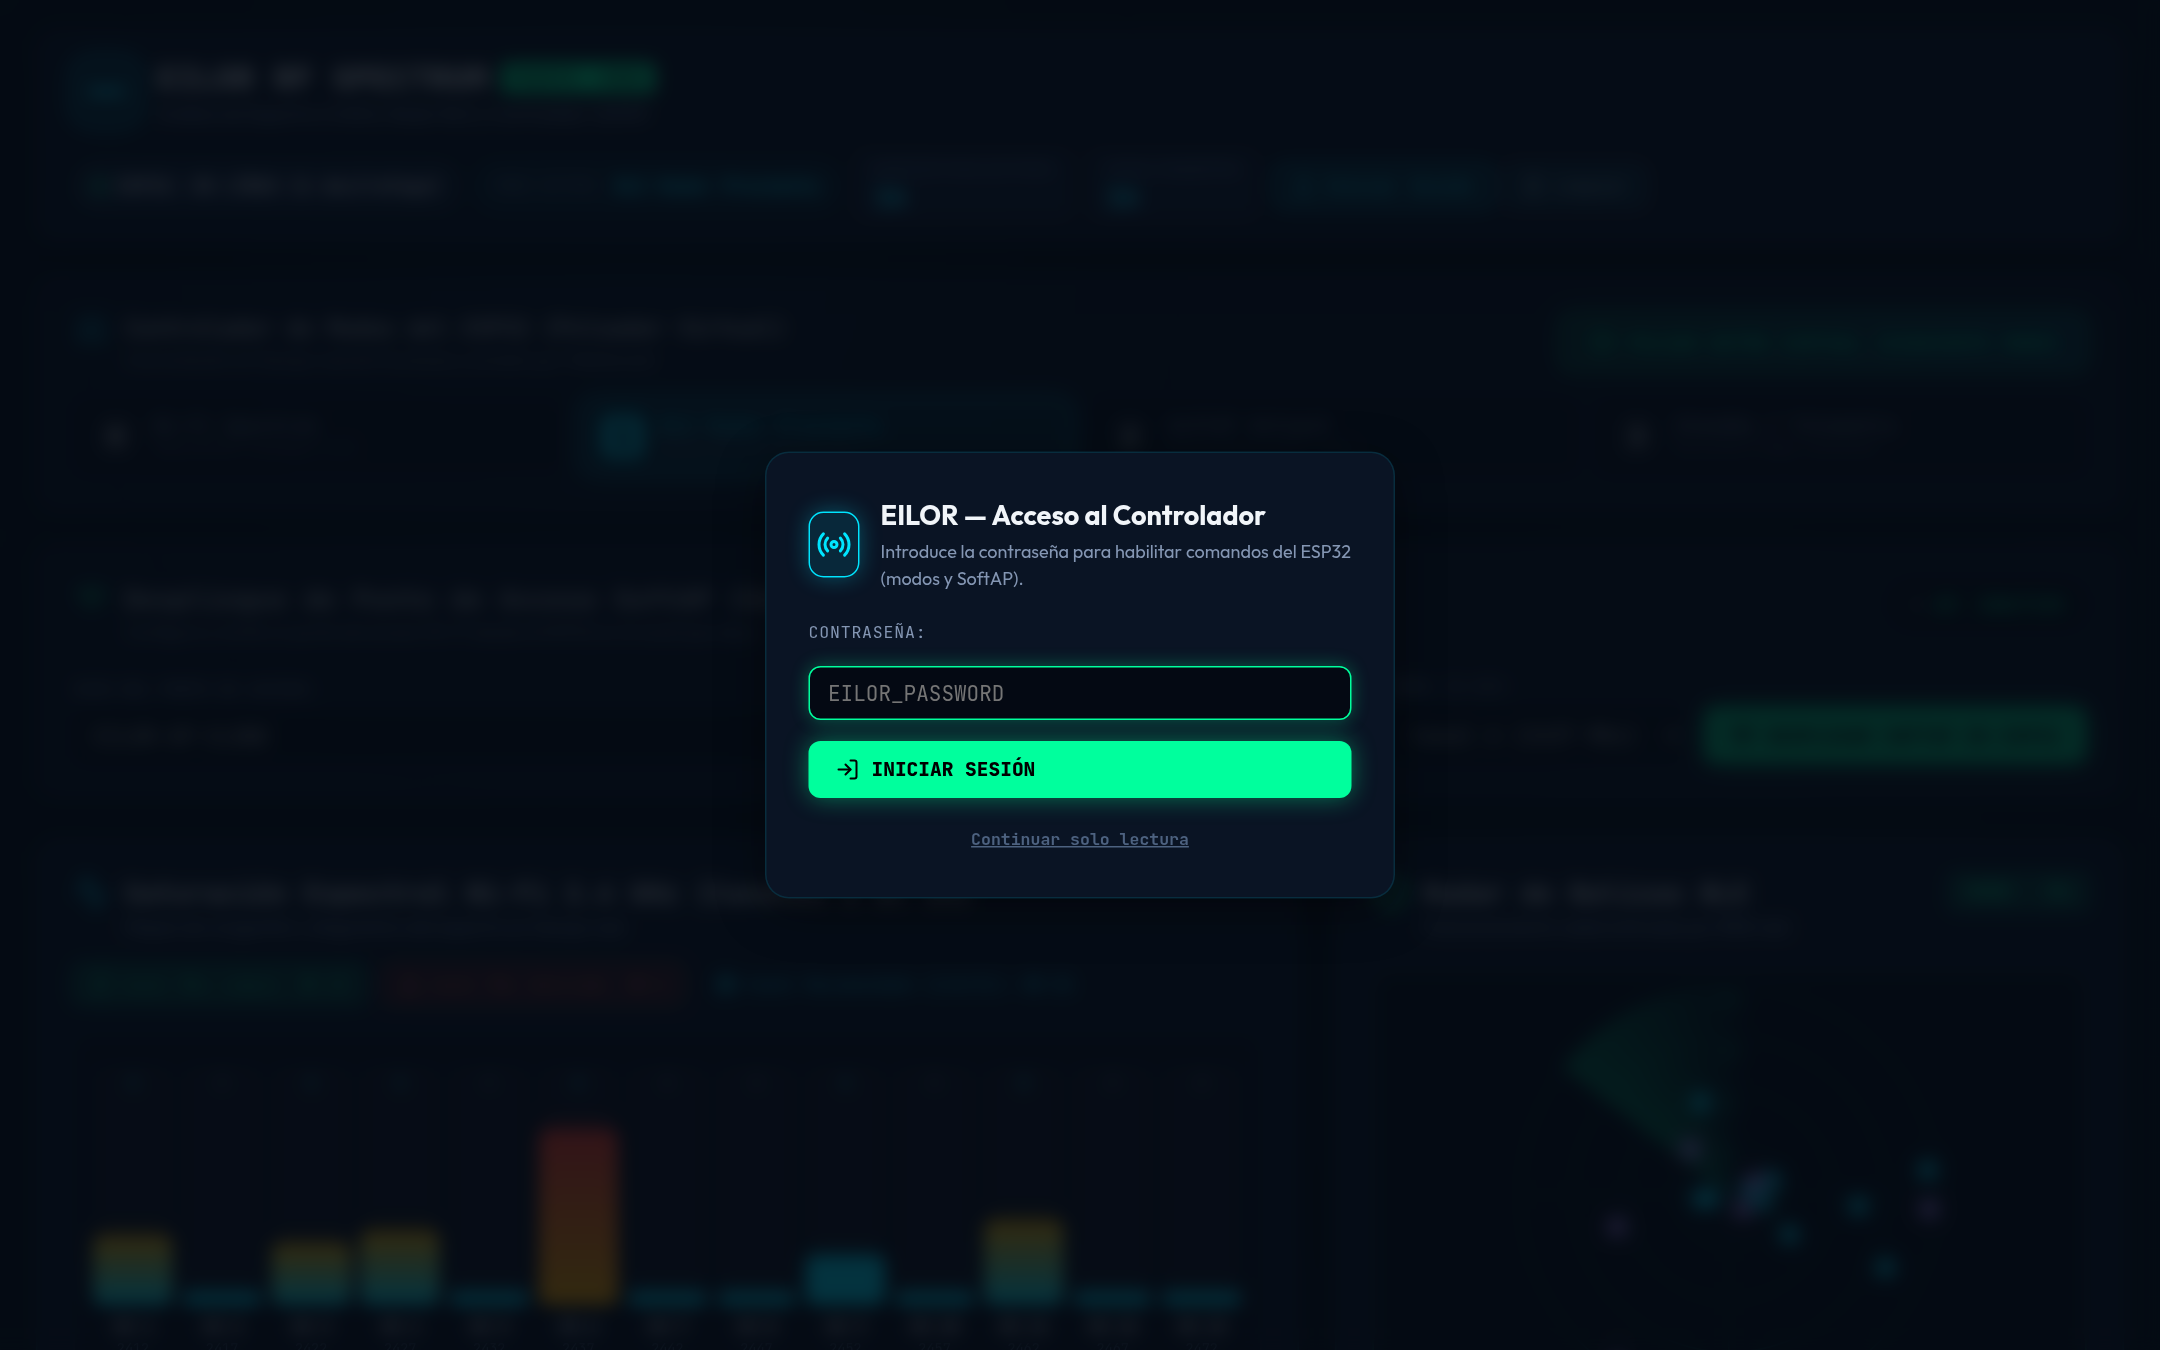
\includegraphics[width=0.78\linewidth]{figuras/cap-login}}
\caption{Formulario de inicio de sesión de la plataforma (habilita los comandos del ESP32).}
\label{fig:login}
\end{figure}

\section{Estructura y opciones de la interfaz}
El \emph{dashboard} organiza sus funciones en secciones apiladas verticalmente. La
Figura~\ref{fig:cabecera} muestra la cabecera de estado, con el indicador de
conexión del ESP32, el modo activo y los contadores globales, además de los botones
de sesión y de reinicio de datos.

\begin{figure}[H]
\centering
\setlength{\fboxsep}{0pt}\setlength{\fboxrule}{0.4pt}%
\fcolorbox{gray!45}{white}{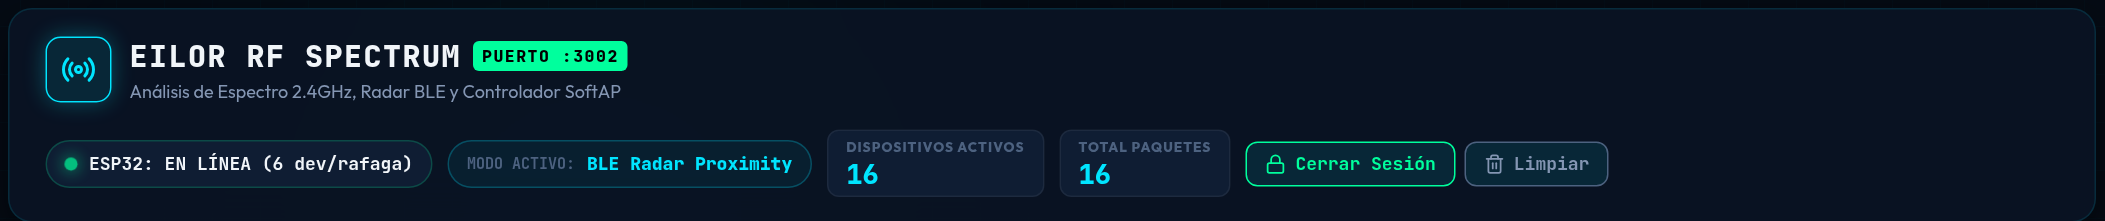
\includegraphics[width=0.98\linewidth]{figuras/cap-cabecera}}
\caption{Cabecera de estado: enlace del ESP32, modo activo y contadores de dispositivos y paquetes.}
\label{fig:cabecera}
\end{figure}

\subsection{Controlador de modos}
La sección \emph{Controlador de Modos} (Figura~\ref{fig:modos}) actúa como un
\emph{pulsador virtual}: replica en la web el botón físico del dispositivo. Permite
seleccionar directamente cualquiera de los cuatro modos ---(0)~Espectro Wi\nobreakdash-Fi,
(1)~Radar BLE, (2)~SoftAP con portal cautivo y (3)~Standby--- o avanzar al
siguiente. Cada cambio se emite por WebSocket y el ESP32 lo aplica en tiempo real.

\begin{figure}[H]
\centering
\setlength{\fboxsep}{0pt}\setlength{\fboxrule}{0.4pt}%
\fcolorbox{gray!45}{white}{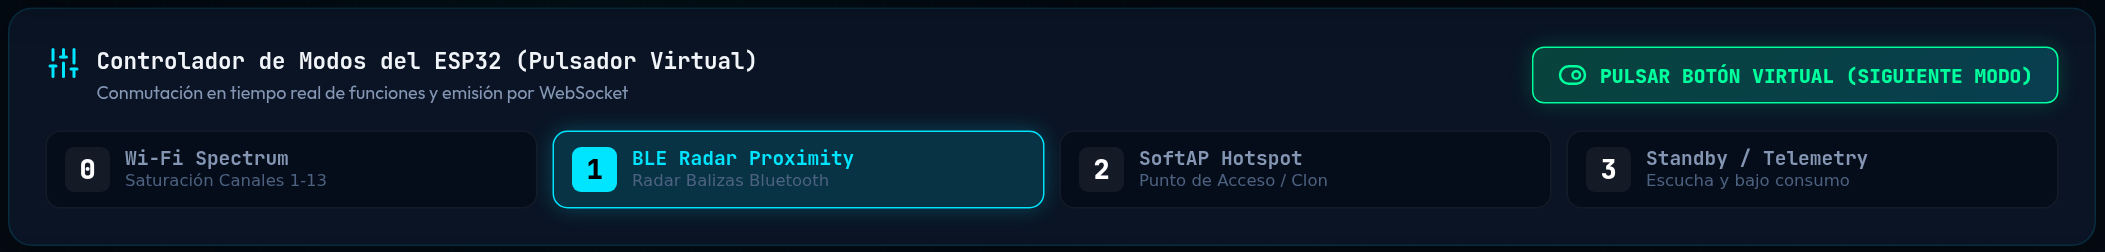
\includegraphics[width=0.98\linewidth]{figuras/cap-modos}}
\caption{Controlador de modos: conmutación remota de las cuatro funciones del ESP32.}
\label{fig:modos}
\end{figure}

\subsection{Despliegue del punto de acceso (SoftAP)}
En la sección \emph{Despliegue de Punto de Acceso} (Figura~\ref{fig:softap}) se
define el SSID y el canal (1--13) del punto de acceso propio y se pulsa
\emph{Desplegar SoftAP en ESP32}. El dispositivo pasa al modo~2, emite la red y
levanta el portal cautivo de registro. Esta funcionalidad está concebida
exclusivamente para redes propias, con un nombre identificable y aviso de registro,
conforme a las consideraciones éticas del Capítulo~\ref{cap:conclusiones}.

\begin{figure}[H]
\centering
\setlength{\fboxsep}{0pt}\setlength{\fboxrule}{0.4pt}%
\fcolorbox{gray!45}{white}{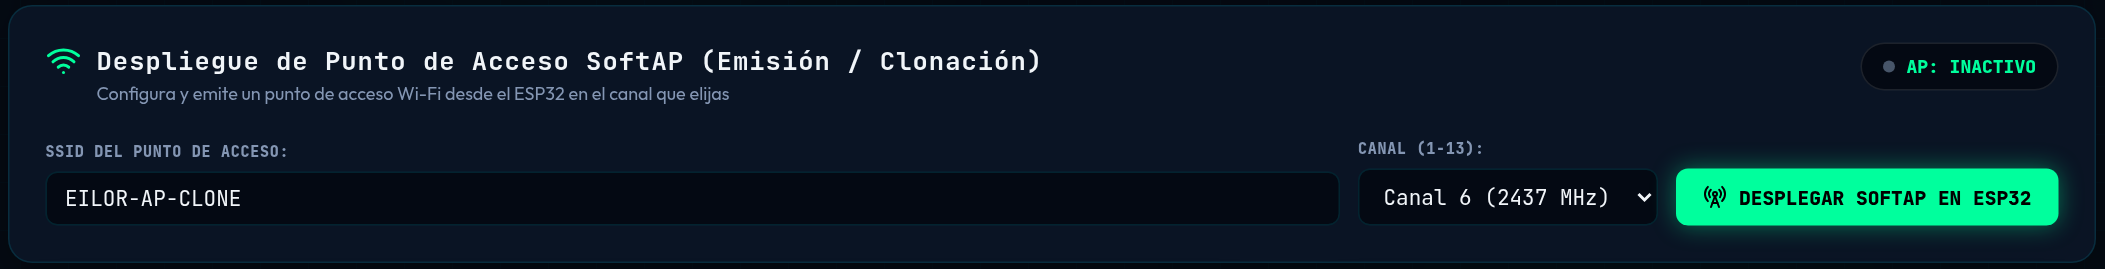
\includegraphics[width=0.98\linewidth]{figuras/cap-softap}}
\caption{Panel de despliegue del SoftAP: selección de SSID y canal del punto de acceso propio.}
\label{fig:softap}
\end{figure}

Cuando un invitado se conecta a la red emitida, su dispositivo es redirigido
automáticamente por el portal cautivo al formulario de registro
(Figura~\ref{fig:portal}), que solicita nombre, apellido y teléfono e incluye un
aviso explícito sobre la recolección de datos.

\begin{figure}[H]
\centering
\setlength{\fboxsep}{0pt}\setlength{\fboxrule}{0.4pt}%
\fcolorbox{gray!45}{white}{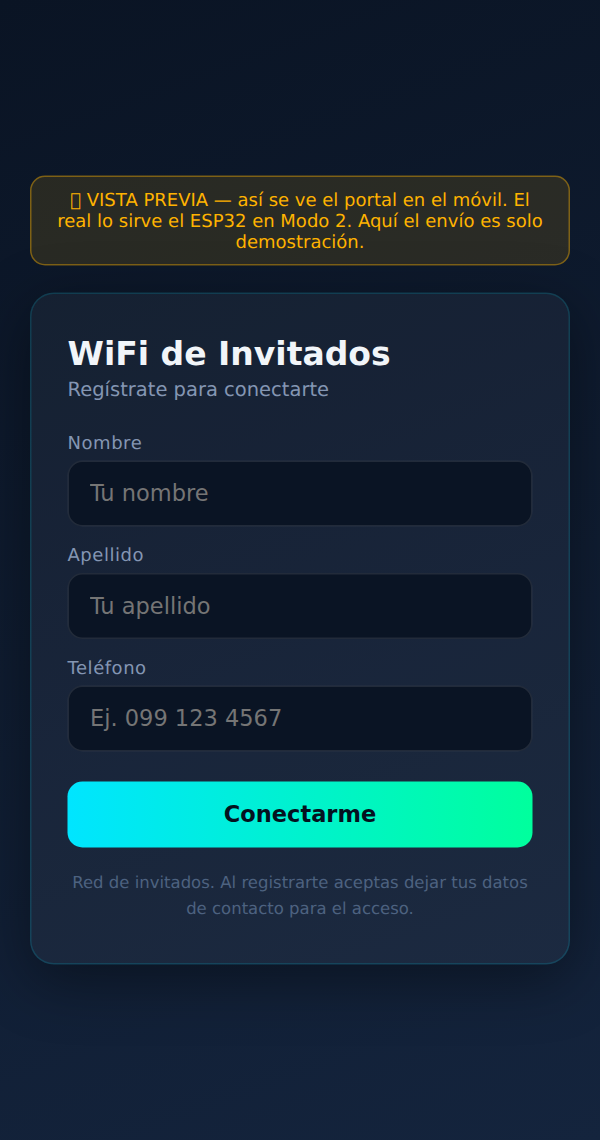
\includegraphics[height=8.5cm]{figuras/cap-portal}}
\caption{Formulario del portal cautivo tal como lo ve el invitado en su teléfono (vista previa).}
\label{fig:portal}
\end{figure}

\subsection{Análisis del espectro y radar BLE}
El núcleo analítico se visualiza en dos paneles contiguos
(Figura~\ref{fig:espectro-radar}): a la izquierda, el mapa de \emph{saturación
espectral} de los canales 1 al 13, con el canal más limpio, el más saturado y el
canal recomendado del conjunto no solapado 1/6/11; a la derecha, el \emph{radar de
proximidad BLE}, que ubica las balizas de forma radial según su RSSI. Ambos se
actualizan en vivo con cada ciclo de escaneo.

\begin{figure}[H]
\centering
\setlength{\fboxsep}{0pt}\setlength{\fboxrule}{0.4pt}%
\fcolorbox{gray!45}{white}{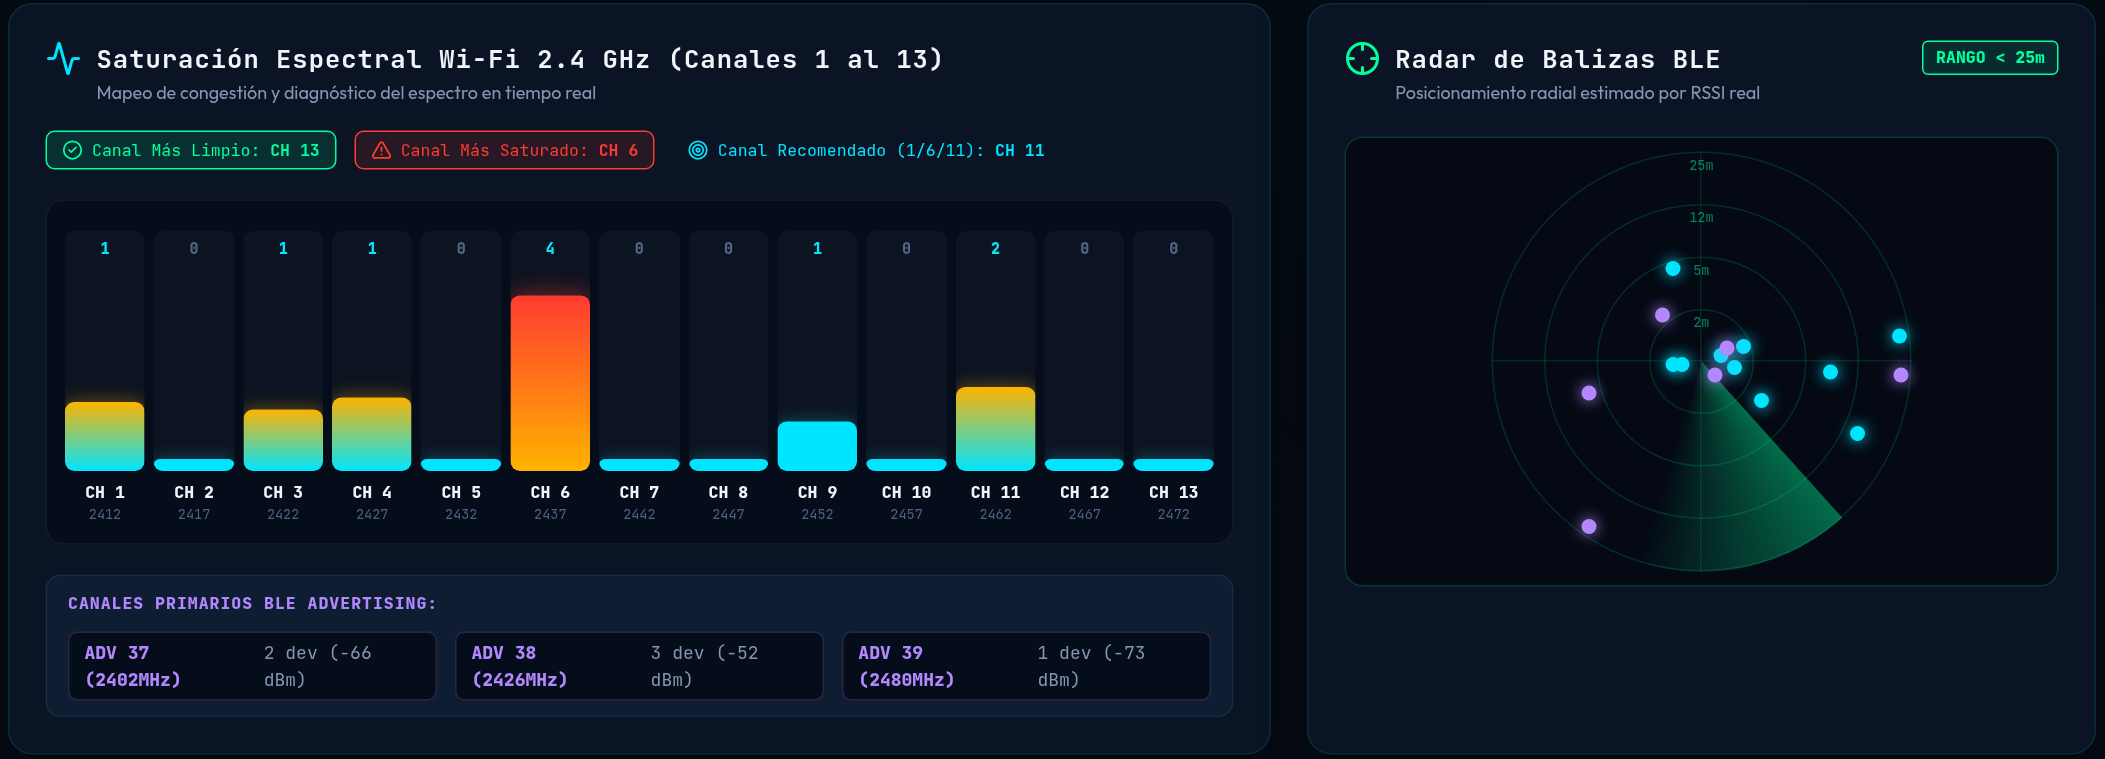
\includegraphics[width=0.98\linewidth]{figuras/cap-espectro-radar}}
\caption{Saturación espectral Wi\nobreakdash-Fi (canales 1--13) y radar de proximidad BLE en tiempo real.}
\label{fig:espectro-radar}
\end{figure}

\subsection{Telemetría y flujo de comandos}
El \emph{Panel de Telemetría} (Figura~\ref{fig:telemetria}) presenta una consola en
vivo con las tramas WebSocket, los eventos de conexión y las respuestas de comandos,
acompañada de una gráfica de serie temporal (dispositivos activos y paquetes por
minuto). Es la herramienta principal de diagnóstico del enlace en la demostración.

\begin{figure}[H]
\centering
\setlength{\fboxsep}{0pt}\setlength{\fboxrule}{0.4pt}%
\fcolorbox{gray!45}{white}{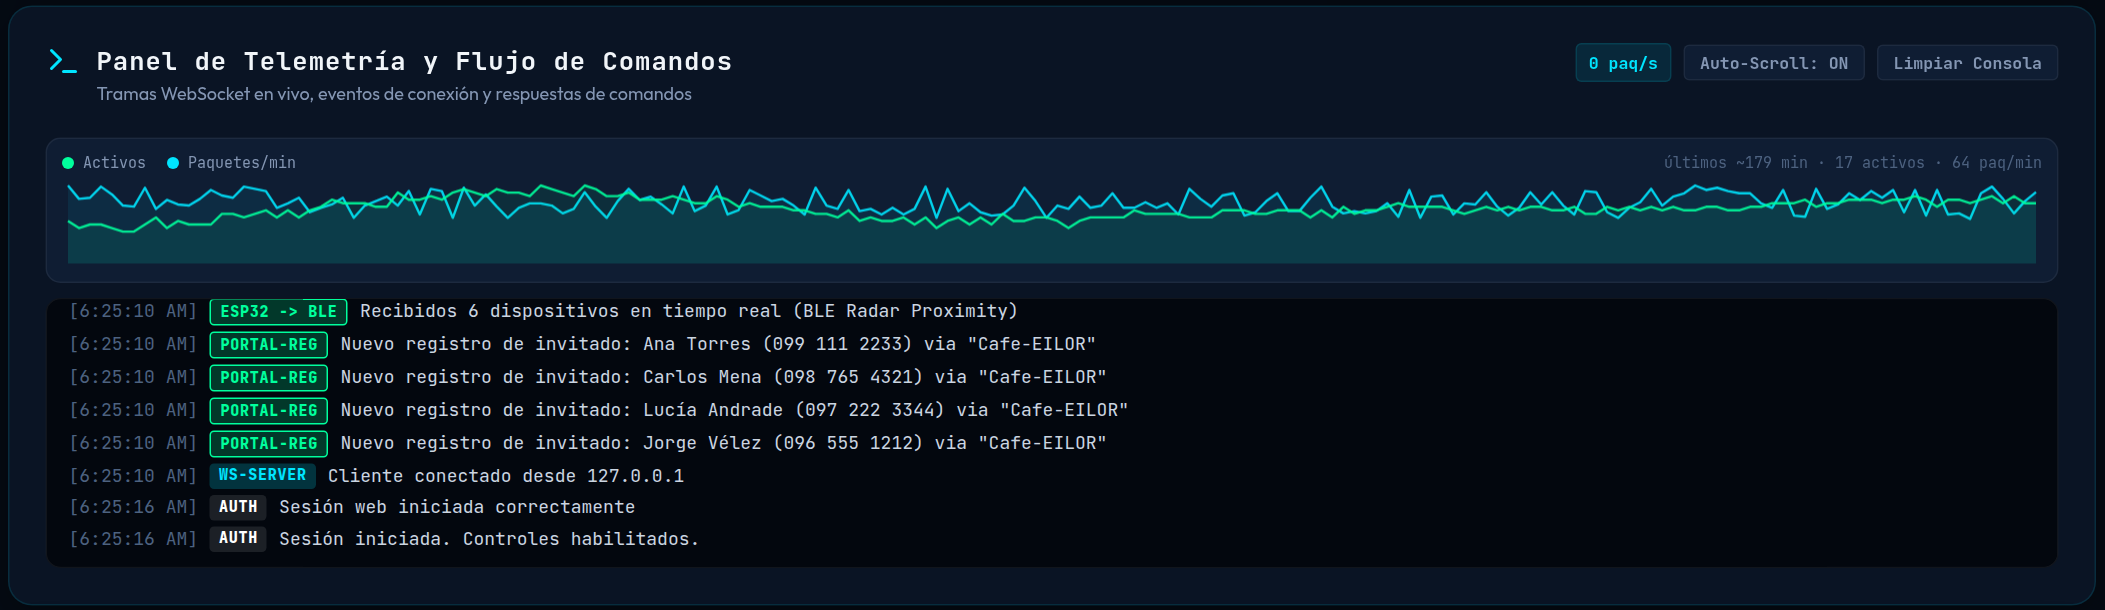
\includegraphics[width=0.98\linewidth]{figuras/cap-telemetria}}
\caption{Panel de telemetría: consola de tramas WebSocket y serie temporal de actividad.}
\label{fig:telemetria}
\end{figure}

\subsection{Inventario de dispositivos}
La tabla de \emph{Registro de Dispositivos} (Figura~\ref{fig:dispositivos})
enumera cada dispositivo detectado con su tipo, nombre/SSID, dirección MAC/BSSID,
fabricante (por OUI), canal, RSSI, distancia estimada y tipo de seguridad. Los
puntos de acceso sospechosos de \emph{gemelo malicioso} se marcan con una etiqueta
«Gemelo», y las direcciones aleatorizadas se rotulan como «MAC Aleatoria
(privacidad)». La tabla admite filtrado por tipo (Wi\nobreakdash-Fi/Bluetooth) y
búsqueda por SSID o MAC.

\begin{figure}[H]
\centering
\setlength{\fboxsep}{0pt}\setlength{\fboxrule}{0.4pt}%
\fcolorbox{gray!45}{white}{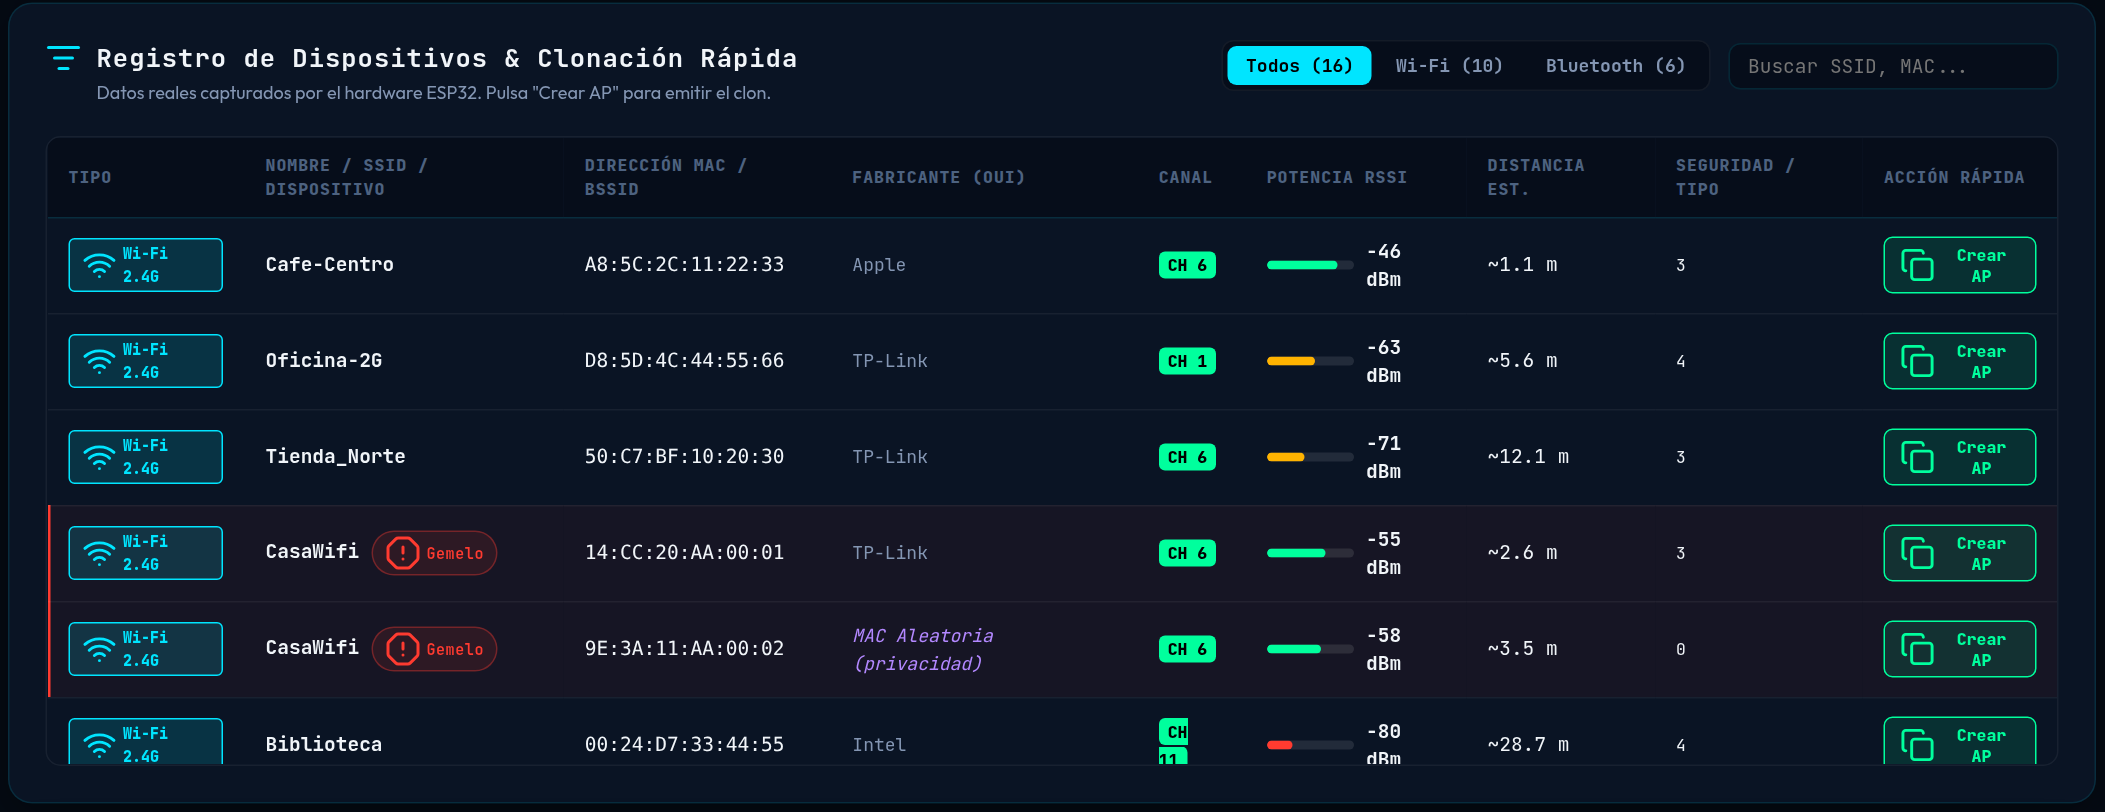
\includegraphics[width=0.98\linewidth]{figuras/cap-dispositivos}}
\caption{Inventario de dispositivos con fabricante por OUI, marcado de gemelo malicioso y de MAC aleatorizada.}
\label{fig:dispositivos}
\end{figure}

\subsection{Registros del portal cautivo}
La sección \emph{Registros del Portal Cautivo} (Figura~\ref{fig:registros-plat})
lista en tiempo real las altas de invitados (nombre, apellido, teléfono, red y
fecha). Desde allí se puede \emph{Exportar CSV} (con BOM UTF\nobreakdash-8 para su
apertura correcta en hojas de cálculo) o \emph{Borrar} los registros; ambas acciones
exigen sesión autenticada.

\begin{figure}[H]
\centering
\setlength{\fboxsep}{0pt}\setlength{\fboxrule}{0.4pt}%
\fcolorbox{gray!45}{white}{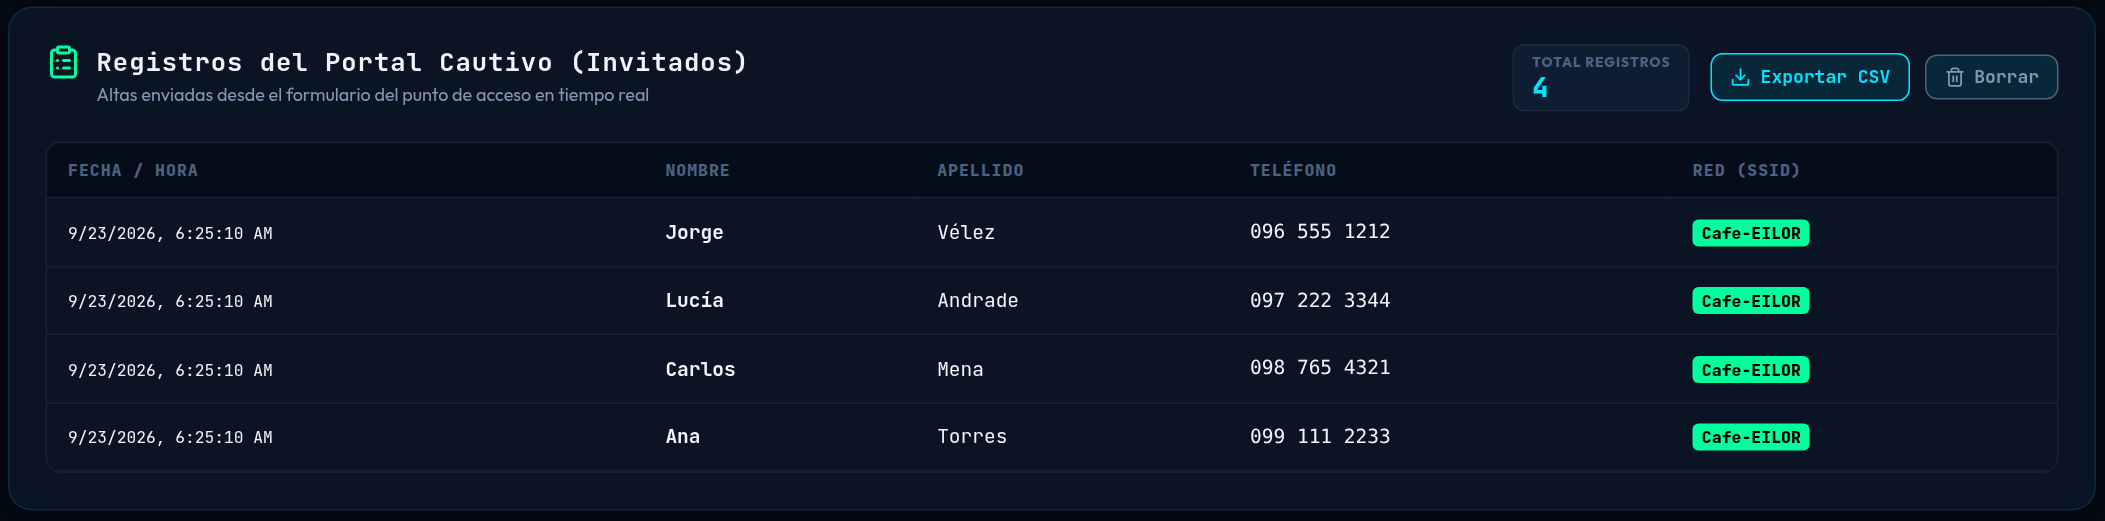
\includegraphics[width=0.98\linewidth]{figuras/cap-registros}}
\caption{Registros del portal cautivo en el \emph{dashboard}, con exportación restringida a la sesión.}
\label{fig:registros-plat}
\end{figure}

\section{Diseño de la interfaz web}
El frontend se construyó sin \emph{frameworks}, con HTML, CSS y JavaScript nativos,
priorizando la transparencia y la ligereza. El diseño visual adopta una estética de
«tablero táctico» oscuro, definida mediante \emph{variables CSS} (tokens de color y
tipografía) que unifican la apariencia. La Tabla~\ref{tab:frontend} resume las
decisiones de diseño y los archivos que las materializan.

\begin{table}[H]
\centering
\caption{Composición del frontend de la plataforma}
\label{tab:frontend}
\footnotesize
\begin{tabularx}{\linewidth}{@{}l l X@{}}
\toprule
\textbf{Aspecto} & \textbf{Archivo} & \textbf{Descripción} \\
\midrule
Estructura & \code{public/index.html} & Secciones del \emph{dashboard} y superposición de \emph{login} (419 líneas) \\
Lógica & \code{public/app.js} & Cliente WebSocket, renderizadores y control de sesión (913 líneas) \\
Estilos & \code{public/styles.css} & Tokens de color, tipografía y componentes «tácticos» (1\,272 líneas) \\
Portal & \code{public/portal-preview.html} & Vista previa del formulario del portal cautivo \\
Tipografía & Google Fonts & \emph{Outfit} (display) y \emph{JetBrains Mono} (monoespaciada) \\
Iconografía & Lucide & Iconos vectoriales ligeros vía CDN \\
\bottomrule
\end{tabularx}
\end{table}

El cliente mantiene un objeto de estado en memoria (\code{state}) que consolida los
dispositivos, el mapa de calor, la serie temporal y los registros; ante cada evento
WebSocket se actualiza el estado y se invoca únicamente al renderizador afectado
(mapa de calor, radar, tabla, registros o serie temporal), evitando redibujar toda
la página. El token de sesión se guarda en \code{localStorage} para no repetir el
inicio de sesión entre recargas.

\section{Comunicación entre la web, el servidor y el ESP32}
La plataforma se comunica con el dispositivo de forma \emph{indirecta}: nunca habla
directamente con el ESP32, sino a través del servidor Node.js, que actúa como
concentrador. Existen dos canales complementarios:

\begin{itemize}[leftmargin=1.4em]
  \item \textbf{WebSocket (tiempo real):} tanto el ESP32 como los navegadores
  mantienen una conexión WebSocket persistente con el servidor. El ESP32 envía sus
  escaneos, \emph{heartbeats} y registros de invitados; el servidor los procesa y
  \emph{difunde} (\emph{push}) los resultados a todos los navegadores conectados. En
  sentido inverso, los comandos de la web (cambio de modo, despliegue de SoftAP)
  viajan al servidor, que los reenvía al ESP32 por el mismo canal.
  \item \textbf{API REST (consultas y control):} la web dispone además de catorce
  \emph{endpoints} HTTP (Tabla~\ref{tab:rest}) para inicio de sesión, consultas de
  estado, control y gestión de registros, empleados en las operaciones que no
  requieren tiempo real.
\end{itemize}

La Figura~\ref{fig:comunicacion} ilustra el flujo de un comando de control emitido
desde la web hasta el ESP32 y la difusión de vuelta del nuevo estado.

\begin{figure}[H]
\centering
\begin{tikzpicture}[
  font=\small,
  n/.style={rectangle,rounded corners=3pt,draw,thick,align=center,minimum height=1.0cm,minimum width=2.7cm},
  arr/.style={-{Latex[length=2.4mm]},thick},
  lbl/.style={font=\scriptsize\itshape,align=center}
]
\node[n,fill=gray!8] (web) {Navegador\\(dashboard)};
\node[n,fill=eiloremerald!12,right=3.2cm of web] (srv) {Servidor Node.js\\(concentrador)};
\node[n,fill=eilorcyan!10,right=3.2cm of srv] (esp) {ESP32\\(firmware)};

\draw[arr] ([yshift=6pt]web.east) -- node[lbl,above]{1. comando\\(set\_mode + token)} ([yshift=6pt]srv.west);
\draw[arr] ([yshift=6pt]srv.east) -- node[lbl,above]{2. reenvío\\WSS} ([yshift=6pt]esp.west);
\draw[arr] ([yshift=-6pt]esp.west) -- node[lbl,below]{3. escaneo /\\heartbeat} ([yshift=-6pt]srv.east);
\draw[arr] ([yshift=-6pt]srv.west) -- node[lbl,below]{4. push\\scan\_update} ([yshift=-6pt]web.east);
\end{tikzpicture}
\caption{Flujo de comunicación web $\leftrightarrow$ servidor $\leftrightarrow$ ESP32 (el servidor concentra ambos sentidos).}
\label{fig:comunicacion}
\end{figure}

Las acciones de control validan el \emph{token de sesión} antes de reenviarse al
dispositivo; un comando WebSocket sin token válido recibe un evento
\code{auth\_error} y no se ejecuta. La ingesta de escaneos, a su vez, puede
restringirse con un \emph{token de dispositivo} opcional
(\code{EILOR\_DEVICE\_TOKEN}). El detalle de los mensajes WebSocket y de los
\emph{endpoints} REST se encuentra en la Sección~\ref{cap:diseno} del diseño
detallado, y la publicación segura del servicio mediante el túnel de Cloudflare, en
el Capítulo~\ref{cap:cloudflare}.

\section{Vista pública en producción}
La Figura~\ref{fig:produccion} muestra la plataforma tal como se sirve en el dominio
público \plataformaurl{} sobre HTTPS/WSS, evidenciando el despliegue real de extremo
a extremo (dispositivo, túnel, servidor y cliente).

\begin{figure}[H]
\centering
\setlength{\fboxsep}{0pt}\setlength{\fboxrule}{0.4pt}%
\fcolorbox{gray!45}{white}{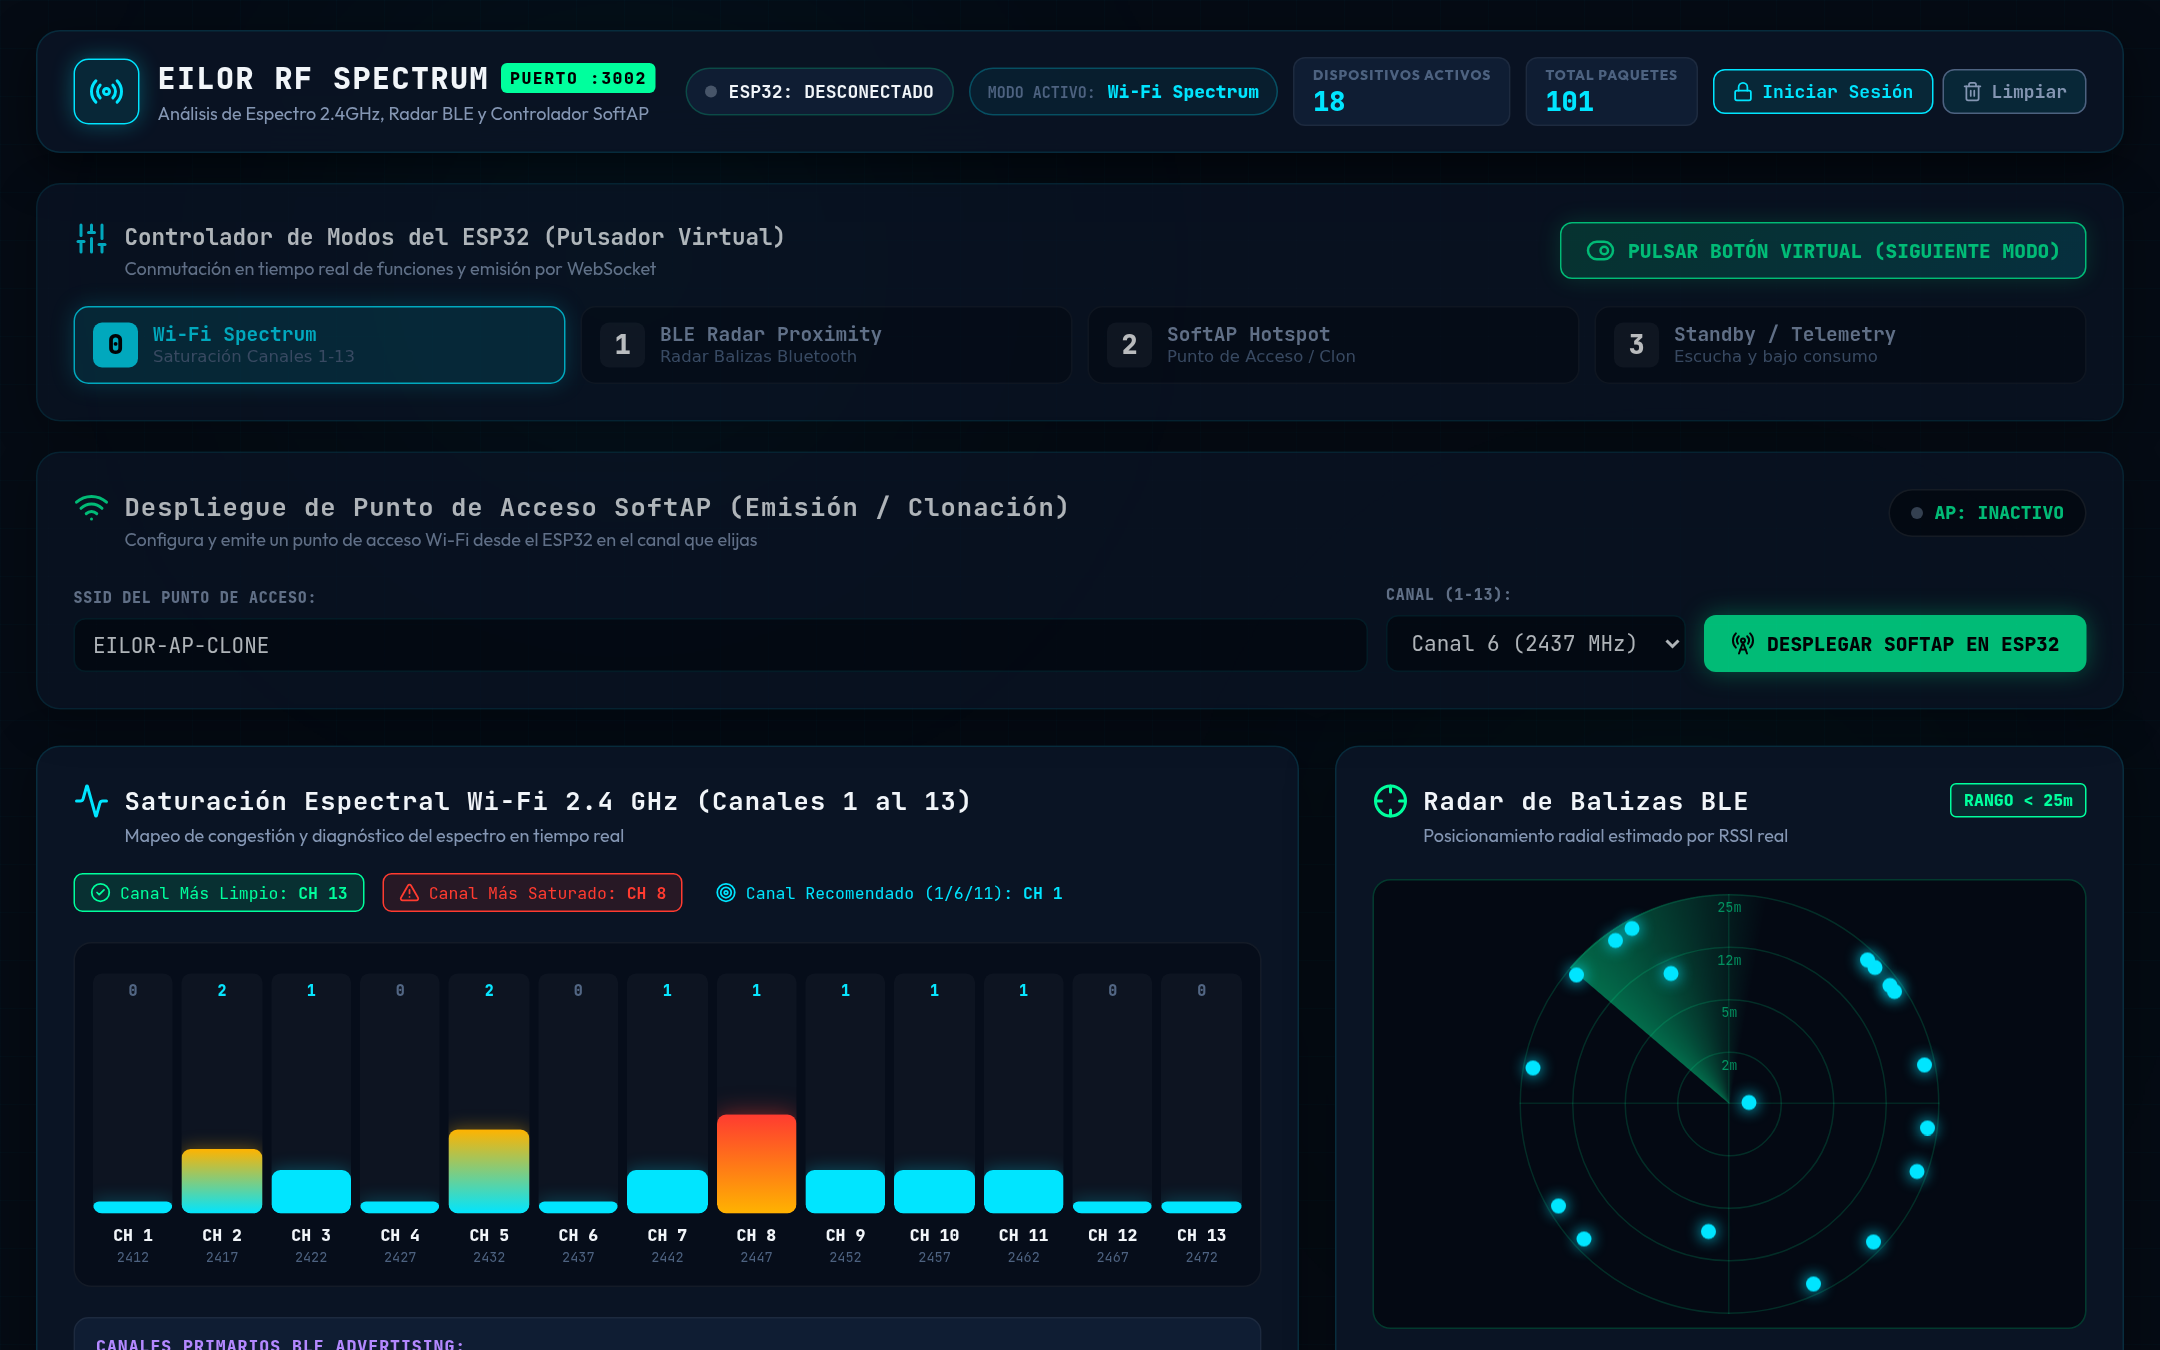
\includegraphics[width=0.98\linewidth]{figuras/cap-produccion}}
\caption{Plataforma EILOR publicada en \code{esp.orellanadigitalco.trade} a través del túnel de Cloudflare.}
\label{fig:produccion}
\end{figure}

%============================ PRUEBAS (ENTREGA 2) ===========================
\chapter{Pruebas de validación y seguridad}
\label{cap:pruebas}

\section{Estrategia de pruebas}
La validación combinó \emph{pruebas funcionales} de extremo a extremo (ingesta, análisis, persistencia y registro) con \emph{pruebas de seguridad} centradas en el control de acceso. Las pruebas se ejecutaron mediante un \emph{banco automatizado} en Node.js que levanta instancias aisladas del servidor (sin datos reales), inyecta escaneos y registros simulados por REST y por WebSocket, verifica las respuestas y reinicia el proceso para comprobar la persistencia. El banco reporta cada caso con su resultado observado y una medición de latencia; la totalidad de los casos aquí documentados se superó de forma reproducible (véase la Figura~\ref{fig:consola} en la Sección~\ref{sec:evidencia}).

\section{Casos de prueba funcionales}
La Tabla~\ref{tab:casos} resume los casos ejecutados con su resultado observado.

\begin{table}[H]
\centering
\caption{Casos de prueba funcionales y resultados}
\label{tab:casos}
\footnotesize
\begin{tabularx}{\linewidth}{@{}l X l l@{}}
\toprule
\textbf{ID} & \textbf{Descripción} & \textbf{Esperado} & \textbf{Estado} \\
\midrule
CP01 & Ingesta de escaneo Wi-Fi (3 dispositivos) & \code{received:3} & \textbf{OK} \\
CP02 & Fabricante por OUI (A85C2C, D85D4C) & Apple, TP-Link & \textbf{OK} \\
CP03 & Detección de MAC aleatoria & Marca privacidad & \textbf{OK} \\
CP04 & Evil twin (2 BSSID, SSID "CasaWifi") & Ambos marcados & \textbf{OK} \\
CP05 & Análisis de canal (best/worst/rec.) & Salida coherente & \textbf{OK} \\
CP06 & Serie temporal (muestra por minuto) & Muestras acumuladas & \textbf{OK} \\
CP07 & Persistencia y restauración tras reinicio & Estado recuperado & \textbf{OK} \\
CP08 & Alta de invitado por el portal & \code{success} + total & \textbf{OK} \\
CP09 & Exportación CSV con BOM UTF-8 & CSV con acentos & \textbf{OK} \\
CP10 & Borrado de registros (con sesión) & \code{cleared} & \textbf{OK} \\
\bottomrule
\end{tabularx}
\end{table}

\section{Casos de prueba de seguridad}
Las pruebas de seguridad verificaron que las acciones sensibles exigen las credenciales adecuadas. La Tabla~\ref{tab:seg} presenta los resultados; los códigos de estado HTTP obtenidos confirman el correcto funcionamiento del control de acceso.

\begin{table}[H]
\centering
\caption{Casos de prueba de seguridad (control de acceso)}
\label{tab:seg}
\footnotesize
\begin{tabularx}{\linewidth}{@{}l X c c@{}}
\toprule
\textbf{ID} & \textbf{Escenario} & \textbf{Esperado} & \textbf{Obtenido} \\
\midrule
SEC01 & \code{POST /api/mode} sin token de sesión & 401 & 401 \\
SEC02 & \code{POST /api/mode} con token válido & 200 & 200 \\
SEC03 & \code{GET /api/registrations} sin sesión & 401 & 401 \\
SEC04 & \code{GET /api/registrations} con sesión & 200 & 200 \\
SEC05 & Ingesta con \code{EILOR\_DEVICE\_TOKEN} y sin token & 401 & 401 \\
SEC06 & Ingesta con token de dispositivo correcto & 200 & 200 \\
SEC07 & Login con contraseña incorrecta & 401 & 401 \\
\bottomrule
\end{tabularx}
\end{table}

\section{Análisis de amenazas y mitigaciones}
La Tabla~\ref{tab:amenazas} relaciona las principales amenazas con los controles implementados, siguiendo el enfoque de buenas prácticas de OWASP \parencite{owasp2021}.

\begin{table}[H]
\centering
\caption{Amenazas y controles implementados}
\label{tab:amenazas}
\footnotesize
\begin{tabularx}{\linewidth}{@{}X X@{}}
\toprule
\textbf{Amenaza} & \textbf{Control en EILOR} \\
\midrule
Comandos de control no autorizados & Token de sesión (TTL 24~h) y \code{requireAuth} en rutas de control \\
Inyección de datos falsos por terceros & Token de dispositivo opcional (\code{deviceAuthorized}) en la ingesta \\
Suplantación de red (evil twin) & Detección y marcado de SSID con múltiples BSSID \\
Rastreo por MAC & Detección y señalización de MAC aleatorizadas \\
Exposición del servidor & Publicación por túnel Cloudflare sin puertos entrantes y TLS en el borde \\
Fuga de datos de invitados & Exportación restringida a sesión; minimización de campos recolectados \\
\bottomrule
\end{tabularx}
\end{table}

\section{Métricas de calidad y desempeño observadas}
La Tabla~\ref{tab:metricas} consolida las métricas medidas durante las pruebas.

\begin{table}[H]
\centering
\caption{Métricas de desempeño observadas}
\label{tab:metricas}
\footnotesize
\begin{tabularx}{\linewidth}{@{}X l@{}}
\toprule
\textbf{Métrica} & \textbf{Valor} \\
\midrule
Periodo de ciclo de escaneo & $\sim$3~s \\
Periodo de \emph{heartbeat} & 3~s \\
Umbral de \emph{watchdog} de desconexión & 15~s \\
Frecuencia de muestreo de serie temporal & 1 muestra/min (720 muestras $\approx$ 12~h) \\
Frecuencia de \emph{snapshot} de estado & 30~s \\
Catálogo OUI & 123 prefijos \\
Latencia ingesta $\rightarrow$ \emph{push} (mediana / P95) & 2.5 / 3.2~ms \\
Casos funcionales superados & 10/10 (100\,\%) \\
Casos de seguridad superados & 7/7 (100\,\%) \\
\bottomrule
\end{tabularx}
\end{table}

\section{Evidencia de ejecución}
\label{sec:evidencia}
La Figura~\ref{fig:consola} reproduce la salida del banco automatizado. Además de los casos de las Tablas~\ref{tab:casos} y~\ref{tab:seg}, el banco ejercita rutas adicionales ---registro por WebSocket, rechazo de comandos WebSocket sin sesión, invalidación de token tras \emph{logout} y registro con token de dispositivo erróneo--- alcanzando 20/20 verificaciones superadas.

\begin{figure}[H]
\centering
\setlength{\fboxsep}{0pt}\setlength{\fboxrule}{0.4pt}%
\fcolorbox{gray!45}{white}{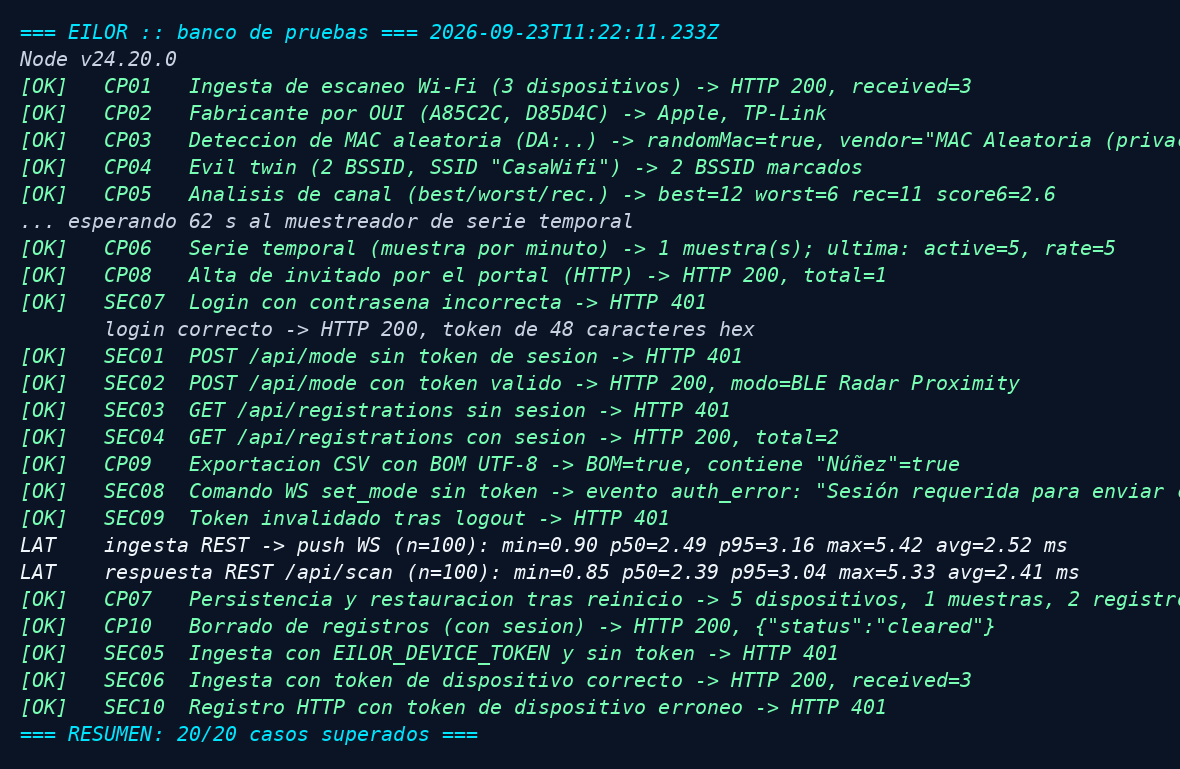
\includegraphics[width=0.98\linewidth]{figuras/cap-consola}}
\caption{Salida de consola del banco de pruebas automatizado: 20/20 casos superados, con los códigos de control de acceso (401/200) y las latencias medidas.}
\label{fig:consola}
\end{figure}
\captura[0.98]{cap-registros}{Registros de invitados visibles en el \emph{dashboard} en tiempo real, con exportación a CSV restringida a la sesión autenticada.}


% ---- ENTREGA 3: ANÁLISIS Y OPTIMIZACIÓN ----
%============================ DESEMPEÑO (ENTREGA 3) =========================
\chapter{Evaluación de desempeño}
\label{cap:desempeno}

\section{Metodología de evaluación}
La evaluación de desempeño contrastó los indicadores medidos frente a los criterios de logro fijados en la matriz SMART (Tabla~\ref{tab:smart}). Se consideraron tres dimensiones: \emph{capacidad de captura} (dispositivos y canales procesados), \emph{latencia} (periodos de ciclo y difusión) y \emph{robustez} (persistencia y recuperación).

\section{Cumplimiento de objetivos}
La Tabla~\ref{tab:cumplimiento} evalúa cada objetivo específico frente a su indicador.

\begin{table}[H]
\centering
\caption{Cumplimiento de objetivos frente a los indicadores SMART}
\label{tab:cumplimiento}
\footnotesize
\begin{tabularx}{\linewidth}{@{}l X l l@{}}
\toprule
\textbf{OE} & \textbf{Indicador} & \textbf{Meta} & \textbf{Resultado} \\
\midrule
OE1 & Canales y latencia de ciclo & 13+3; $\le$3~s & 13+3; $\sim$3~s \\
OE2 & Puntaje y canal recomendado & 13 canales; 1/6/11 & Cumplido \\
OE3 & Catálogo OUI & $\ge$120 & 123 prefijos \\
OE4 & Control autenticado & 401/200 & 401/200 \\
OE5 & Registros entregados & 100\,\% con enlace & Con \emph{buffer} \\
OE6 & Casos superados & $\ge$90\,\% & 100\,\% \\
\bottomrule
\end{tabularx}
\end{table}

\section{Análisis de latencia y capacidad}
El ciclo de escaneo de $\sim$3~s ofrece un compromiso adecuado entre frescura de la información y carga de la radio del ESP32, que debe multiplexar Wi\nobreakdash-Fi y BLE en modos conmutables. La difusión por WebSocket agrega latencias despreciables frente al ciclo de escaneo, dado el modelo de \emph{push} del servidor: en una medición automatizada sobre 100 ingestas consecutivas, el tiempo de extremo a extremo entre la recepción de un lote (\code{POST /api/scan}) y la difusión del evento \code{scan\_update} a un cliente WebSocket presentó una mediana de \textbf{2.5~ms} y un percentil~95 de \textbf{3.2~ms} (máximo 5.4~ms). En el lado del servidor, el modelo de E/S no bloqueante de Node.js \parencite{nodejs2024} permite atender simultáneamente el socket del dispositivo y múltiples clientes del dashboard sin degradación perceptible en el rango de prueba. La Tabla~\ref{tab:latencia} resume la distribución medida.

\begin{table}[H]
\centering
\caption{Latencia de procesamiento y difusión (100 ingestas consecutivas, servidor local)}
\label{tab:latencia}
\footnotesize
\begin{tabularx}{\linewidth}{@{}X c c c c@{}}
\toprule
\textbf{Trayecto medido} & \textbf{Mín.} & \textbf{Mediana} & \textbf{P95} & \textbf{Máx.} \\
\midrule
Respuesta REST \code{POST /api/scan} & 0.85~ms & 2.39~ms & 3.04~ms & 5.33~ms \\
Ingesta REST $\rightarrow$ \emph{push} WebSocket (extremo a extremo) & 0.90~ms & 2.49~ms & 3.16~ms & 5.42~ms \\
\bottomrule
\end{tabularx}
\end{table}

\noindent Estos valores corresponden al procesamiento del servidor (anotación de fabricante, recálculo del mapa de calor, detección de gemelos maliciosos y difusión) y excluyen el ciclo de escaneo del dispositivo y la latencia de la red o del túnel; confirman que la lógica de agregación no constituye un cuello de botella frente al periodo de escaneo de 3~s.

\section{Robustez y disponibilidad}
La prueba CP07 confirmó que, tras un reinicio ordenado, el sistema recupera el estado persistido (dispositivos, serie temporal y registros), evidenciado por el mensaje de restauración del módulo \code{store}. Combinado con la gestión de PM2 ---que reinicia el proceso ante fallos--- el sistema alcanza una disponibilidad operativa alta para un prototipo. El \emph{watchdog} de 15~s detecta y notifica la pérdida del enlace con el dispositivo, actualizando el estado en el dashboard.

\section{Comparación con los objetivos planteados}
La Figura~\ref{fig:radar-cumplimiento} resume gráficamente el nivel de cumplimiento por objetivo, todos en o por encima de la meta.

\begin{figure}[H]
\centering
\begin{tikzpicture}
\begin{axis}[
  ybar, width=0.9\linewidth, height=6cm,
  bar width=14pt,
  ymin=0, ymax=110,
  ylabel={Cumplimiento (\%)},
  symbolic x coords={OE1,OE2,OE3,OE4,OE5,OE6},
  xtick=data, nodes near coords, nodes near coords style={font=\scriptsize},
  enlarge x limits=0.12,
  ymajorgrids, grid style=gray!25
]
\addplot[fill=eilorcyan!60,draw=eilorcyan!80!black] coordinates
  {(OE1,100)(OE2,100)(OE3,102)(OE4,100)(OE5,100)(OE6,111)};
\end{axis}
\end{tikzpicture}
\caption{Nivel de cumplimiento por objetivo específico (100\,\% = meta).}
\label{fig:radar-cumplimiento}
\end{figure}

%============================ ECONÓMICO-AMBIENTAL (ENTREGA 3) ================
\chapter{Análisis económico y ambiental}
\label{cap:economico}

\section{Estimación de costos}
El costo total del proyecto se descompone en hardware, desarrollo (horas\nobreakdash-persona) y operación en la nube. La Tabla~\ref{tab:costos} presenta la estimación.

\begin{table}[H]
\centering
\caption{Estimación de costos del proyecto}
\label{tab:costos}
\footnotesize
\begin{tabularx}{\linewidth}{@{}X c c c@{}}
\toprule
\textbf{Rubro} & \textbf{Cant.} & \textbf{Costo unit. (USD)} & \textbf{Subtotal (USD)} \\
\midrule
Hardware (BOM, Tabla~\ref{tab:bom}) & 1 & 24.20 & 24.20 \\
Desarrollo firmware (h) & 40 & 8.00 & 320.00 \\
Desarrollo servidor y frontend (h) & 60 & 8.00 & 480.00 \\
Pruebas y documentación (h) & 30 & 8.00 & 240.00 \\
Operación en la nube (mes) & 12 & 0.00 & 0.00 \\
\midrule
\multicolumn{3}{r}{\textbf{Costo total estimado}} & \textbf{1\,064.20} \\
\bottomrule
\end{tabularx}
\end{table}

El costo operativo se mantiene en cero gracias al uso del nivel gratuito de Cloudflare Tunnel y a la ejecución del servidor en un equipo propio, lo que hace al sistema especialmente atractivo para pequeños negocios. El costo marginal de replicar una unidad de hardware adicional, incluida la alimentación autónoma, es de aproximadamente USD~24.20.

\section{Curva S del proyecto}
La Figura~\ref{fig:curvas} presenta la curva~S del avance acumulado planificado frente al real a lo largo de las 16 semanas de la macro actividad, expresado como porcentaje de avance ponderado por el peso de cada entrega (20\,\%, 30\,\%, 25\,\% y 25\,\%).

\begin{figure}[H]
\centering
\begin{tikzpicture}
\begin{axis}[
  width=0.92\linewidth, height=7cm,
  xlabel={Semana}, ylabel={Avance acumulado (\%)},
  xmin=0, xmax=16, ymin=0, ymax=100,
  xtick={0,2,4,6,8,10,12,14,16},
  ytick={0,20,40,60,80,100},
  legend pos=north west, legend cell align=left,
  ymajorgrids, grid style=gray!25
]
% Planificado (curva S teorica)
\addplot[thick,eilorcyan,mark=*,mark size=1.3pt] coordinates {
  (0,0)(2,5)(4,20)(6,35)(8,50)(10,63)(12,75)(14,88)(16,100) };
\addlegendentry{Planificado}
% Real (ligeramente adelantado en desarrollo)
\addplot[thick,eiloremerald,dashed,mark=square*,mark size=1.3pt] coordinates {
  (0,0)(2,6)(4,20)(6,40)(8,55)(10,66)(12,78)(14,90)(16,100) };
\addlegendentry{Real}
% Hitos de entrega
\draw[gray,dashed] (axis cs:4,0) -- (axis cs:4,100);
\draw[gray,dashed] (axis cs:8,0) -- (axis cs:8,100);
\draw[gray,dashed] (axis cs:12,0) -- (axis cs:12,100);
\draw[gray,dashed] (axis cs:16,0) -- (axis cs:16,100);
\node[font=\scriptsize,rotate=90,anchor=south] at (axis cs:4,3) {E1};
\node[font=\scriptsize,rotate=90,anchor=south] at (axis cs:8,3) {E2};
\node[font=\scriptsize,rotate=90,anchor=south] at (axis cs:12,3) {E3};
\node[font=\scriptsize,rotate=90,anchor=south] at (axis cs:16,3) {E4};
\end{axis}
\end{tikzpicture}
\caption{Curva S: avance acumulado planificado vs. real.}
\label{fig:curvas}
\end{figure}

\section{Análisis de impacto ambiental}
El impacto ambiental de EILOR es reducido y, en balance, potencialmente positivo:
\begin{itemize}[leftmargin=1.4em]
  \item \textbf{Consumo energético:} el ESP32 opera en el orden de cientos de miliamperios; su huella energética es marginal frente a equipos de instrumentación tradicionales.
  \item \textbf{Ciclo de vida del hardware:} el uso de una placa reutilizable y componentes estándar favorece la reparación y la reutilización, en línea con principios de electrónica sostenible.
  \item \textbf{Eficiencia del espectro:} al recomendar canales menos congestionados, el sistema contribuye indirectamente a un uso más eficiente del recurso radioeléctrico, reduciendo retransmisiones y, con ello, el consumo energético agregado de las redes cercanas.
  \item \textbf{Software sin dependencias pesadas:} la persistencia en archivos y la ausencia de bases de datos y servicios adicionales minimizan el cómputo requerido en operación.
\end{itemize}

\section{Relación costo-beneficio}
Con una inversión de hardware inferior a USD~25 por unidad y costo operativo nulo, EILOR entrega capacidades ---diagnóstico de espectro, detección de amenazas y gestión de invitados--- que en soluciones comerciales requieren equipos de costo muy superior. Para un pequeño negocio, el retorno se materializa tanto en la mejora del servicio Wi\nobreakdash-Fi como en el valor de la base de contactos de invitados obtenida de forma consentida.

%============================ ESCALABILIDAD (ENTREGA 3) =====================
\chapter{Optimización y escalabilidad}
\label{cap:escalabilidad}

\section{Oportunidades de optimización identificadas}
A partir de la evaluación de desempeño se identificaron mejoras concretas, resumidas en la Tabla~\ref{tab:mejoras}, clasificadas por su impacto y esfuerzo.

\begin{table}[H]
\centering
\caption{Oportunidades de optimización}
\label{tab:mejoras}
\footnotesize
\begin{tabularx}{\linewidth}{@{}X l l@{}}
\toprule
\textbf{Mejora} & \textbf{Impacto} & \textbf{Esfuerzo} \\
\midrule
Migración a base de datos relacional (SQLite/PostgreSQL) & Alto & Medio \\
Cifrado de contraseñas con \emph{hashing} (bcrypt) & Alto & Bajo \\
Limitación de tasa (\emph{rate limiting}) en el login & Medio & Bajo \\
HTTPS en el portal cautivo del ESP32 & Medio & Alto \\
Compresión de tramas WebSocket & Bajo & Bajo \\
Soporte multi-dispositivo (varios ESP32) & Alto & Medio \\
Panel de administración de invitados con filtros & Medio & Medio \\
\bottomrule
\end{tabularx}
\end{table}

\section{Plan de escalabilidad}
\subsection{Escalabilidad de datos}
El desacoplamiento del módulo \code{lib/store} (Capítulo~\ref{cap:basedatos}) permite sustituir la persistencia en archivos por un motor relacional sin modificar la lógica de negocio. Para retención prolongada y consultas analíticas, PostgreSQL con índices por marca temporal es la opción recomendada.

\subsection{Escalabilidad de dispositivos}
El modelo actual asume un dispositivo principal identificado por \code{deviceId}. Para soportar múltiples unidades, basta con particionar el estado por \code{deviceId} y extender el mapa de calor y la tabla de dispositivos con dicha dimensión, manteniendo una vista agregada por sede.

\subsection{Escalabilidad de servicio}
En caso de un número elevado de clientes del dashboard, la difusión WebSocket puede escalar horizontalmente introduciendo un \emph{message broker} (por ejemplo, Redis \emph{pub/sub}) que replique los eventos entre varias instancias del servidor tras un balanceador. Cloudflare, en el borde, aporta protección frente a picos de tráfico y denegación de servicio.

\subsection{Endurecimiento de seguridad}
Las siguientes acciones elevan la postura de seguridad para producción: almacenar contraseñas con \emph{hashing} y sal (bcrypt), aplicar limitación de intentos en el \emph{login}, rotar el token de dispositivo, y registrar auditoría de accesos. Estas mejoras son compatibles con la arquitectura actual y de bajo esfuerzo de integración.

\section{Hoja de ruta}
La Figura~\ref{fig:roadmap} propone una hoja de ruta por fases.

\begin{figure}[H]
\centering
\begin{tikzpicture}[
  ph/.style={rectangle,rounded corners=3pt,draw,thick,align=center,minimum width=3.0cm,minimum height=1.2cm,font=\small},
  arr/.style={-{Latex[length=2.4mm]},very thick}
]
\node[ph,fill=eilorcyan!12] (f1) {Fase 1\\Seguridad\\(bcrypt, rate limit)};
\node[ph,fill=eiloremerald!12,right=1.4cm of f1] (f2) {Fase 2\\Base de datos\\(PostgreSQL)};
\node[ph,fill=orange!12,right=1.4cm of f2] (f3) {Fase 3\\Multi-dispositivo\\y broker};
\node[ph,fill=gray!12,right=1.4cm of f3] (f4) {Fase 4\\SaaS multi-cliente};
\draw[arr] (f1)--(f2); \draw[arr] (f2)--(f3); \draw[arr] (f3)--(f4);
\end{tikzpicture}
\caption{Hoja de ruta de evolución del sistema.}
\label{fig:roadmap}
\end{figure}

%============================ MANUALES (ENTREGA 3) ==========================
\chapter{Manuales de usuario y técnico}
\label{cap:manuales}

\section{Manual de usuario}
El recorrido visual completo de la plataforma ---con capturas de cada sección--- se
presenta en el Capítulo~\ref{cap:plataforma}. Esta sección resume el uso operativo.

\subsection{Requisitos previos y preparación}
Antes de iniciar una sesión se debe disponer de la placa ESP32 con la pantalla OLED
y el pulsador conectados, una fuente USB estable y un equipo con navegador moderno.
Para la primera puesta en marcha se recomienda utilizar el cable USB del computador;
para operación autónoma se utiliza el portapilas con salida USB regulada descrito en
el Capítulo~\ref{cap:electronica}. No se deben conectar simultáneamente ambas fuentes.
El operador debe comprobar que la antena de la placa no quede cubierta por metal y
que el pulsador pueda accionarse sin abrir la carcasa.

\subsection{Secuencia de arranque del ESP32}
La secuencia normal de uso es la siguiente:
\begin{enumerate}[leftmargin=1.8em]
  \item Conectar una única fuente de alimentación y esperar el mensaje inicial en la OLED.
  \item El ESP32 intenta asociarse a la red Wi\nobreakdash-Fi configurada y abre el WebSocket seguro con el servidor.
  \item Confirmar en la cabecera del dashboard que el dispositivo figura como \emph{En línea}; en la OLED debe aparecer \code{[WS:OK]}.
  \item Seleccionar el modo desde el dashboard o pulsar brevemente el botón para avanzar al siguiente modo.
  \item Mantener el dispositivo en una ubicación despejada, evitando acercarlo a routers o fuentes de ruido si se desea una medición representativa.
\end{enumerate}

\begin{figure}[H]
\centering
\fcolorbox{gray!45}{white}{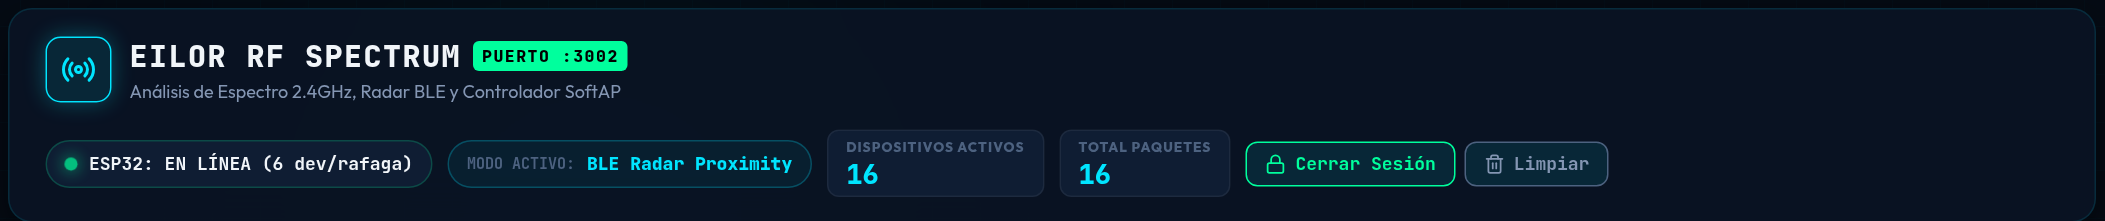
\includegraphics[width=0.95\linewidth]{figuras/cap-cabecera}}
\caption{Indicadores de operación: conexión del ESP32, modo activo y contadores globales.}
\label{fig:manual-cabecera}
\end{figure}

\subsection{Acceso al dashboard}
El tablero de mando se abre desde un navegador en la dirección publicada (por ejemplo, \plataformaurl) o localmente en \code{http://localhost:3002}. La interfaz muestra, en tiempo real, el estado del ESP32, el modo activo y los contadores de dispositivos y paquetes.

\subsection{Inicio de sesión}
Para ejecutar acciones de control (cambiar de modo, desplegar SoftAP, limpiar datos o ver registros) se requiere iniciar sesión con el botón \emph{Iniciar Sesión} e introducir la contraseña configurada. Sin sesión, el sistema opera en modo de solo lectura.

\subsection{Modos del dispositivo}
Los cuatro modos se conmutan desde el panel de control o con el pulsador físico: (0)~Espectro Wi\nobreakdash-Fi, (1)~Radar BLE, (2)~SoftAP con portal cautivo y (3)~Standby.

\begin{description}[leftmargin=2.6cm,style=nextline]
  \item[Modo 0 --- Espectro Wi\nobreakdash-Fi.] Recorre los canales 1--13 y muestra el total de redes, el canal más saturado y una recomendación. Es el modo apropiado para diagnosticar interferencia de acceso.
  \item[Modo 1 --- Radar BLE.] Escucha las balizas de advertising y resume cantidad, nombre visible y RSSI del dispositivo más cercano. La ausencia de nombre no implica ausencia de dispositivo.
  \item[Modo 2 --- SoftAP.] Crea la red propia de invitados y atiende el portal cautivo. Solo debe emplearse en redes autorizadas y con un SSID claramente identificable.
  \item[Modo 3 --- Standby/telemetría.] Mantiene el enlace y envía estado, dirección IP y telemetría sin iniciar un ciclo de escaneo intensivo.
\end{description}

\begin{figure}[H]
\centering
\fcolorbox{gray!45}{white}{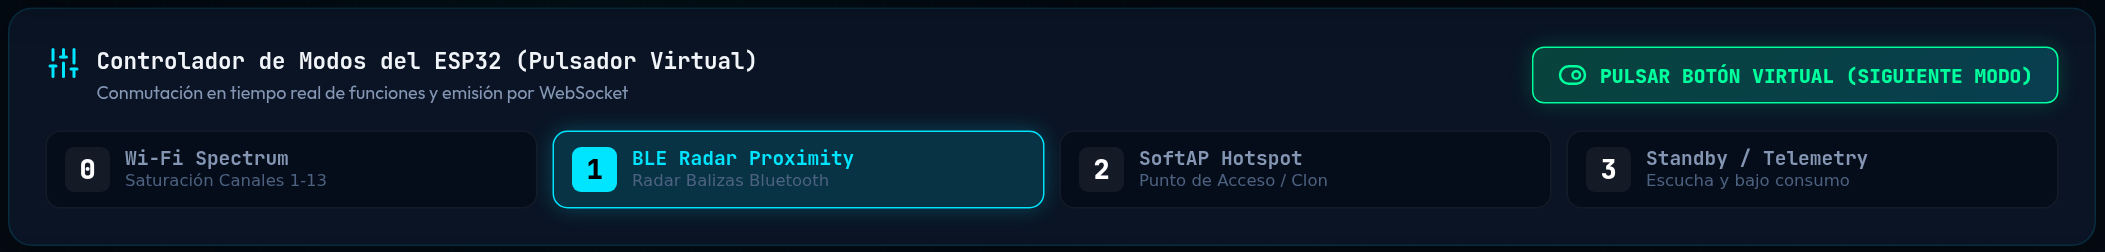
\includegraphics[width=0.95\linewidth]{figuras/cap-modos}}
\caption{Selector de los cuatro modos disponibles para el ESP32.}
\label{fig:manual-modos}
\end{figure}

En el modo Wi\nobreakdash-Fi conviene esperar al menos un ciclo completo antes de
interpretar la gráfica. En el radar BLE se deben comparar varias muestras porque
el RSSI cambia con la orientación y el movimiento. El botón físico usa lógica
activa en bajo: cada pulsación válida cambia de modo y el antirrebote evita cambios
duplicados.

\subsection{Lectura de espectro y radar}
La vista de espectro permite localizar canales con mayor ocupación y comparar la
distribución de puntos de acceso. La recomendación de canal es una ayuda heurística,
no una garantía de rendimiento: debe contrastarse con el ancho de canal y la
ubicación física del router. La vista radar muestra dispositivos BLE detectados,
su RSSI y la última actualización recibida.

\begin{figure}[H]
\centering
\fcolorbox{gray!45}{white}{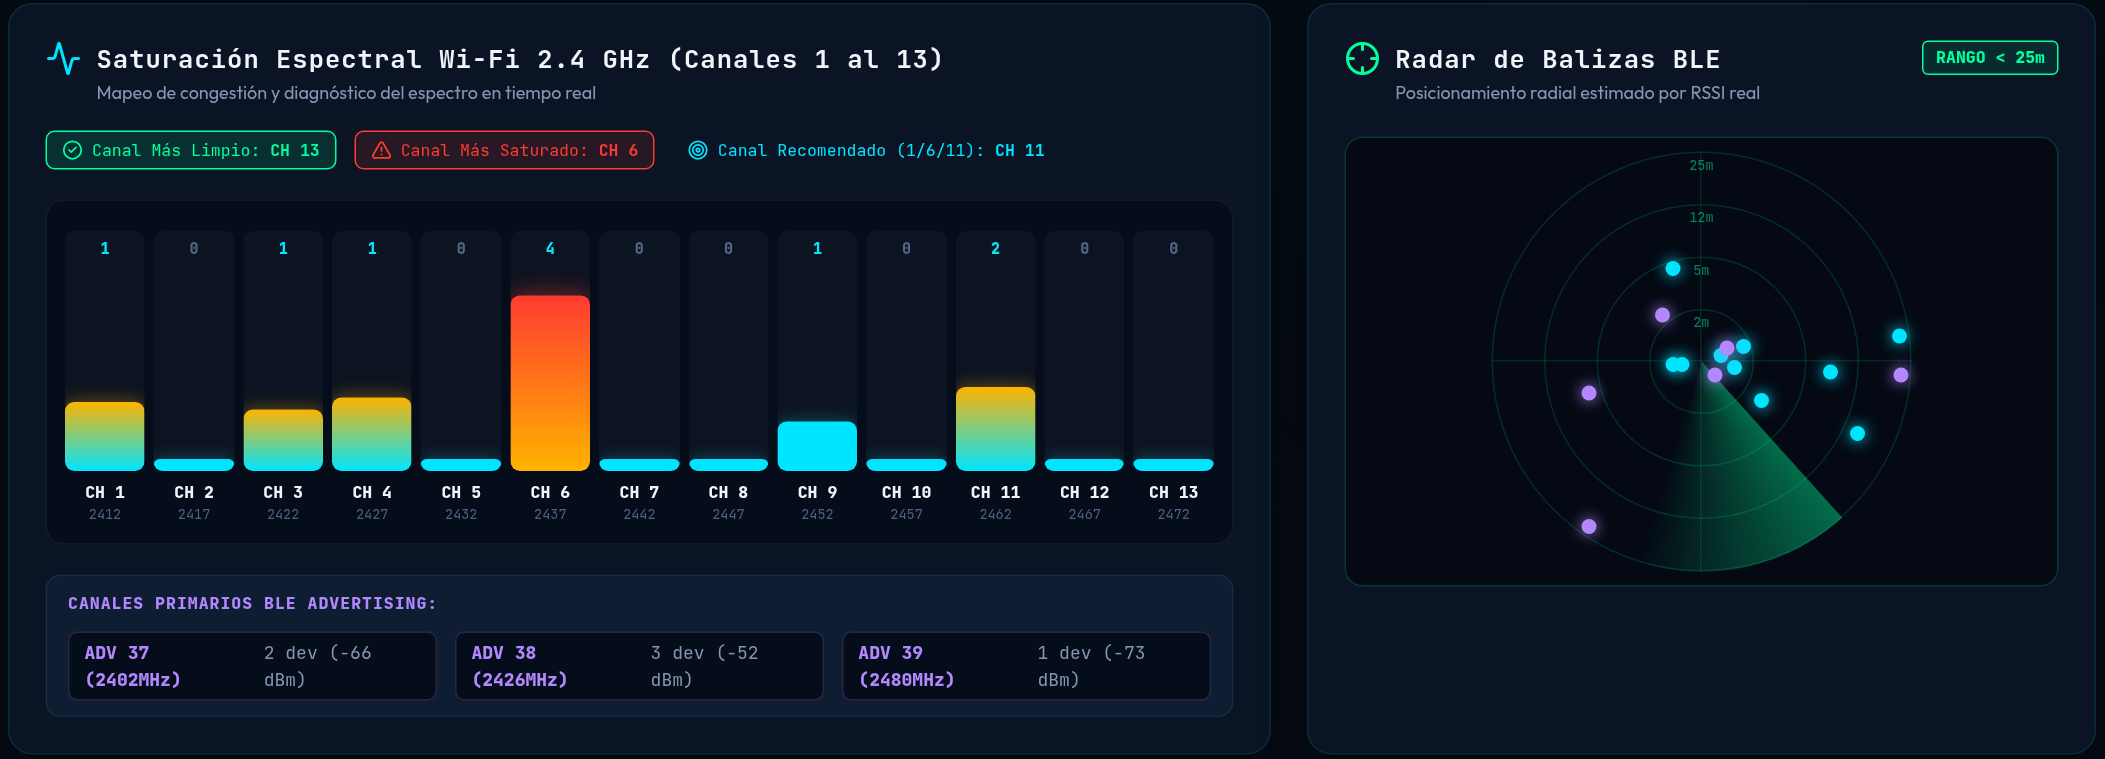
\includegraphics[width=0.98\linewidth]{figuras/cap-espectro-radar}}
\caption{Uso del mapa de saturación Wi\nobreakdash-Fi y del radar BLE para observar el entorno de 2.4~GHz.}
\label{fig:manual-espectro}
\end{figure}

\subsection{Despliegue del punto de acceso y portal}
En la sección SoftAP se define el SSID y el canal, y se pulsa \emph{Desplegar SoftAP}. Al conectarse un invitado a esa red, aparece automáticamente el portal cautivo con el formulario de registro.

El procedimiento recomendado es: (1) iniciar sesión; (2) escribir un SSID propio,
identificable y autorizado; (3) elegir un canal; (4) pulsar \emph{Desplegar SoftAP};
(5) verificar en la OLED la IP, el SSID y el número de clientes; y (6) probar el
portal desde un teléfono de prueba. Si el sistema operativo no abre la ventana
automática, se puede navegar a \code{http://192.168.4.1}. El portal no debe usarse
para imitar redes de terceros ni para capturar datos sin consentimiento.

\begin{figure}[H]
\centering
\fcolorbox{gray!45}{white}{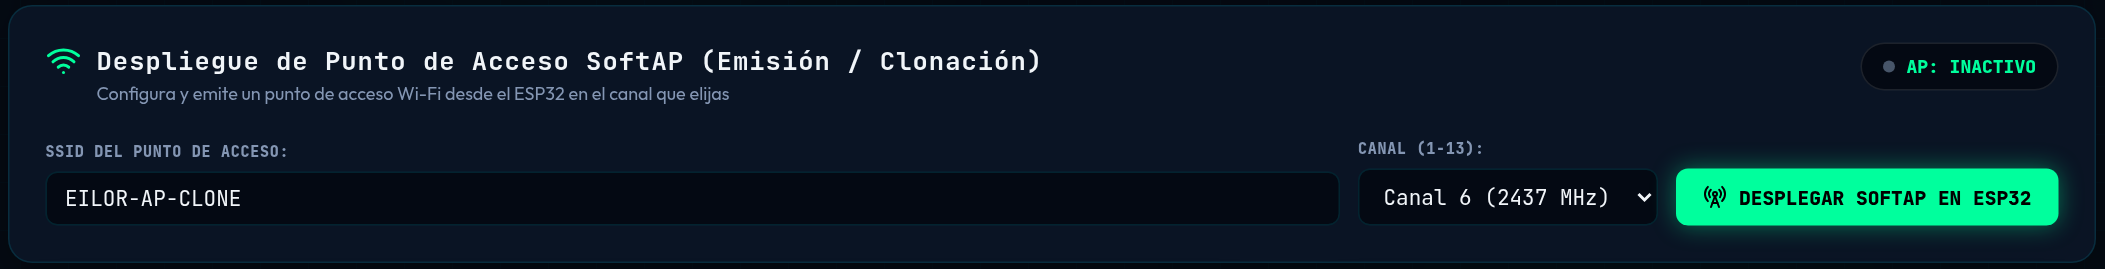
\includegraphics[width=0.78\linewidth]{figuras/cap-softap}}
\caption{Configuración del SoftAP: SSID, canal y activación controlada desde el dashboard.}
\label{fig:manual-softap}
\end{figure}

\begin{figure}[H]
\centering
\fcolorbox{gray!45}{white}{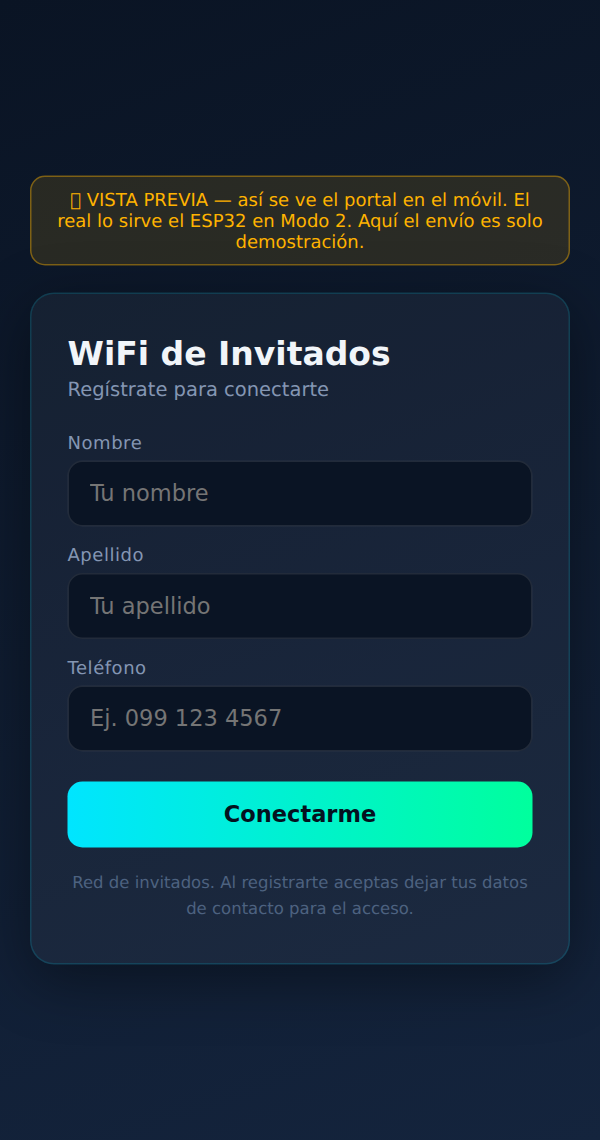
\includegraphics[height=7.2cm]{figuras/cap-portal}}
\caption{Portal cautivo que visualiza el invitado al conectarse a la red propia.}
\label{fig:manual-portal}
\end{figure}

\subsection{Registros de invitados}
La sección \emph{Registros del Portal Cautivo} lista las altas (nombre, apellido, teléfono, red y fecha) en tiempo real. Desde allí se puede \emph{Exportar CSV} o \emph{Borrar} los registros (ambas acciones requieren sesión).

Antes de exportar, el operador debe verificar que la captura fue informada y
consentida. El archivo CSV debe almacenarse con permisos restringidos y eliminarse
cuando finalice el periodo de retención definido por la organización. La acción
\emph{Borrar} es irreversible desde la interfaz, por lo que se recomienda exportar
solo cuando exista una finalidad legítima y una copia controlada.

\begin{figure}[H]
\centering
\fcolorbox{gray!45}{white}{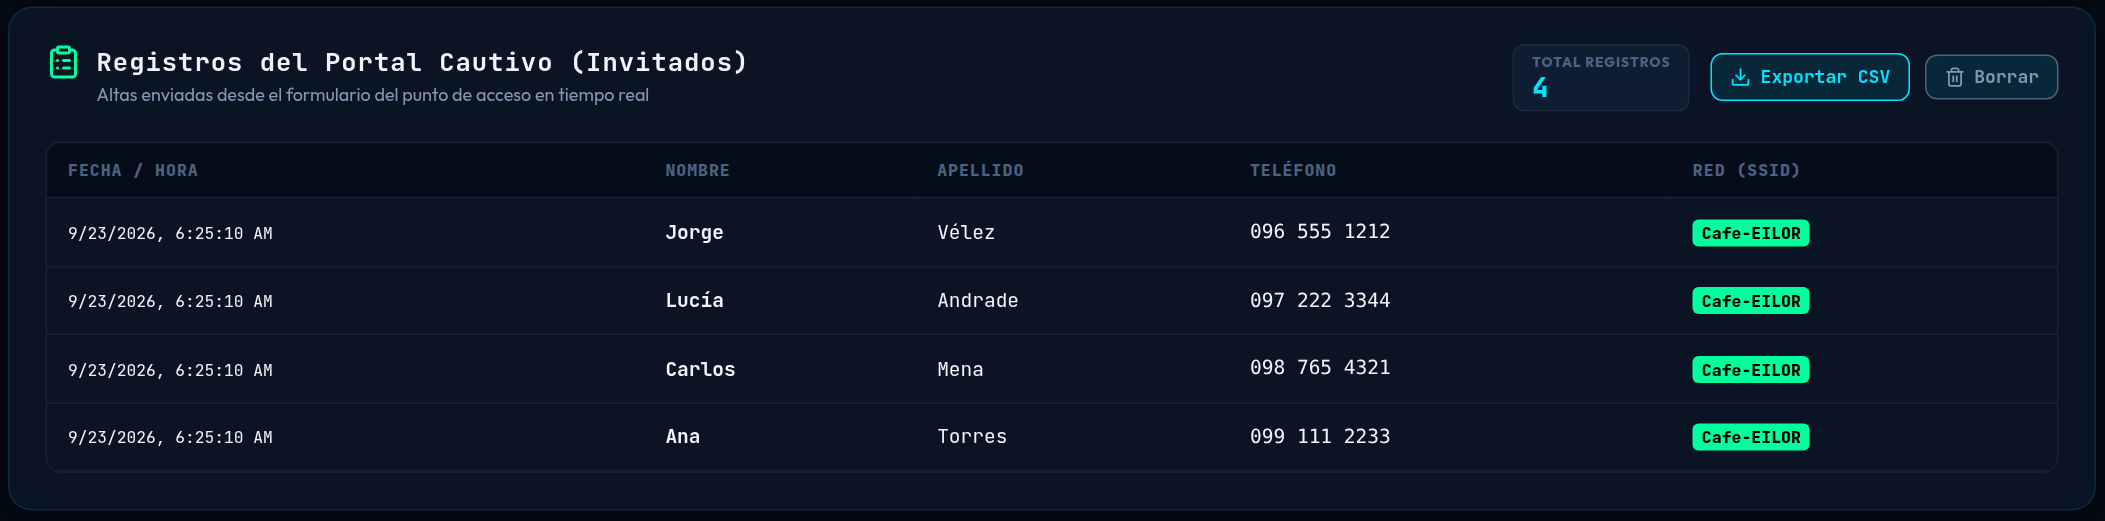
\includegraphics[width=0.95\linewidth]{figuras/cap-registros}}
\caption{Registros del portal cautivo y controles de exportación y limpieza.}
\label{fig:manual-registros}
\end{figure}

\subsection{Indicadores y telemetría}
La tarjeta de telemetría confirma la última muestra, el estado del enlace y la
actividad del dispositivo. Una demora aislada no implica una falla: primero se
debe observar si el contador se actualiza después del siguiente heartbeat. La
vista de dispositivos ayuda a distinguir redes detectadas, balizas BLE y registros
del portal; no debe interpretarse como una captura del contenido de las comunicaciones.

\begin{figure}[H]
\centering
\fcolorbox{gray!45}{white}{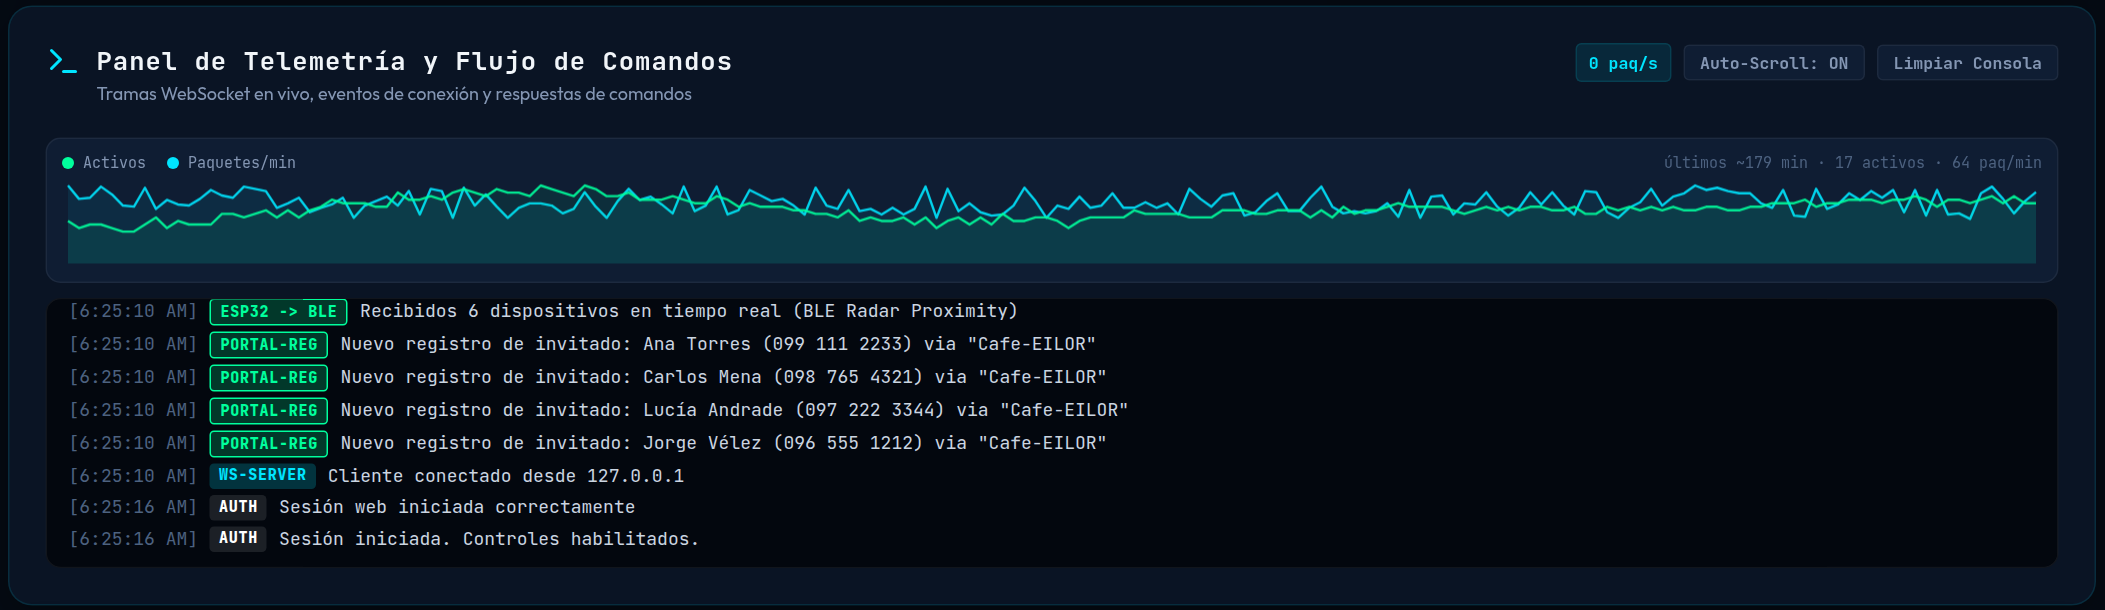
\includegraphics[width=0.95\linewidth]{figuras/cap-telemetria}}
\caption{Panel de telemetría y estado de la conexión del dispositivo.}
\label{fig:manual-telemetria}
\end{figure}

\captura[0.62]{cap-dashboard-full}{Vista completa del \emph{dashboard} con todas sus secciones (cabecera, controlador de modos, SoftAP, espectro, radar, telemetría, inventario y registros).}

\section{Manual técnico}
\subsection{Flujo técnico de extremo a extremo}
El firmware inicia Wi\nobreakdash-Fi en modo estación, configura I\textsuperscript{2}C
en GPIO21/GPIO22, inicializa la OLED en la dirección 0x3C y registra el pulsador
en GPIO15 con \code{INPUT\_PULLUP}. Después establece el WebSocket TLS hacia el
servidor. Cada ciclo de escaneo produce un mensaje JSON con tipo de medición,
modo, identificador de dispositivo y resultados; el servidor valida, persiste y
difunde la actualización a los navegadores conectados.

\begin{figure}[H]
\centering
\fcolorbox{gray!45}{white}{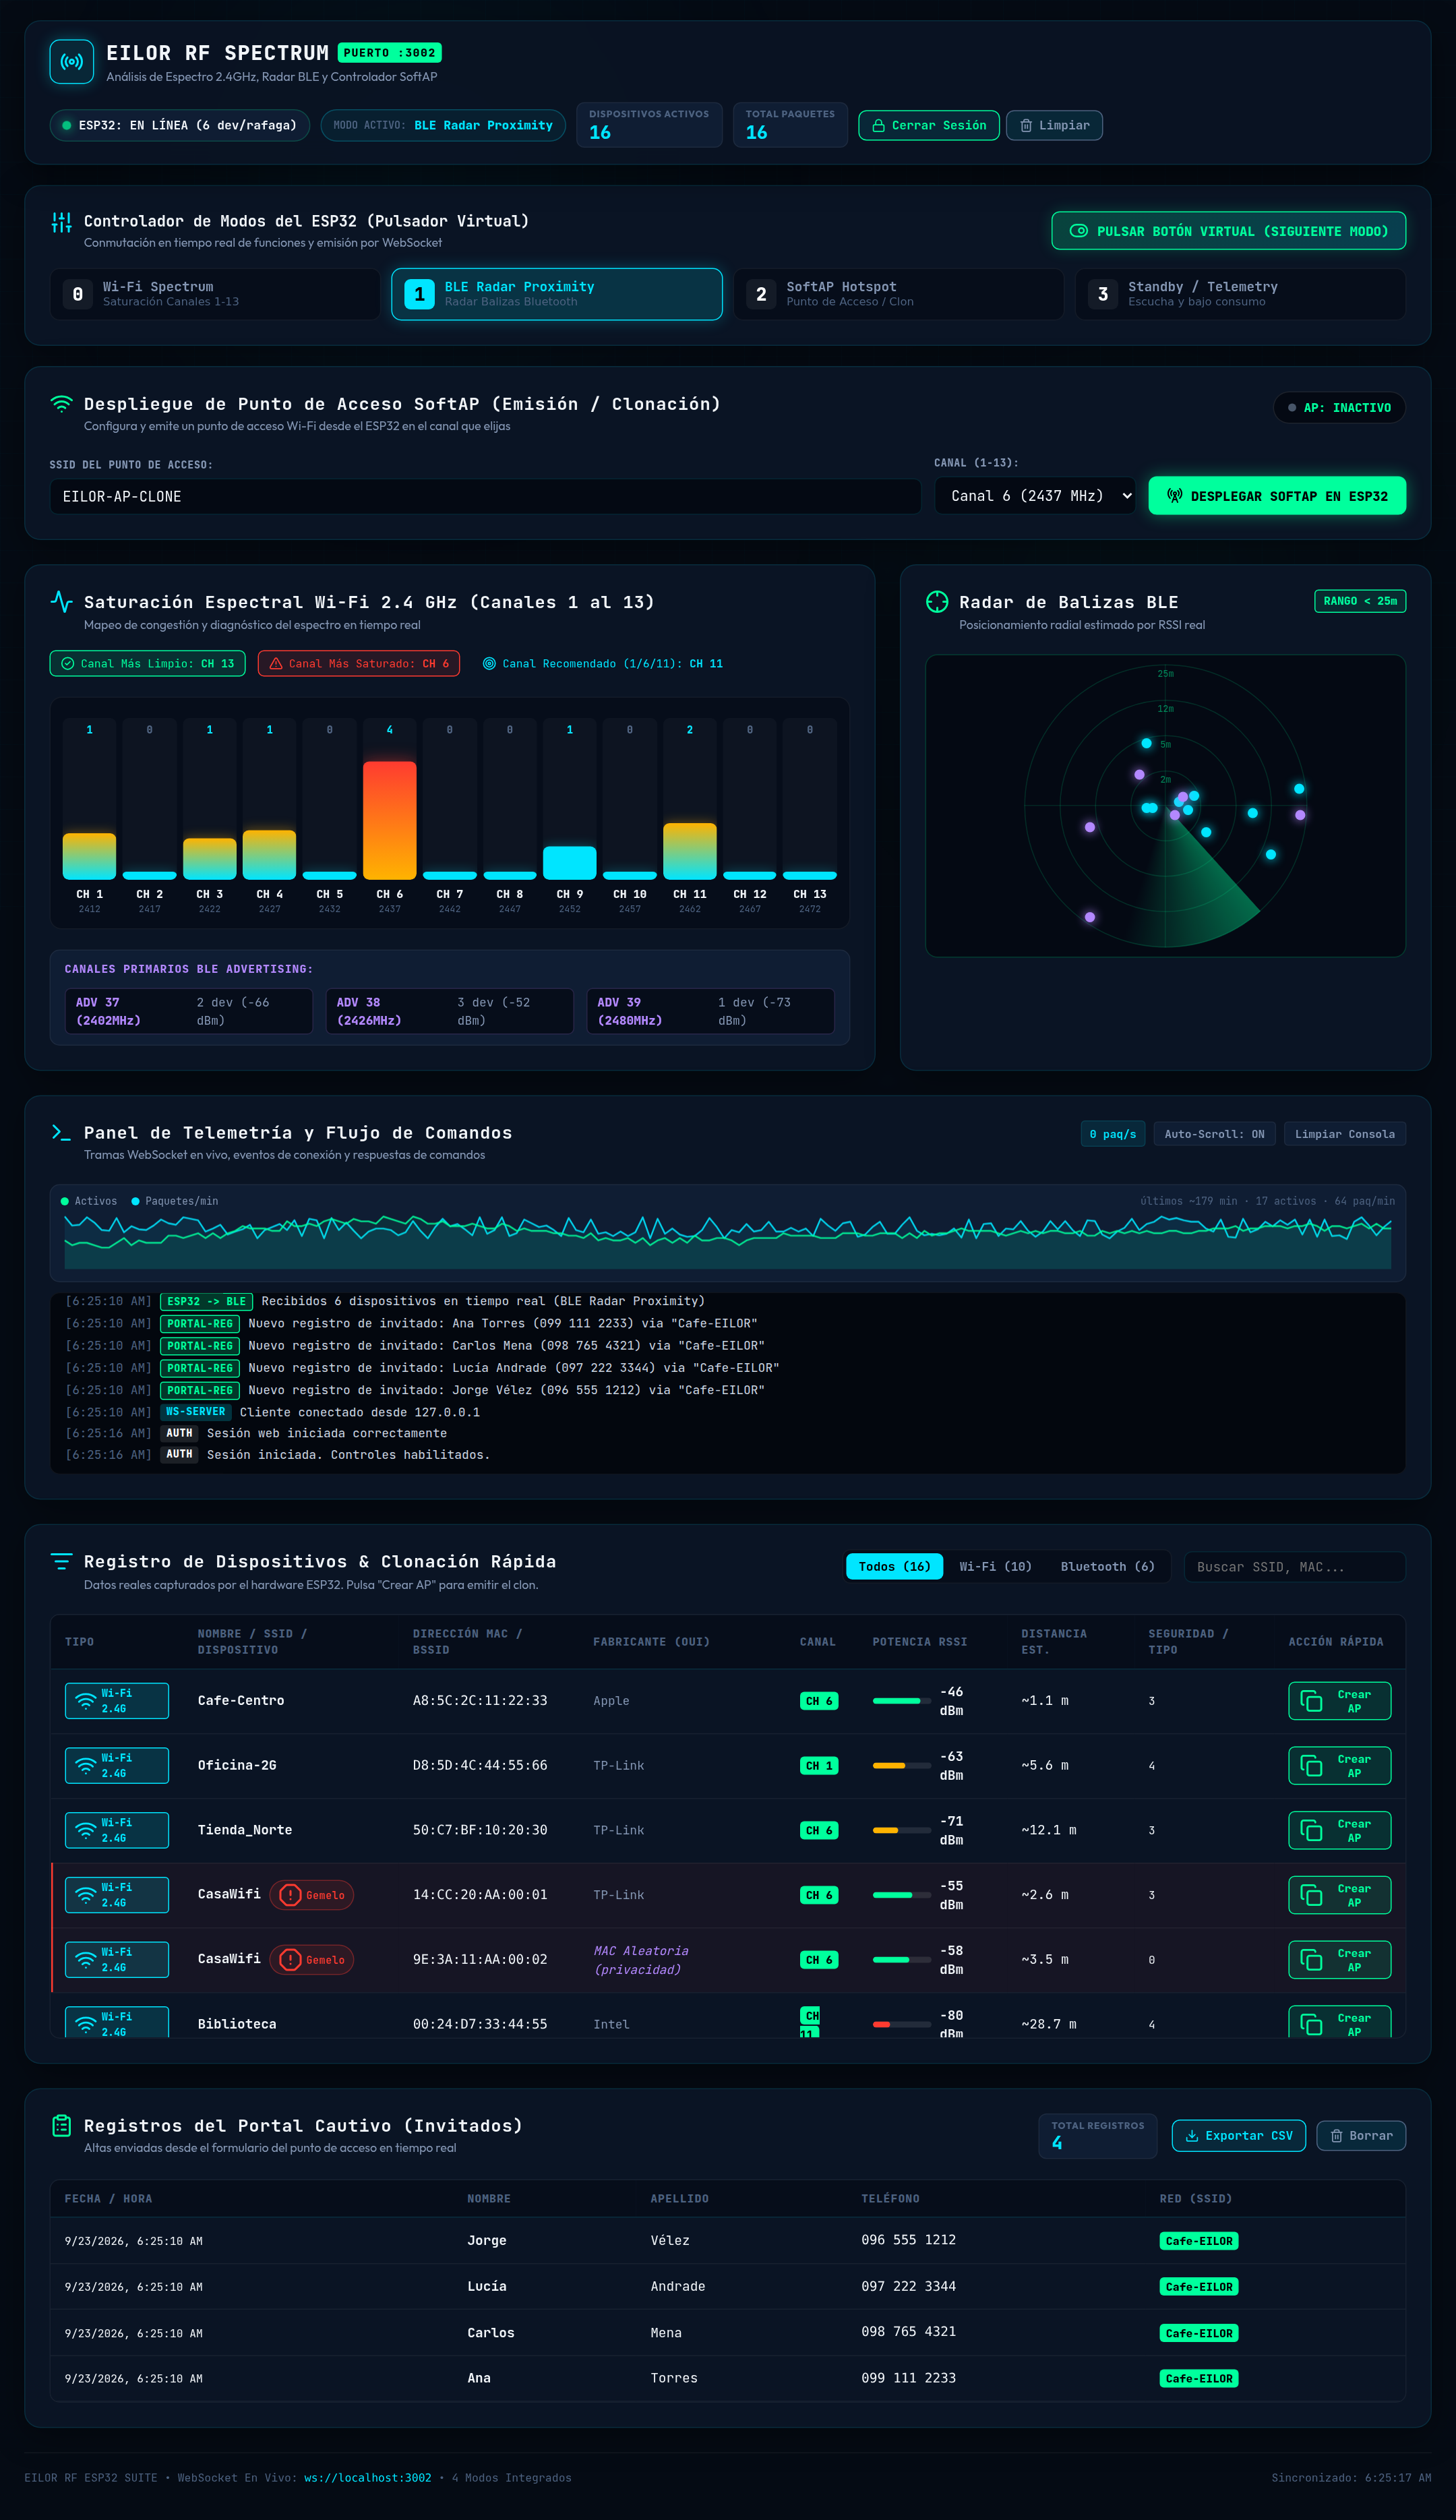
\includegraphics[width=0.98\linewidth]{figuras/cap-dashboard-full}}
\caption{Vista de referencia para validar el flujo completo después de una instalación técnica.}
\label{fig:manual-flujo}
\end{figure}
\subsection{Estructura del proyecto}
\begin{lstlisting}[style=bash,caption={Estructura de directorios},basicstyle=\ttfamily\footnotesize]
eilor/
  server.js              # servidor Express + WebSocket
  lib/                   # modulos: analysis, oui, store, auth
  public/                # dashboard: index.html, app.js, styles.css, portal-preview.html
  firmware/              # eilor_esp32.ino (firmware del ESP32)
  data/                  # persistencia JSON (se crea sola; en .gitignore)
  package.json
\end{lstlisting}

\subsection{Instalación y ejecución del servidor}
\begin{lstlisting}[style=bash,caption={Puesta en marcha del servidor},basicstyle=\ttfamily\footnotesize]
cd eilor
npm install                       # instala express, ws, cors
EILOR_PASSWORD="tu_clave" node server.js
# o gestionado con PM2:
pm2 start server.js --name eilor && pm2 save
\end{lstlisting}

\subsection{Variables de entorno}
\begin{table}[H]
\centering
\caption{Variables de entorno del servidor}
\label{tab:env}
\footnotesize
\begin{tabularx}{\linewidth}{@{}l X l@{}}
\toprule
\textbf{Variable} & \textbf{Función} & \textbf{Valor por defecto} \\
\midrule
\code{PORT} & Puerto de escucha & 3002 \\
\code{HOST} & Interfaz de escucha & 127.0.0.1 \\
\code{EILOR\_PASSWORD} & Contraseña del dashboard & Obligatoria; sin valor por defecto \\
\code{EILOR\_DEVICE\_TOKEN} & Token para restringir la ingesta & (sin definir: ingesta abierta) \\
\bottomrule
\end{tabularx}
\end{table}

\subsection{Carga del firmware}
El firmware se compila y sube desde Arduino IDE o PlatformIO. Debe ubicarse en una carpeta con su mismo nombre. Antes de compilar se configuran las credenciales Wi\nobreakdash-Fi, el \code{WS\_SERVER\_HOST} y, opcionalmente, el \code{DEVICE\_TOKEN} y el nombre del portal (\code{PORTAL\_TITULO}). Librerías requeridas: \code{WebSockets} (Markus Sattler), \code{Adafruit\_SSD1306}, \code{Adafruit\_GFX} y \code{ezButton}.

Después de cargar el firmware, abrir el monitor serie a 115200~baudios y comprobar,
en orden, la inicialización de la OLED, la asociación Wi\nobreakdash-Fi, la conexión
TLS y los mensajes de cambio de modo. Si la pantalla no inicia, comprobar VCC,
GND, SDA, SCL y la dirección I\textsuperscript{2}C antes de volver a grabar. Para
actualizar varias unidades se debe conservar el mismo identificador lógico del
dispositivo únicamente cuando cada unidad tenga su propio token y registro de
inventario.

\subsection{Prueba técnica de aceptación}
La siguiente lista permite cerrar una instalación con evidencia reproducible:
\begin{enumerate}[leftmargin=1.8em]
  \item El servidor inicia sin errores y responde en el puerto configurado.
  \item El dashboard permite iniciar sesión y cambia a solo lectura cuando se cierra sesión.
  \item El ESP32 aparece en línea y envía al menos un heartbeat.
  \item El modo Wi\nobreakdash-Fi actualiza redes y el radar BLE actualiza dispositivos.
  \item El botón cambia entre los cuatro modos sin rebotes visibles.
  \item El SoftAP entrega una IP, muestra clientes en la OLED y presenta el portal.
  \item Un registro sin conexión queda en cola y se reenvía al recuperar el WebSocket.
  \item La exportación CSV y la limpieza solo funcionan con sesión autenticada.
\end{enumerate}

La evidencia mínima debe incluir una captura de la cabecera, una del modo de
escaneo, una del portal y una del registro recibido. Estas imágenes se conservan
junto con la fecha, versión del firmware y configuración del servidor.

\subsection{Publicación con Cloudflare Tunnel}
\begin{lstlisting}[style=bash,caption={Publicación del servicio con cloudflared},basicstyle=\ttfamily\footnotesize]
cloudflared tunnel create eilor-tunnel
cloudflared tunnel route dns eilor-tunnel esp.tu-dominio.com
cloudflared tunnel run eilor-tunnel   # usa el config.yml del Cap. 8
\end{lstlisting}

\subsection{Resolución de problemas frecuentes}
\begin{itemize}[leftmargin=1.4em]
  \item \textbf{OLED apagada o con basura:} comprobar 3V3/GND, invertir SDA/SCL solo si el módulo lo exige y verificar la dirección 0x3C.
  \item \textbf{ESP32 reinicia al escanear:} sustituir el cable o fuente por una capaz de entregar al menos 500~mA y comprobar que no se estén usando dos fuentes.
  \item \textbf{ESP32 marca "sin conexión":} verificar credenciales Wi\nobreakdash-Fi, hora del sistema, alcance del túnel y que el servidor esté en línea (\code{pm2 logs eilor}).
  \item \textbf{El botón cambia dos modos:} revisar el cable entre GPIO15 y GND y mantener el antirrebote de 50~ms del firmware.
  \item \textbf{El portal no aparece:} confirmar que el dispositivo está en modo 2 y abrir \code{http://192.168.4.1}.
  \item \textbf{Registros no llegan:} revisar el enlace WebSocket y el contador de clientes; el \emph{buffer} reenviará al reconectar mientras no se alcance su capacidad.
  \item \textbf{Ingesta rechazada (401):} el servidor tiene \code{EILOR\_DEVICE\_TOKEN} definido; configurar el mismo token en el firmware.
  \item \textbf{Dashboard sin datos:} recargar el navegador, confirmar la sesión y revisar que el puerto del servidor coincida con el configurado en el túnel.
\end{itemize}

\subsection{Mantenimiento, respaldo y seguridad}
Antes de modificar firmware o servidor se debe copiar la carpeta \code{data/}, el
archivo de configuración del túnel y la versión actualmente operativa. Las
credenciales Wi\nobreakdash-Fi, la contraseña del dashboard y el token del dispositivo
no deben publicarse en el repositorio. Se recomienda rotarlos cuando cambie el
operador, limitar el acceso al dashboard mediante HTTPS y revisar periódicamente
los registros almacenados. La carcasa debe abrirse con la alimentación desconectada
y las pilas deben retirarse antes de intervenir el cableado.


% ---- ENTREGA 4: CIERRE Y SUSTENTACIÓN ----
%============================ CONCLUSIONES (ENTREGA 4) ======================
\chapter{Conclusiones y recomendaciones}
\label{cap:conclusiones}

Este capítulo presenta el cierre general del proyecto EILOR. Las conclusiones
integran los resultados funcionales, técnicos y formativos, y explicitan las
limitaciones que deben considerarse al interpretar el prototipo. Finalmente se
formulan recomendaciones concretas para su uso responsable y evolución.

\section{Conclusiones generales y limitaciones}

\begin{enumerate}[leftmargin=1.8em]
  \item \textbf{La solución cumple el objetivo general planteado.} EILOR integra
  un ESP32, un servidor Node.js y un dashboard web para observar la banda de
  2.4~GHz, identificar dispositivos y administrar una red propia de invitados.
  Las pruebas funcionales confirmaron el escaneo Wi\nobreakdash-Fi, el radar BLE,
  el SoftAP, el portal cautivo y la actualización en tiempo real. La conclusión
  se limita a las tecnologías y condiciones evaluadas; el prototipo no pretende
  sustituir un analizador de espectro profesional ni una auditoría especializada.

  \item \textbf{La arquitectura de tres capas es viable, reproducible y de bajo
  costo.} La comunicación mediante WebSocket, persistencia local y publicación
  mediante túnel TLS permitió obtener una mediana de 2.5~ms entre la ingesta y la
  difusión de eventos, con un costo estimado de hardware de USD~24.20 por unidad.
  La persistencia en archivos JSON resulta adecuada para una demostración y una
  instalación pequeña, pero limita las consultas, la concurrencia y la retención
  cuando aumenta el volumen de datos.

  \item \textbf{Los indicadores de radio son útiles para diagnóstico relativo.}
  El puntaje de interferencia, la recomendación de canales, el RSSI, el catálogo
  OUI y la detección de SSID repetidos aportan información operativa para localizar
  congestión y cambios en el entorno. Sin embargo, el RSSI no proporciona una
  distancia métrica precisa y la heurística de gemelo malicioso puede producir
  falsos positivos en redes mesh o falsos negativos ante una clonación más avanzada.

  \item \textbf{La seguridad implementada protege el flujo básico, pero no alcanza
  un perfil de producción endurecido.} La validación de sesión y token de
  dispositivo, las respuestas 401/200 y el transporte TLS/WSS reducen el acceso no
  autorizado en el escenario probado. Persisten limitaciones: la contraseña del
  dashboard requiere un mecanismo de hashing y control de intentos, los tokens
  deben rotarse y el despliegue depende de la protección de las credenciales y de
  la configuración del túnel.

  \item \textbf{El principal valor de EILOR es formativo y de gestión responsable.}
  El proyecto hace observables conceptos como interferencia, BLE, OUI,
  aleatorización de MAC, portal cautivo y autenticación, con hardware accesible y
  código auditable. Su uso válido se restringe a redes propias, información de
  baliza públicamente radiada y registros obtenidos con aviso y consentimiento;
  no cubre 5~GHz/6~GHz, no decodifica tráfico de terceros y no autoriza la
  suplantación de redes ajenas.
\end{enumerate}

\section{Recomendaciones}

\begin{enumerate}[leftmargin=1.8em]
  \item \textbf{Endurecer la autenticación antes de cualquier despliegue real:}
  almacenar contraseñas con hashing y sal, limitar intentos de inicio de sesión,
  rotar periódicamente el token del dispositivo y mantener un registro de auditoría.

  \item \textbf{Migrar la persistencia cuando crezca el volumen:} sustituir los
  archivos JSON por SQLite en instalaciones pequeñas o PostgreSQL en la nube,
  conservando la interfaz de \code{lib/store} para no acoplar la lógica de negocio
  al motor de almacenamiento.

  \item \textbf{Calibrar y documentar cada instalación:} registrar ubicación,
  orientación de la antena, tipo de carcasa, fuente de alimentación y condiciones
  del entorno; interpretar RSSI y recomendación de canal como tendencias relativas,
  no como mediciones absolutas.

  \item \textbf{Aplicar un protocolo de privacidad y operación:} usar únicamente
  SSID propios e identificables, mostrar el aviso del portal, solicitar los datos
  mínimos, restringir las exportaciones CSV, definir un periodo de retención y
  retirar las credenciales del código fuente antes de publicar el firmware.

  \item \textbf{Ampliar la validación de forma gradual:} probar el sistema durante
  periodos prolongados y con varios dispositivos, comparar resultados en distintos
  entornos y, solo después, evaluar soporte multi-dispositivo, analítica histórica,
  cobertura de 5~GHz y escalamiento del WebSocket mediante un broker.
\end{enumerate}

\noindent En conjunto, EILOR queda validado como prototipo funcional, económico y
didáctico para monitoreo responsable de redes propias. Las recomendaciones definen
las condiciones mínimas para pasar de una demostración controlada a una operación
más robusta, segura y mantenible.


%============================ REFERENCIAS ===================================
\cleardoublepage
\phantomsection\addcontentsline{toc}{chapter}{Referencias bibliográficas}
\printbibliography[title={Referencias bibliográficas}]

%============================ ANEXOS ========================================
%============================ ANEXOS ========================================
\appendix
\chapter{Glosario de términos}
\label{anexo:glosario}
\begin{description}[leftmargin=2.2cm,style=nextline]
  \item[BLE] Bluetooth Low Energy; variante de bajo consumo del estándar Bluetooth.
  \item[BSSID] Identificador único (dirección MAC) de un punto de acceso Wi\nobreakdash-Fi.
  \item[Evil twin] Punto de acceso que suplanta el SSID de una red legítima.
  \item[Heatmap] Mapa de calor; representación de la ocupación por canal.
  \item[OUI] Organizationally Unique Identifier; prefijo de fabricante en la MAC.
  \item[Portal cautivo] Página que intercepta la navegación de un cliente recién conectado.
  \item[RSSI] Received Signal Strength Indicator; indicador de intensidad de señal.
  \item[SoftAP] Punto de acceso Wi\nobreakdash-Fi emitido por software desde el propio dispositivo.
  \item[SSID] Nombre público de una red Wi\nobreakdash-Fi.
  \item[WebSocket] Protocolo de comunicación bidireccional persistente sobre TCP.
  \item[WSS] WebSocket sobre TLS (cifrado).
\end{description}

\chapter{Referencias del código fuente}
\label{anexo:codigo}
El código fuente completo del sistema acompaña a este documento. La Tabla~\ref{tab:fuentes} enumera los archivos principales y su extensión.

\begin{table}[H]
\centering
\caption{Archivos de código fuente del proyecto}
\label{tab:fuentes}
\footnotesize
\begin{tabularx}{\linewidth}{@{}l r X@{}}
\toprule
\textbf{Archivo} & \textbf{Líneas} & \textbf{Descripción} \\
\midrule
\code{firmware/eilor\_esp32.ino} & 777 & Firmware del ESP32 (4 modos, portal cautivo, buffer) \\
\code{server.js} & 665 & Servidor Express + WebSocket + API REST \\
\code{lib/analysis.js} & 71 & Puntaje de canal y detección de gemelo malicioso \\
\code{lib/oui.js} & 62 & Fabricante por OUI y MAC aleatorias \\
\code{lib/store.js} & 81 & Persistencia JSON y series temporales \\
\code{lib/auth.js} & 60 & Sesiones por token y autorización \\
\code{public/app.js} & 913 & Lógica del dashboard en tiempo real \\
\code{public/index.html} & 419 & Estructura del dashboard \\
\code{public/styles.css} & 1272 & Estilos del tablero \\
\bottomrule
\end{tabularx}
\end{table}

\chapter{Repositorio y despliegue de referencia}
\label{anexo:repositorio}

El código fuente completo del proyecto (firmware, servidor, módulos y frontend) se
aloja en el siguiente repositorio, que acompaña a este documento como anexo digital:

\begin{itemize}[leftmargin=1.4em]
  \item \textbf{Repositorio de código:} \repourl
  \item \textbf{Plataforma en producción:} \plataformaurl
  \item \textbf{Túnel y hostname público:} \code{esp.orellanadigitalco.trade} (puerto 443, WSS/HTTPS), publicado con Cloudflare Tunnel (Capítulo~\ref{cap:cloudflare}).
\end{itemize}

\noindent La plataforma en producción integra el flujo de extremo a extremo
descrito en el Capítulo~\ref{cap:plataforma}: el dispositivo ESP32 se conecta por
WSS al servidor a través del túnel, y los clientes web consumen el \emph{dashboard}
sobre HTTPS. Para reproducir el despliegue basta clonar el repositorio, instalar las
dependencias (\code{npm install}), definir \code{EILOR\_PASSWORD} y ejecutar el
servidor bajo PM2, siguiendo el manual técnico del Capítulo~\ref{cap:manuales}.


\end{document}
